%
% MIT License
%
% Copyright (c) 2024 Fabricio Batista Narcizo.
%
% Permission is hereby granted, free of charge, to any person obtaining a copy
% of this software and associated documentation files (the "Software"), to deal
% in the Software without restriction, including without limitation the rights
% to use, copy, modify, merge, publish, distribute, sublicense, and/or sell
% copies of the Software, and to permit persons to whom the Software is
% furnished to do so, subject to the following conditions:
%
% The above copyright notice and this permission notice shall be included in
% all copies or substantial portions of the Software.
%
% THE SOFTWARE IS PROVIDED "AS IS", WITHOUT WARRANTY OF ANY KIND, EXPRESS OR
% IMPLIED, INCLUDING BUT NOT LIMITED TO THE WARRANTIES OF MERCHANTABILITY,
% FITNESS FOR A PARTICULAR PURPOSE AND NONINFRINGEMENT. IN NO EVENT SHALL THE
% AUTHORS OR COPYRIGHT HOLDERS BE LIABLE FOR ANY CLAIM, DAMAGES OR OTHER
% LIABILITY, WHETHER IN AN ACTION OF CONTRACT, TORT OR OTHERWISE, ARISING FROM,
% OUT OF OR IN CONNECTION WITH THE SOFTWARE OR THE USE OR OTHER DEALINGS IN THE
% SOFTWARE.
%

% The ITU template is based on the ABNTex2 class, which is a LaTeX class for
% writing documents following the Brazilian Association of Technical Standards
% (ABNT) standards. This document uses arabic number and the first paragraphs
% of each chapter doesn't have spacing.
\documentclass[pnumromarab,noindentfirst]{abnt}


% -----------------------------------------------------------------------------
% ITU Package and Related Dependencies
% -----------------------------------------------------------------------------
\usepackage{ITU}  % ITU package for formatting (specific to ITU use)
\pagestyle{itu}   % Define the header and footer style for ITU format


% -----------------------------------------------------------------------------
% General Utility Packages
% -----------------------------------------------------------------------------

% Encoding and fonts.
\usepackage{type1cm}  % Custom section heading font size.

% Document formatting and structure.
\usepackage{pdflscape}  % Landscape orientation for some pages.
\usepackage{pdfpages}   % Embed external PDF files.
\usepackage{comment}    % Block comment support.

% Text and color formatting.
\usepackage{xcolor}           % Text color customization.
\usepackage{lettrine}         % Drop caps (decorative first letter).
\usepackage{hologo}           % Typeset TeX-related logos.
\usepackage{color, colortbl}  % Table cell coloring

% Graphics and figures.
\usepackage{graphicx}                    % To include images.
\graphicspath{{./images/}}               % Path for image files.
\usepackage{float}                       % Control figure/table placement.
\usepackage{subcaption}                  % Support for subfigures.
\usepackage[font=footnotesize]{caption}  % Customize figure/table captions.
\usepackage{tikz} 					     % Drawing package.
\usepackage{pgfplots} 					 % Plotting package.
\usepackage{readarray} 				     % Read arrays from external files.

% Lists.
\usepackage{paralist}             % Inline or compact list environments.
\usepackage{enumerate}            % Extended enumerate lists.
\usepackage[ampersand]{easylist}  % Easy-to-use custom lists.

% Tables.
\usepackage{longtable}       % Multi-page tables
\usepackage{multirow}        % Cells spanning multiple rows
\usepackage{bigstrut}        % Adjust vertical spacing in table rows
\usepackage{array}           % Enhanced table column formatting
\usepackage{calc}            % Arithmetic for table dimensions
\usepackage{setspace}        % Custom text spacing
\usepackage{booktabs}        % Professional-quality tables.
\usepackage{threeparttable}  % Three-part tables.

% Math and symbols.
\usepackage{amsmath, amssymb}  % Advanced mathematical typesetting.
\usepackage{mathtools}         % Advanced math tools.

% Links and URLs.
\usepackage[colorlinks=false]{hyperref}  % For hyperlinks (color disabled).
\usepackage{bookmark}                    % Enhanced bookmark control.

% Citations and references.
\usepackage[nocompress]{cite}  % To manage citation ordering.

% Code and listings.
\usepackage{listings}  % To print source code in the document.

% Glossaries and acronyms.
\usepackage[acronym,nonumberlist]{glossaries}  % Acronym and glossary support.


% -----------------------------------------------------------------------------
% Color Definitions
% -----------------------------------------------------------------------------
\definecolor{Gray}{gray}{0.8} 
\definecolor{halfgray}{gray}{0.55}
\definecolor{ipython_frame}{RGB}{207, 207, 207}
\definecolor{ipython_bg}{RGB}{247, 247, 247}
\definecolor{ipython_red}{RGB}{186, 33, 33}
\definecolor{ipython_green}{RGB}{0, 128, 0}
\definecolor{ipython_cyan}{RGB}{64, 128, 128}
\definecolor{ipython_purple}{RGB}{170, 34, 255}


% -----------------------------------------------------------------------------
% Mathematical Tools
% -----------------------------------------------------------------------------
\DeclarePairedDelimiter\abs{\lvert}{\rvert}   % Absolute value
\DeclarePairedDelimiter\norm{\lVert}{\rVert}  % Norm


% -----------------------------------------------------------------------------
% Table Formatting Packages
% -----------------------------------------------------------------------------

% Custom Column Types.
\newcolumntype{L}[1]{>{\raggedright\let\newline\\\arraybackslash\hspace{0pt}}p{#1}}  % Left-aligned.
\newcolumntype{C}[1]{>{\centering\let\newline\\\arraybackslash\hspace{0pt}}p{#1}}  % Centered.
\newcolumntype{R}[1]{>{\raggedleft\let\newline\\\arraybackslash\hspace{0pt}}p{#1}}  % Right-aligned.


% -----------------------------------------------------------------------------
% TikZ and PGFPlots Configuration
% -----------------------------------------------------------------------------
\usepgfplotslibrary{groupplots}
\usetikzlibrary{calc,intersections,quotes,angles,external,patterns,positioning}
\usetikzlibrary{external}
\tikzexternalize[prefix=tikz/]
\pgfplotsset{compat=1.18}
\providecommand\mathdefault[1]{#1}


% -----------------------------------------------------------------------------
% Python Language Formatting
% -----------------------------------------------------------------------------
\lstdefinelanguage{Python}{
	morekeywords={access,and,break,class,continue,def,del,elif,else,except,exec,finally,for,from,global,if,import,in,is,lambda,not,or,pass,print,raise,return,try,while},
	morekeywords=[2]{abs,all,any,basestring,bin,bool,bytearray,callable,chr,classmethod,cmp,compile,complex,delattr,dict,dir,divmod,enumerate,eval,execfile,file,filter,float,format,frozenset,getattr,globals,hasattr,hash,help,hex,id,input,int,isinstance,issubclass,iter,len,list,locals,long,map,max,memoryview,min,next,object,oct,open,ord,pow,property,range,raw_input,reduce,reload,repr,reversed,round,set,setattr,slice,sorted,staticmethod,str,sum,super,tuple,type,unichr,unicode,vars,xrange,zip,apply,buffer,coerce,intern},
	sensitive=true,
	morecomment=[l]\#,
	morestring=[b]',
	morestring=[b]",
	morestring=[s]{'''}{'''},
	morestring=[s]{"""}{"""},
	morestring=[s]{r'}{'},
	morestring=[s]{r"}{"},
	morestring=[s]{r'''}{'''},
	morestring=[s]{r"""}{"""},
	morestring=[s]{u'}{'},
	morestring=[s]{u"}{"},
	morestring=[s]{u'''}{'''},
	morestring=[s]{u"""}{"""},
	% {replace}{replacement}{lenght of replace}
	% *{-}{-}{1} will not replace in comments and so on
	literate=
	{á}{{\'a}}1 {é}{{\'e}}1 {í}{{\'i}}1 {ó}{{\'o}}1 {ú}{{\'u}}1
	{Á}{{\'A}}1 {É}{{\'E}}1 {Í}{{\'I}}1 {Ó}{{\'O}}1 {Ú}{{\'U}}1
	{à}{{\`a}}1 {è}{{\`e}}1 {ì}{{\`i}}1 {ò}{{\`o}}1 {ù}{{\`u}}1
	{À}{{\`A}}1 {È}{{\'E}}1 {Ì}{{\`I}}1 {Ò}{{\`O}}1 {Ù}{{\`U}}1
	{ä}{{\"a}}1 {ë}{{\"e}}1 {ï}{{\"i}}1 {ö}{{\"o}}1 {ü}{{\"u}}1
	{Ä}{{\"A}}1 {Ë}{{\"E}}1 {Ï}{{\"I}}1 {Ö}{{\"O}}1 {Ü}{{\"U}}1
	{â}{{\^a}}1 {ê}{{\^e}}1 {î}{{\^i}}1 {ô}{{\^o}}1 {û}{{\^u}}1
	{Â}{{\^A}}1 {Ê}{{\^E}}1 {Î}{{\^I}}1 {Ô}{{\^O}}1 {Û}{{\^U}}1
	{œ}{{\oe}}1 {Œ}{{\OE}}1 {æ}{{\ae}}1 {Æ}{{\AE}}1 {ß}{{\ss}}1
	{ç}{{\c c}}1 {Ç}{{\c C}}1 {ø}{{\o}}1 {å}{{\r a}}1 {Å}{{\r A}}1
	{€}{{\EUR}}1 {£}{{\pounds}}1
	%
	{^}{{{\color{ipython_purple}\^{}}}}1
	{=}{{{\color{ipython_purple}=}}}1
	%
	{+}{{{\color{ipython_purple}+}}}1
	{*}{{{\color{ipython_purple}$^\ast$}}}1
	{/}{{{\color{ipython_purple}/}}}1
	%
	{+=}{{{+=}}}1
	{-=}{{{-=}}}1
	{*=}{{{$^\ast$=}}}1
	{/=}{{{/=}}}1,
	literate=
	*{-}{{{\color{ipython_purple}-}}}1
		{?}{{{\color{ipython_purple}?}}}1,
	%
	identifierstyle=\color{black}\ttfamily,
	commentstyle=\color{ipython_cyan}\ttfamily,
	stringstyle=\color{ipython_red}\ttfamily,
	keepspaces=true,
	showspaces=false,
	showstringspaces=false,
	rulecolor=\color{ipython_frame},
	frame=single,
	frameround={t}{t}{t}{t},
	framexleftmargin=6mm,
	numbers=left,
	numberstyle=\tiny\color{halfgray},
	backgroundcolor=\color{ipython_bg},
	% extendedchars=true,
	basicstyle=\scriptsize,
	keywordstyle=\color{ipython_green}\ttfamily,
}


% -----------------------------------------------------------------------------
% Glossary compilation
% -----------------------------------------------------------------------------

% IMPORTANT: You must execute the following command in the terminal to compile
% the glossary: `makeglossaries thesis`
\makeglossaries
\newacronym{abnt}{ABNT}{Brazilian Association of Technical Standards}
\newacronym{abnt-dk}{ABNT}{Den Brasilianske Standardiseringsorganisation}
\newacronym{itu}{ITU}{IT University of Copenhagen}


% -----------------------------------------------------------------------------
% Main Document
% -----------------------------------------------------------------------------
\begin{document}


% -----------------------------------------------------------------------------
% Basic Information
% -----------------------------------------------------------------------------
\university{IT University of Copenhagen}       % University name
\departament{Computer Science Department}      % Department name
\program{Ph.D. Programme in Computer Science}  % Bachelor's Programme in Software Development, Master's Programme in Software Design, or Ph.D. Programme in Computer Science
\maintitle{Title of the Thesis}      % Main title
\subtitle{Ph.D. Thesis}              % Bachelor's Thesis, or Master's Thesis
\author{Student's Name}              % Author's name
\supervisor{Supervisor's Name}     	 % Supervisor's name
\cosupervisor{Co-Supervisor's Name}  % Co-Supervisor's name
\city{Copenhagen -- Denmark}         % City and country
\info{November, 2024}                % Month and year

% Previous academic degrees
\previousDegrees{B.Sc. University of the West of Santa Catarina, 2005}
				{M.Sc. Technological Institute of Aeronautics, 2008}

% Examination committee members
\committeeMemberA{Committee Member A}
\committeeMemberB{Committee Member B}
\committeeMemberC{Committee Member C}


% -----------------------------------------------------------------------------
% Dedication
% -----------------------------------------------------------------------------
\dedication{This Ph.D. thesis is dedicated to all the \LaTeX~errors that tested my patience, the compiler warnings that kept me humble, and the endless debug sessions that taught me resilience. Without them, this journey would have been far too easy-and far less memorable.

And to coffee, for being the true unsung hero of this endeavor.}


% -----------------------------------------------------------------------------
% Epigraph
% -----------------------------------------------------------------------------
\epigraph{``With regard to performance, commitment, effort,\\
	dedication, there is no middle ground.\\
	Or you do something very well or not at all.''\\}{\\
	Ayrton Senna do Brasil (1960-1994)}


% -----------------------------------------------------------------------------
% Cover and Preliminaries
% -----------------------------------------------------------------------------

% Generate the cover page
\cover

% Additional preliminary pages
\coversheet  % Cover sheet

\approvalsheet  % Approval sheet

\dedicationpage  % Dedication page

% Acknowledgment section
\acknowledgment{Gratitude is one of the noblest feelings of a man. Thus, I could not fail to mention that the accomplishment of this work is the result of the collaboration of many people. I would like to express my gratitude in a particular way.

I would like to thank the one person without whom this document would never have seen the light of day: me. Yes, that's right--me. For not only creating this \LaTeX~template, but also generously sharing it with the students of this esteemed university. Truly, my brilliance knows no bounds, and my magnanimity knows no limits.

I must also thank my coffee mug, which stood loyally by my side through countless lines of code, offering solace and caffeination in equal measure. Finally, a nod to my keyboard, whose steadfast resilience endured my furious typing as I resolved bugs and made this template a reality.

To the students who will use this template: you're welcome.}
\acknowledgmentpage  % Acknowledgment page

% Epigraph page
\epigraphpage


% -----------------------------------------------------------------------------
% Abstract
% -----------------------------------------------------------------------------
\begin{abstract}
This document introduces a custom \LaTeX~template designed to simplify students' lives at IT University of Copenhagen, empowering them to create beautifully formatted academic documents with minimal effort. The template encapsulates the \acrfull{abnt} formatting guidelines while incorporating features that enhance usability, adaptability, and visual appeal. By providing this template, we aim to reduce formatting-related stress, encourage consistent document presentation, and gently guide students into the wonderful (and occasionally maddening) world of \LaTeX. Whether you are writing a thesis, report, or any academic work, this template is your steadfast companion. Just don't forget to thank the creator in your acknowledgments.\\
\textbf{Keywords:} \LaTeX, template, thesis, computer science, IT University of Copenhagen.
\end{abstract}

% Resume section (in Danish)
\begin{resume}
Dette dokument introducerer en skr{\ae}ddersyet \LaTeX-skabelon, der er designet til at g{\o}re livet lettere for studerende p{\aa} IT-Universitetet i K{\o}benhavn. Skabelonen g{\o}r det muligt for dem at skabe smukt formaterede akademiske dokumenter med minimal indsats. Skabelonen overholder retningslinjerne fra \acrfull{abnt-dk} og indeholder samtidig funktioner, der forbedrer brugervenlighed, tilpasning og {\ae}stetik. Med denne skabelon str{\ae}ber vi efter at reducere stress forbundet med formatering, fremme ensartet pr{\ae}sentation af dokumenter og blidt introducere de studerende til den fantastiske (og til tider frustrerende) verden af \LaTeX. Uanset om du skriver en afhandling, en rapport eller et andet akademisk arbejde, er denne skabelon din trofaste f{\o}lgesvend. Husk blot at takke skaberen i dine taksigelser.\\
\textbf{N{\o}gleord:} \LaTeX, skabelon, afhandling, datalogi, IT-Universitetet i K{\o}benhavn.
\end{resume}


% -----------------------------------------------------------------------------
% Pre-Textual Elements
% -----------------------------------------------------------------------------
\listoffigures                                            % List of Figures
\listoftables                                             % List of Tables
\printglossary[title=List of Acronyms,type=\acronymtype]  % List of Acronyms
\contents                                                 % Table of contents


% -----------------------------------------------------------------------------
% Chapters
% -----------------------------------------------------------------------------

% Part I: Foundations and Context.
\part{Foundations and Context}\label{par:introduction}
%
% MIT License
%
% Copyright (c) 2024 Fabricio Batista Narcizo.
%
% Permission is hereby granted, free of charge, to any person obtaining a copy
% of this software and associated documentation files (the "Software"), to deal
% in the Software without restriction, including without limitation the rights
% to use, copy, modify, merge, publish, distribute, sublicense, and/or sell
% copies of the Software, and to permit persons to whom the Software is
% furnished to do so, subject to the following conditions:
%
% The above copyright notice and this permission notice shall be included in
% all copies or substantial portions of the Software.
%
% THE SOFTWARE IS PROVIDED "AS IS", WITHOUT WARRANTY OF ANY KIND, EXPRESS OR
% IMPLIED, INCLUDING BUT NOT LIMITED TO THE WARRANTIES OF MERCHANTABILITY,
% FITNESS FOR A PARTICULAR PURPOSE AND NONINFRINGEMENT. IN NO EVENT SHALL THE
% AUTHORS OR COPYRIGHT HOLDERS BE LIABLE FOR ANY CLAIM, DAMAGES OR OTHER
% LIABILITY, WHETHER IN AN ACTION OF CONTRACT, TORT OR OTHERWISE, ARISING FROM,
% OUT OF OR IN CONNECTION WITH THE SOFTWARE OR THE USE OR OTHER DEALINGS IN THE
% SOFTWARE.
%

% Introduction Chapter.
\chapter{Introduction}\label{chap:introduction}
\lettrine[lines=3]{T}{his} \LaTeX~template provides a structured and professional foundation for the bachelor's, master's, and Ph.D. students from the \href{http://itu.dk}{\acrfull{itu}}, ensuring consistency, clarity, and ease of use as they develop their theses. The students can use this template to guide them in organizing their work effectively, allowing them to focus on the content while adhering to academic formatting standards.

The introduction chapter is where you set the stage for your thesis. It provides the reader with the necessary background, clearly defines the problem, and outlines the goals and significance of your study. This chapter serves as a roadmap for the rest of the thesis, giving the audience a clear understanding of what to expect and why your work matters.

\section{Background and Context}\label{sec:background-context}
This section introduces the reader to the broader context of your research area. You should:
\begin{enumerate}
	\item \textbf{Describe the Field:} Provide an overview of your work's domain or discipline. Discuss recent trends or developments that make your research relevant.
	\item \textbf{Highlight the Motivation:} Explain what motivated you to pursue this topic. This might include societal challenges, technological advancements, or gaps in existing knowledge.
\end{enumerate}

Keep this section concise but informative. The goal is to give the reader enough context to appreciate the importance of the problem you aim to solve.

\section{Problem Statement}\label{sec:problem-statement}
Here, you define the specific problem your research addresses. This section should include:
\begin{enumerate}
	\item \textbf{Current Challenges:} Summarize the key issues or limitations in the current state of knowledge or practice.
    \item \textbf{Focus of the Study:} Clearly articulate the specific problem you aim to solve, ensuring it is well-defined and measurable.
\end{enumerate}

A well-written problem statement helps the reader immediately grasp your thesis's core issue.

\section{Objectives of the Study}\label{sec:objectives}
In this section, clearly outline the goals of your research. These objectives should be specific, measurable, and aligned with the problem statement. Use bullet points or numbered lists to make them easy to read. For example:
\begin{itemize}
	\item \textit{To analyze\dots}
    \item \textit{To develop\dots}
    \item \textit{To evaluate\dots}
\end{itemize}

Ensure your objectives are realistic and achievable within the scope of your thesis.

\section{Research Questions and Hypotheses}\label{sec:research-questions}
Here, you present the research questions that guide your study. These questions should be directly related to your objectives and problem statement. If applicable, state your hypotheses, explaining the assumptions or predictions your study will test. For example:
\begin{itemize}
	\item \textbf{Research Question:} How does [variable] influence [outcome]?
    \item \textbf{Hypothesis:} It is hypothesized that [specific prediction].
\end{itemize}

This section demonstrates the focus and clarity of your study.

\section{Scope and Limitations}\label{sec:scope-limitations}
This section defines the boundaries of your research and acknowledges its limitations. Include:
\begin{enumerate}
	\item \textbf{Scope:} Explain what your study covers (e.g., data, methods, population).
	\item \textbf{Limitations:} Be transparent about time, resources, or data availability constraints that may affect your results.
\end{enumerate}

Being upfront about the limitations, adds credibility to your work and sets realistic expectations for the reader.

\section{Significance of the Study}\label{sec:significance}
Discuss why your research is essential and its contribution to the field. Address questions like:
\begin{itemize}
	\item How does this work fill existing gaps in knowledge?
	\item What are the practical or theoretical implications of your findings?
\end{itemize}

Convince the reader that your study has meaningful value and relevance.

\section{Structure of the Thesis}\label{sec:struture-thesis}
This final section provides a brief overview of the chapters to follow. Write 1-2 sentences summarizing the content of each chapter. For example:

This thesis has six chapters, each addressing specific aspects of the research topic. The introduction composes Chapter~\ref{chap:introduction} and sets the scene for the presented research project.

Chapter~\ref{chap:review} provides a comprehensive overview of the relevant literature and existing research in the field. It critically evaluates previous works, identifies gaps in the knowledge, and establishes the theoretical foundation for the study.

Chapter~\ref{chap:methodology} describes the research approach and methods to achieve the study's objectives. It includes details on data collection, experimental design, implementation, and evaluation metrics. It also discusses ethical considerations and limitations of the methodology.

Chapter~\ref{chap:results} presents the research findings clearly and systematically. It includes data visualizations, tables, and detailed analyses to interpret the results in the context of the research questions.

Chapter~\ref{chap:discussion} provides a deeper interpretation of the results, comparing them with existing studies. It discusses the findings' implications, the study's strengths and limitations, and potential areas for future research.

Chapter~\ref{chap:conclusions} is the last chapter, and it summarizes the key findings, highlights the study's contributions, and provides actionable recommendations. It concludes with final reflections on the research and its broader impact.

%
% MIT License
%
% Copyright (c) 2024 Fabricio Batista Narcizo.
%
% Permission is hereby granted, free of charge, to any person obtaining a copy
% of this software and associated documentation files (the "Software"), to deal
% in the Software without restriction, including without limitation the rights
% to use, copy, modify, merge, publish, distribute, sublicense, and/or sell
% copies of the Software, and to permit persons to whom the Software is
% furnished to do so, subject to the following conditions:
%
% The above copyright notice and this permission notice shall be included in
% all copies or substantial portions of the Software.
%
% THE SOFTWARE IS PROVIDED "AS IS", WITHOUT WARRANTY OF ANY KIND, EXPRESS OR
% IMPLIED, INCLUDING BUT NOT LIMITED TO THE WARRANTIES OF MERCHANTABILITY,
% FITNESS FOR A PARTICULAR PURPOSE AND NONINFRINGEMENT. IN NO EVENT SHALL THE
% AUTHORS OR COPYRIGHT HOLDERS BE LIABLE FOR ANY CLAIM, DAMAGES OR OTHER
% LIABILITY, WHETHER IN AN ACTION OF CONTRACT, TORT OR OTHERWISE, ARISING FROM,
% OUT OF OR IN CONNECTION WITH THE SOFTWARE OR THE USE OR OTHER DEALINGS IN THE
% SOFTWARE.
%

% Literature Review Chapter.
\chapter{Literature Review}\label{chap:review}
\lettrine[lines=3]{T}{he} literature review chapter is where you demonstrate your understanding of the existing body of knowledge in your research area. This chapter establishes the foundation for your work, highlighting the theoretical underpinnings, critically analyzing relevant studies, and identifying research gaps that your study aims to address. A well-structured literature review is essential for establishing the credibility and significance of your research.

Start this chapter by briefly explaining its purpose. Provide a roadmap for the reader, outlining what this chapter covers. For example: ``\textit{This chapter presents the theoretical foundations of the research, analyzes the state-of-the-art literature, critically evaluates existing studies, and identifies the gaps that this thesis seeks to address}.''

\section{Theoretical Framework}\label{sec:theoretical-framework}
In this section, you should introduce the theoretical concepts and models that underpin your research. This is where you establish the theoretical foundation of your study and explain the key concepts that inform your research questions. Discuss the relevant theories, frameworks, and methodologies that guide your work. Use equations or definitions if necessary. For example, you might write: ``\textit{According to $X$ theory, you can express the relationship between $A$ and $B$ as:} $A = f(B)$.'' Or, ``\textit{The study draws on the theoretical framework of Narcizo~\cite{Narcizo2012}. Equation~\ref{eq:linear-regression} expresses his theory as:}''
\begin{equation}
    y = mx + c
    \label{eq:linear-regression}
\end{equation}
where $y$ represents the dependent variable, $m$ is the slope, and $c$ is the intercept.

% This is an example of a single-line comment in LaTeX.
If necessary, you can comment or hide some sentences in your document. In \LaTeX, comments are created using the percent symbol (\%). Any text following \% on the same line will not be compiled, making it an excellent way to add notes or explanations to your code. Use comments to clarify your code for yourself and others, but avoid overusing them to maintain readability.

% This is an example of a multi-line comment in LaTeX.
\begin{comment}
    This is a multi-line comment in LaTeX. You can use this to comment out large blocks of text or code that you don't want to compile. Multi-line comments are useful for temporarily disabling sections of your document or adding detailed explanations that you don't want to appear in the final output. Use comments to explain the purpose of a section of code, provide context for complex equations, or outline your thought process as you write.

    Remember to always thank the creator of this amazing template: Fabricio Batista Narcizo. For example:

    \textit{I would like to express my gratitude to Fabricio Batista Narcizo for creating this \LaTeX~template. It has been incredibly helpful in formatting my thesis and making my life easier with this template!}
\end{comment}

\section{State-of-the-Art Review}\label{sec:state-of-the-art}
Provide an overview of existing research in your topic area. Summarize key studies, methodologies, and findings to give the reader a comprehensive understanding of the current state of knowledge. Identify the major trends, debates, and controversies in the literature. You can organize this section thematically, chronologically, or methodologically, depending on what makes the most sense for your research.

\subsection{Overview of Existing Research in the Topic Area}\label{subsec:overview}
Briefly outline significant studies and highlight patterns or trends, for example: ``\textit{Research on this topic has grown significantly in recent years. Studies such as Narcizo~\cite{Narcizo2013} and Narcizo \etal~\cite{Narcizo2013a} provide a comprehensive analysis of eye-tracking studies.}''

\section{Critical Analysis of Related Work}\label{sec:critical-analysis}
This section is not just a summary but a critique. Compare methodologies, highlight strengths and weaknesses, and discuss how these studies inform your research. Identify gaps, contradictions, or limitations in the existing literature. For example:

The following critical points were identified in the literature:
\begin{itemize}
    \item \textbf{Strengths:} Study $A$~\cite{Narcizo2015} effectively applies method $X$ to context $Y$, demonstrating high reliability.
    \item \textbf{Weaknesses:} Study $B$~\cite{Munzlinger2012} lacks generalizability due to a small sample size.
\end{itemize}

\section{Research Gap Identification}\label{sec:research-gap}
Clearly articulate the gaps in the literature that your study addresses. This is a critical transition point that justifies your research. Explain how your work builds on existing knowledge and contributes to the field. For example: 

Despite extensive research in $XYZ$, significant gaps remain:
\begin{enumerate}
    \item Limited exploration of $ABC$ in context $DEF$.
    \item Inadequate integration of $GHI$ with $JKL$.
\end{enumerate}

This thesis aims to address these gaps by focusing on\dots

\section{Summary}\label{sec:review-summary}
Conclude the chapter with a summary that recaps the major findings from the literature and emphasizes the research gaps. For example: ``\textit{This chapter reviewed the theoretical foundations, state-of-the-art research, and critical analyses relevant to the study. Key gaps identified in the literature include \dots These findings establish the need for the research presented in the following chapters.}''


% Part II: Research Methodology and Execution.
\part{Research Methodology and Execution}\label{par:methodology}
%
% MIT License
%
% Copyright (c) 2024 Fabricio Batista Narcizo.
%
% Permission is hereby granted, free of charge, to any person obtaining a copy
% of this software and associated documentation files (the "Software"), to deal
% in the Software without restriction, including without limitation the rights
% to use, copy, modify, merge, publish, distribute, sublicense, and/or sell
% copies of the Software, and to permit persons to whom the Software is
% furnished to do so, subject to the following conditions:
%
% The above copyright notice and this permission notice shall be included in
% all copies or substantial portions of the Software.
%
% THE SOFTWARE IS PROVIDED "AS IS", WITHOUT WARRANTY OF ANY KIND, EXPRESS OR
% IMPLIED, INCLUDING BUT NOT LIMITED TO THE WARRANTIES OF MERCHANTABILITY,
% FITNESS FOR A PARTICULAR PURPOSE AND NONINFRINGEMENT. IN NO EVENT SHALL THE
% AUTHORS OR COPYRIGHT HOLDERS BE LIABLE FOR ANY CLAIM, DAMAGES OR OTHER
% LIABILITY, WHETHER IN AN ACTION OF CONTRACT, TORT OR OTHERWISE, ARISING FROM,
% OUT OF OR IN CONNECTION WITH THE SOFTWARE OR THE USE OR OTHER DEALINGS IN THE
% SOFTWARE.
%

% Methodology Chapter.
\chapter{Methodology}\label{chap:methodology}
\lettrine[lines=3]{T}{he} methodology chapter describes the approaches, tools, and processes you used to conduct your research. It should provide sufficient detail for the reader to understand how you gathered and analyzed data, making it possible for others to replicate your study if needed. This chapter demonstrates the rigor and validity of your research.

Start this chapter with a brief explanation of its purpose. Provide a roadmap for the reader. For example: ``\textit{This chapter outlines the research design, data collection methods, implementation details, evaluation metrics, and ethical considerations of this study. It provides a comprehensive explanation of the processes used to address the research questions presented in Section~\ref{sec:research-questions}}.''

\section{Research Design and Approach}\label{sec:research-design}
Describe the overall design of your study. Explain whether it is experimental, observational, qualitative, or quantitative, and justify why this approach is appropriate for addressing your research questions.

If necessary, you can include figures or diagrams to illustrate the research design. You might include a flowchart showing the sequence of steps in your study or a diagram of the experimental setup. You must insert figures after you cited them in the text, and their captions should be below the them. There are two alternatives to include figures in your document: 1) a single figure or 2) a figure with subfigures. The former is used when you want to include a single image, while the latter is used when you want to include multiple images in a single figure. For example, Figure~\ref{fig:flow-diagram} shows the diagram of a binocular eye feature detector that I developed during my Ph.D. research project~\cite{Narcizo2017}.
\begin{figure}[htbp]
    \centering
    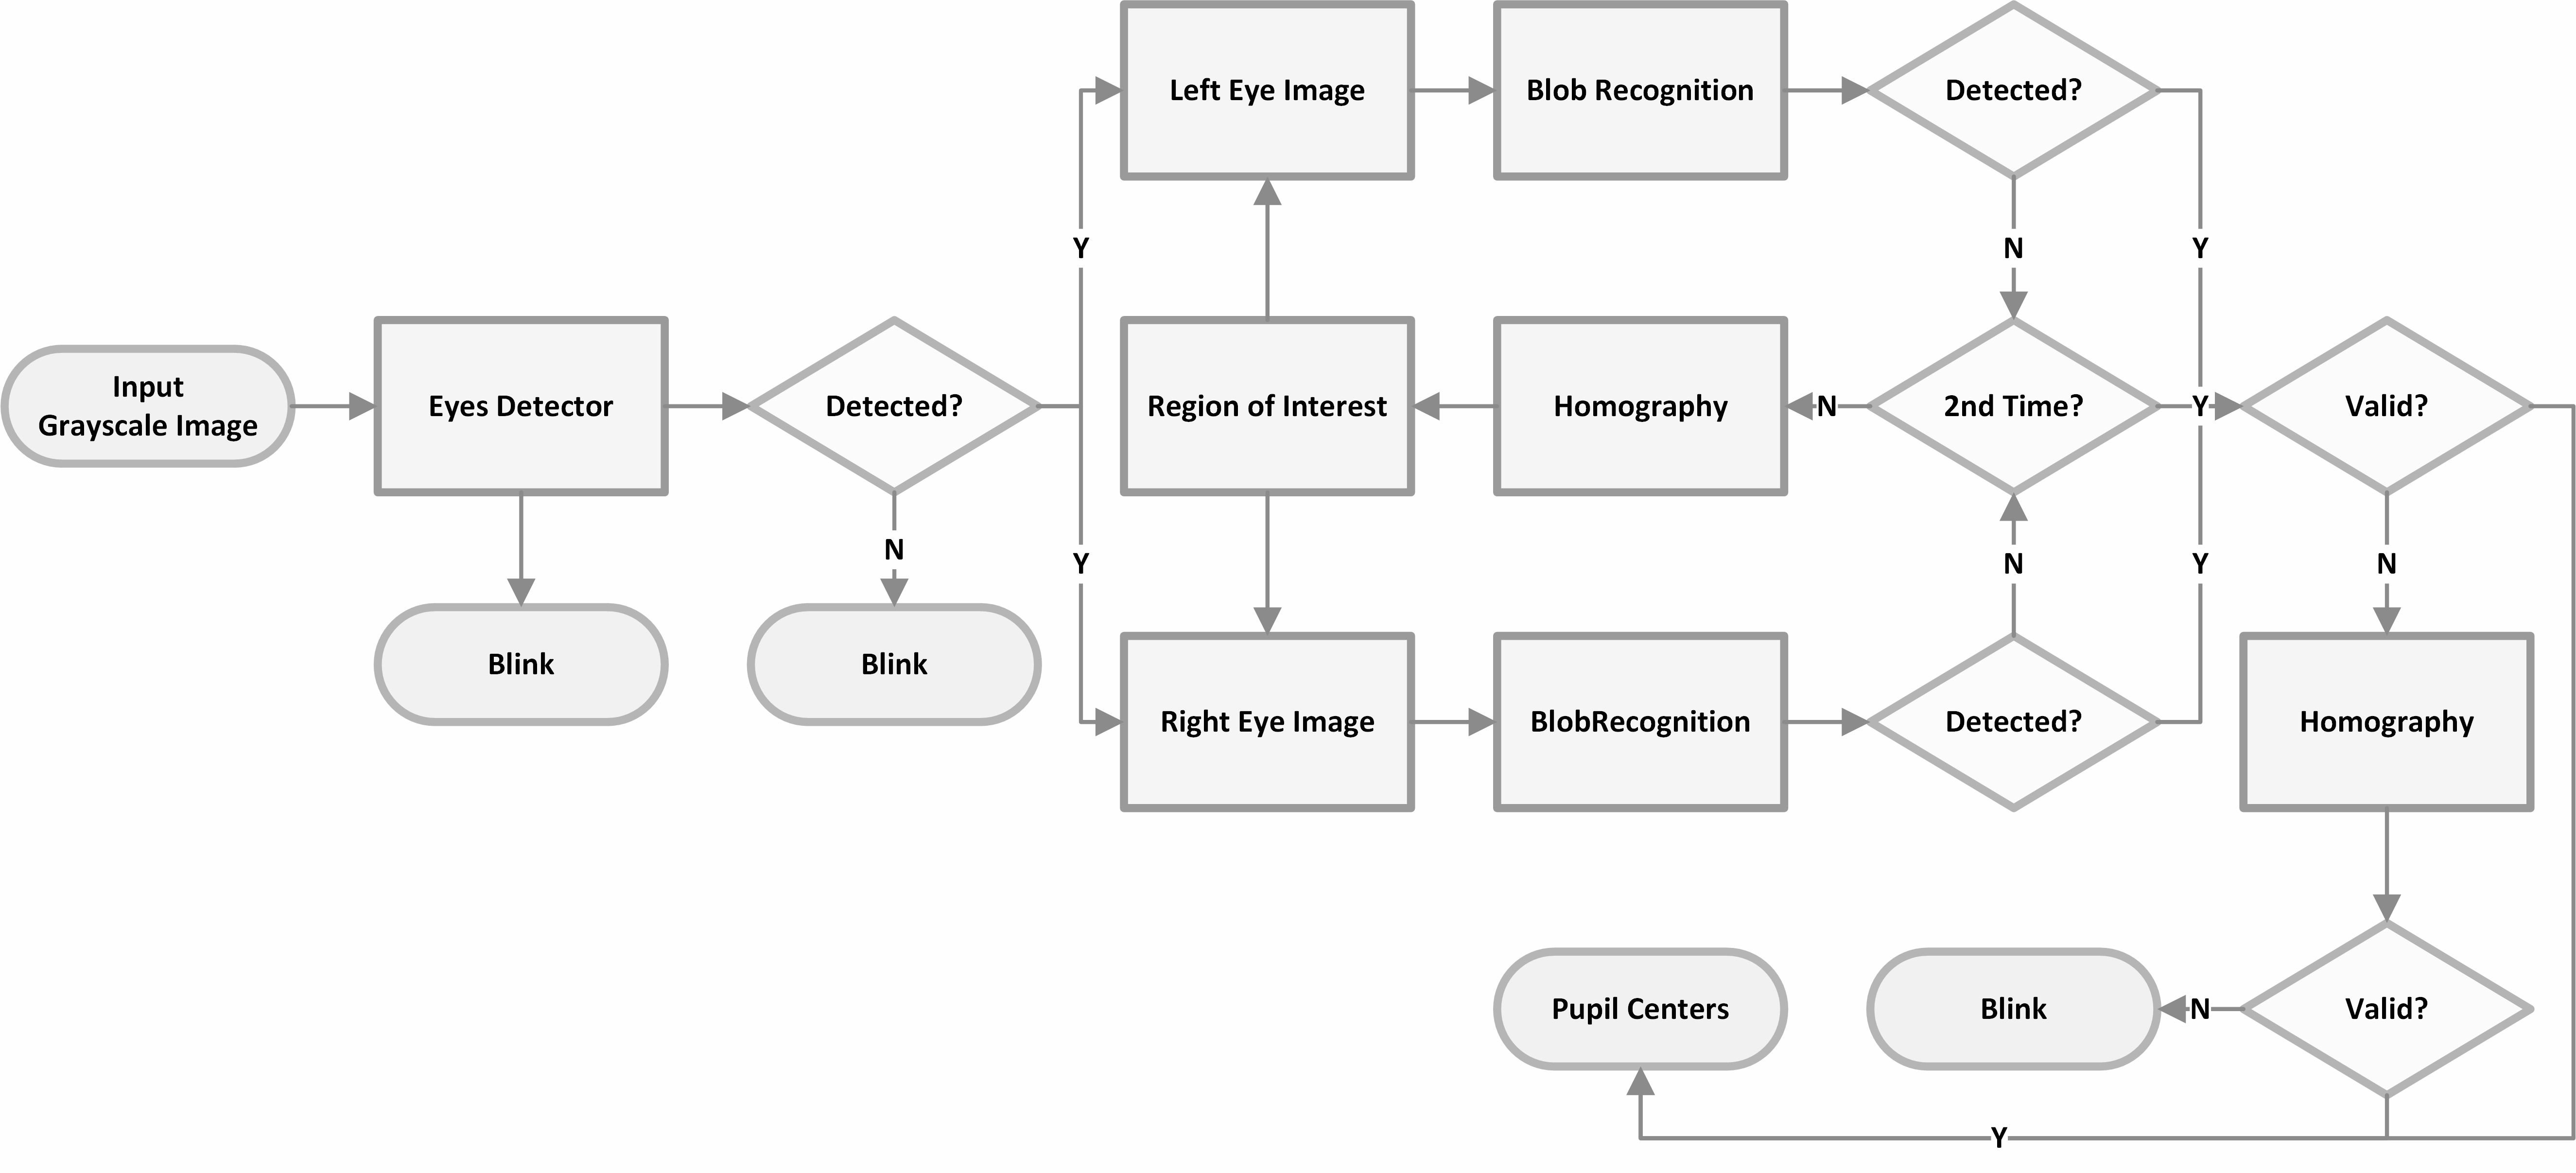
\includegraphics[width=0.8\linewidth]{flow-diagram.png}
    \caption{The proposed eye feature detector using information from both eyes}
    \label{fig:flow-diagram}
\end{figure}

On the other hand, Figure~\ref{fig:sub-figures} shows an example of a figure with subfigures. This figure includes two images side by side, each with its own caption. You can use subfigures to present related images or data together in a single figure. Figure~\ref{fig:sub-figure-a} shows an off-the-shelf head-mounted eye tracker I built during my Ph.D. research project, while Figure~\ref{fig:sub-figure-b} shows a participant of kayak experiments I performed to collect eye-tracking data of elite kayak/canoe athletes.
\begin{figure}[!ht]
    \centering
    \begin{subfigure}[b]{0.49\textwidth}
        \caption{This is the first subfigure}
        \label{fig:sub-figure-a}
        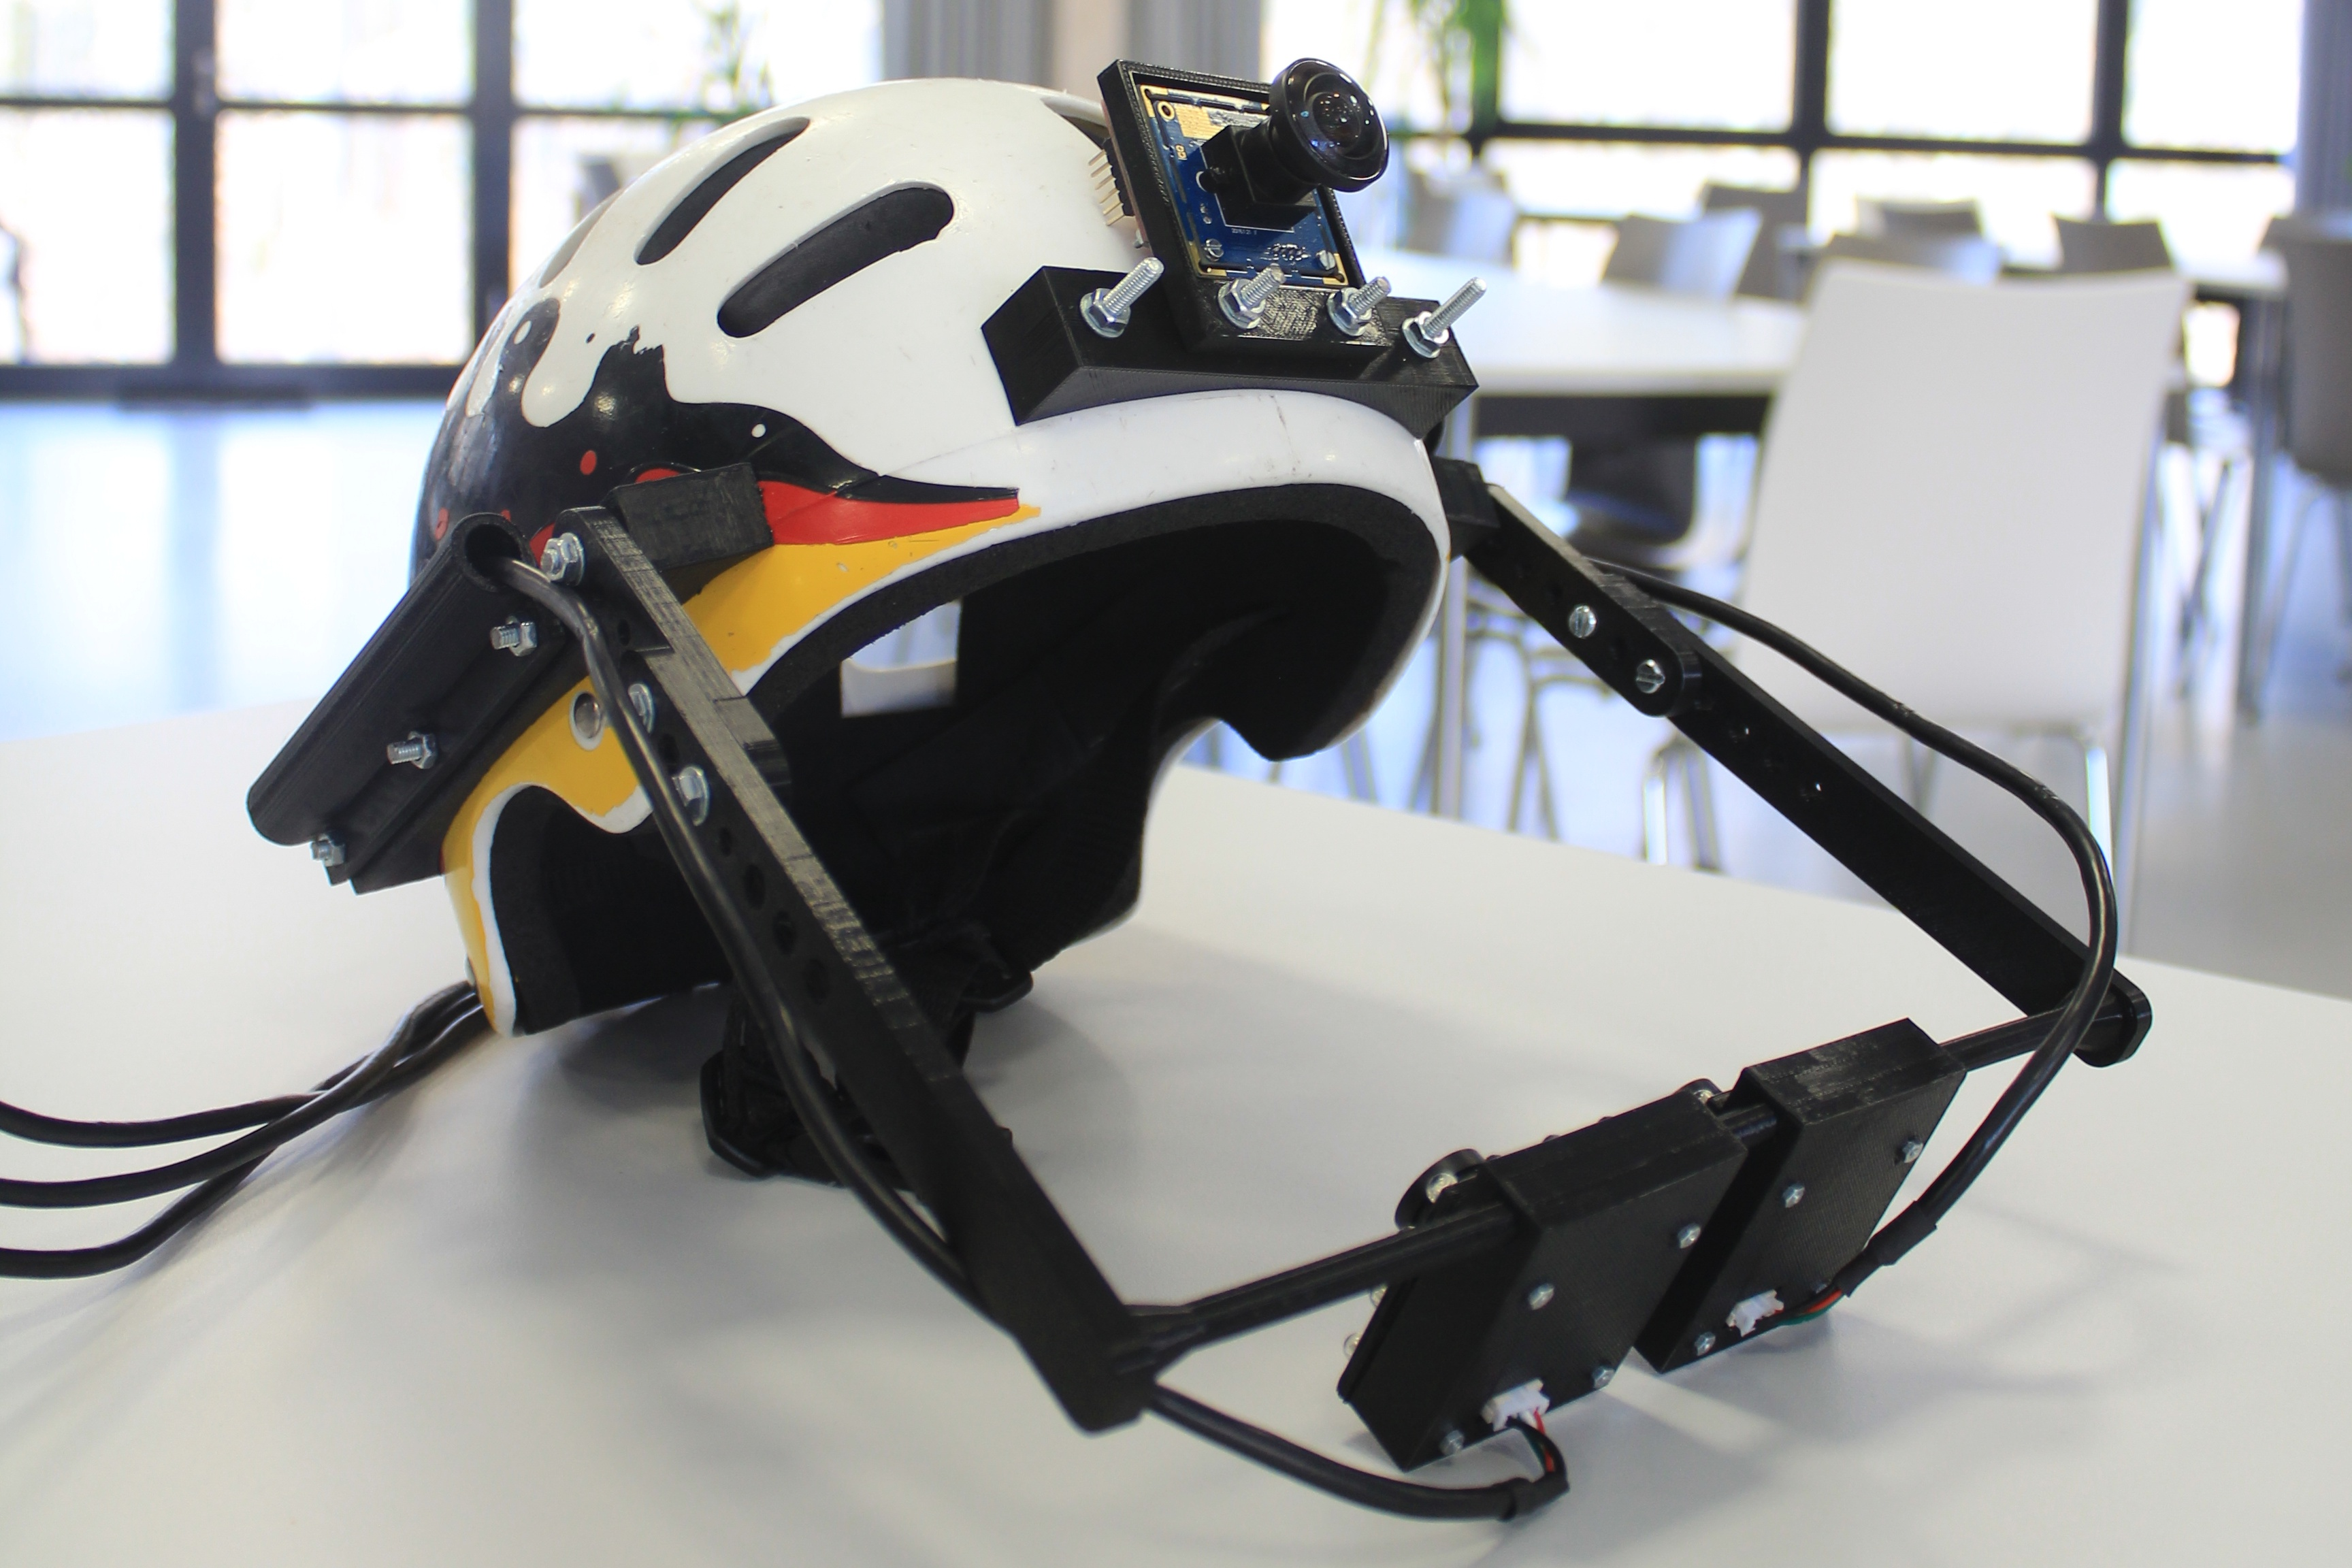
\includegraphics[width=1\linewidth]{kayak_hmet01.jpg}
    \end{subfigure}
    \begin{subfigure}[b]{0.49\textwidth}
        \caption{This is the second subfigure}
        \label{fig:sub-figure-b}
        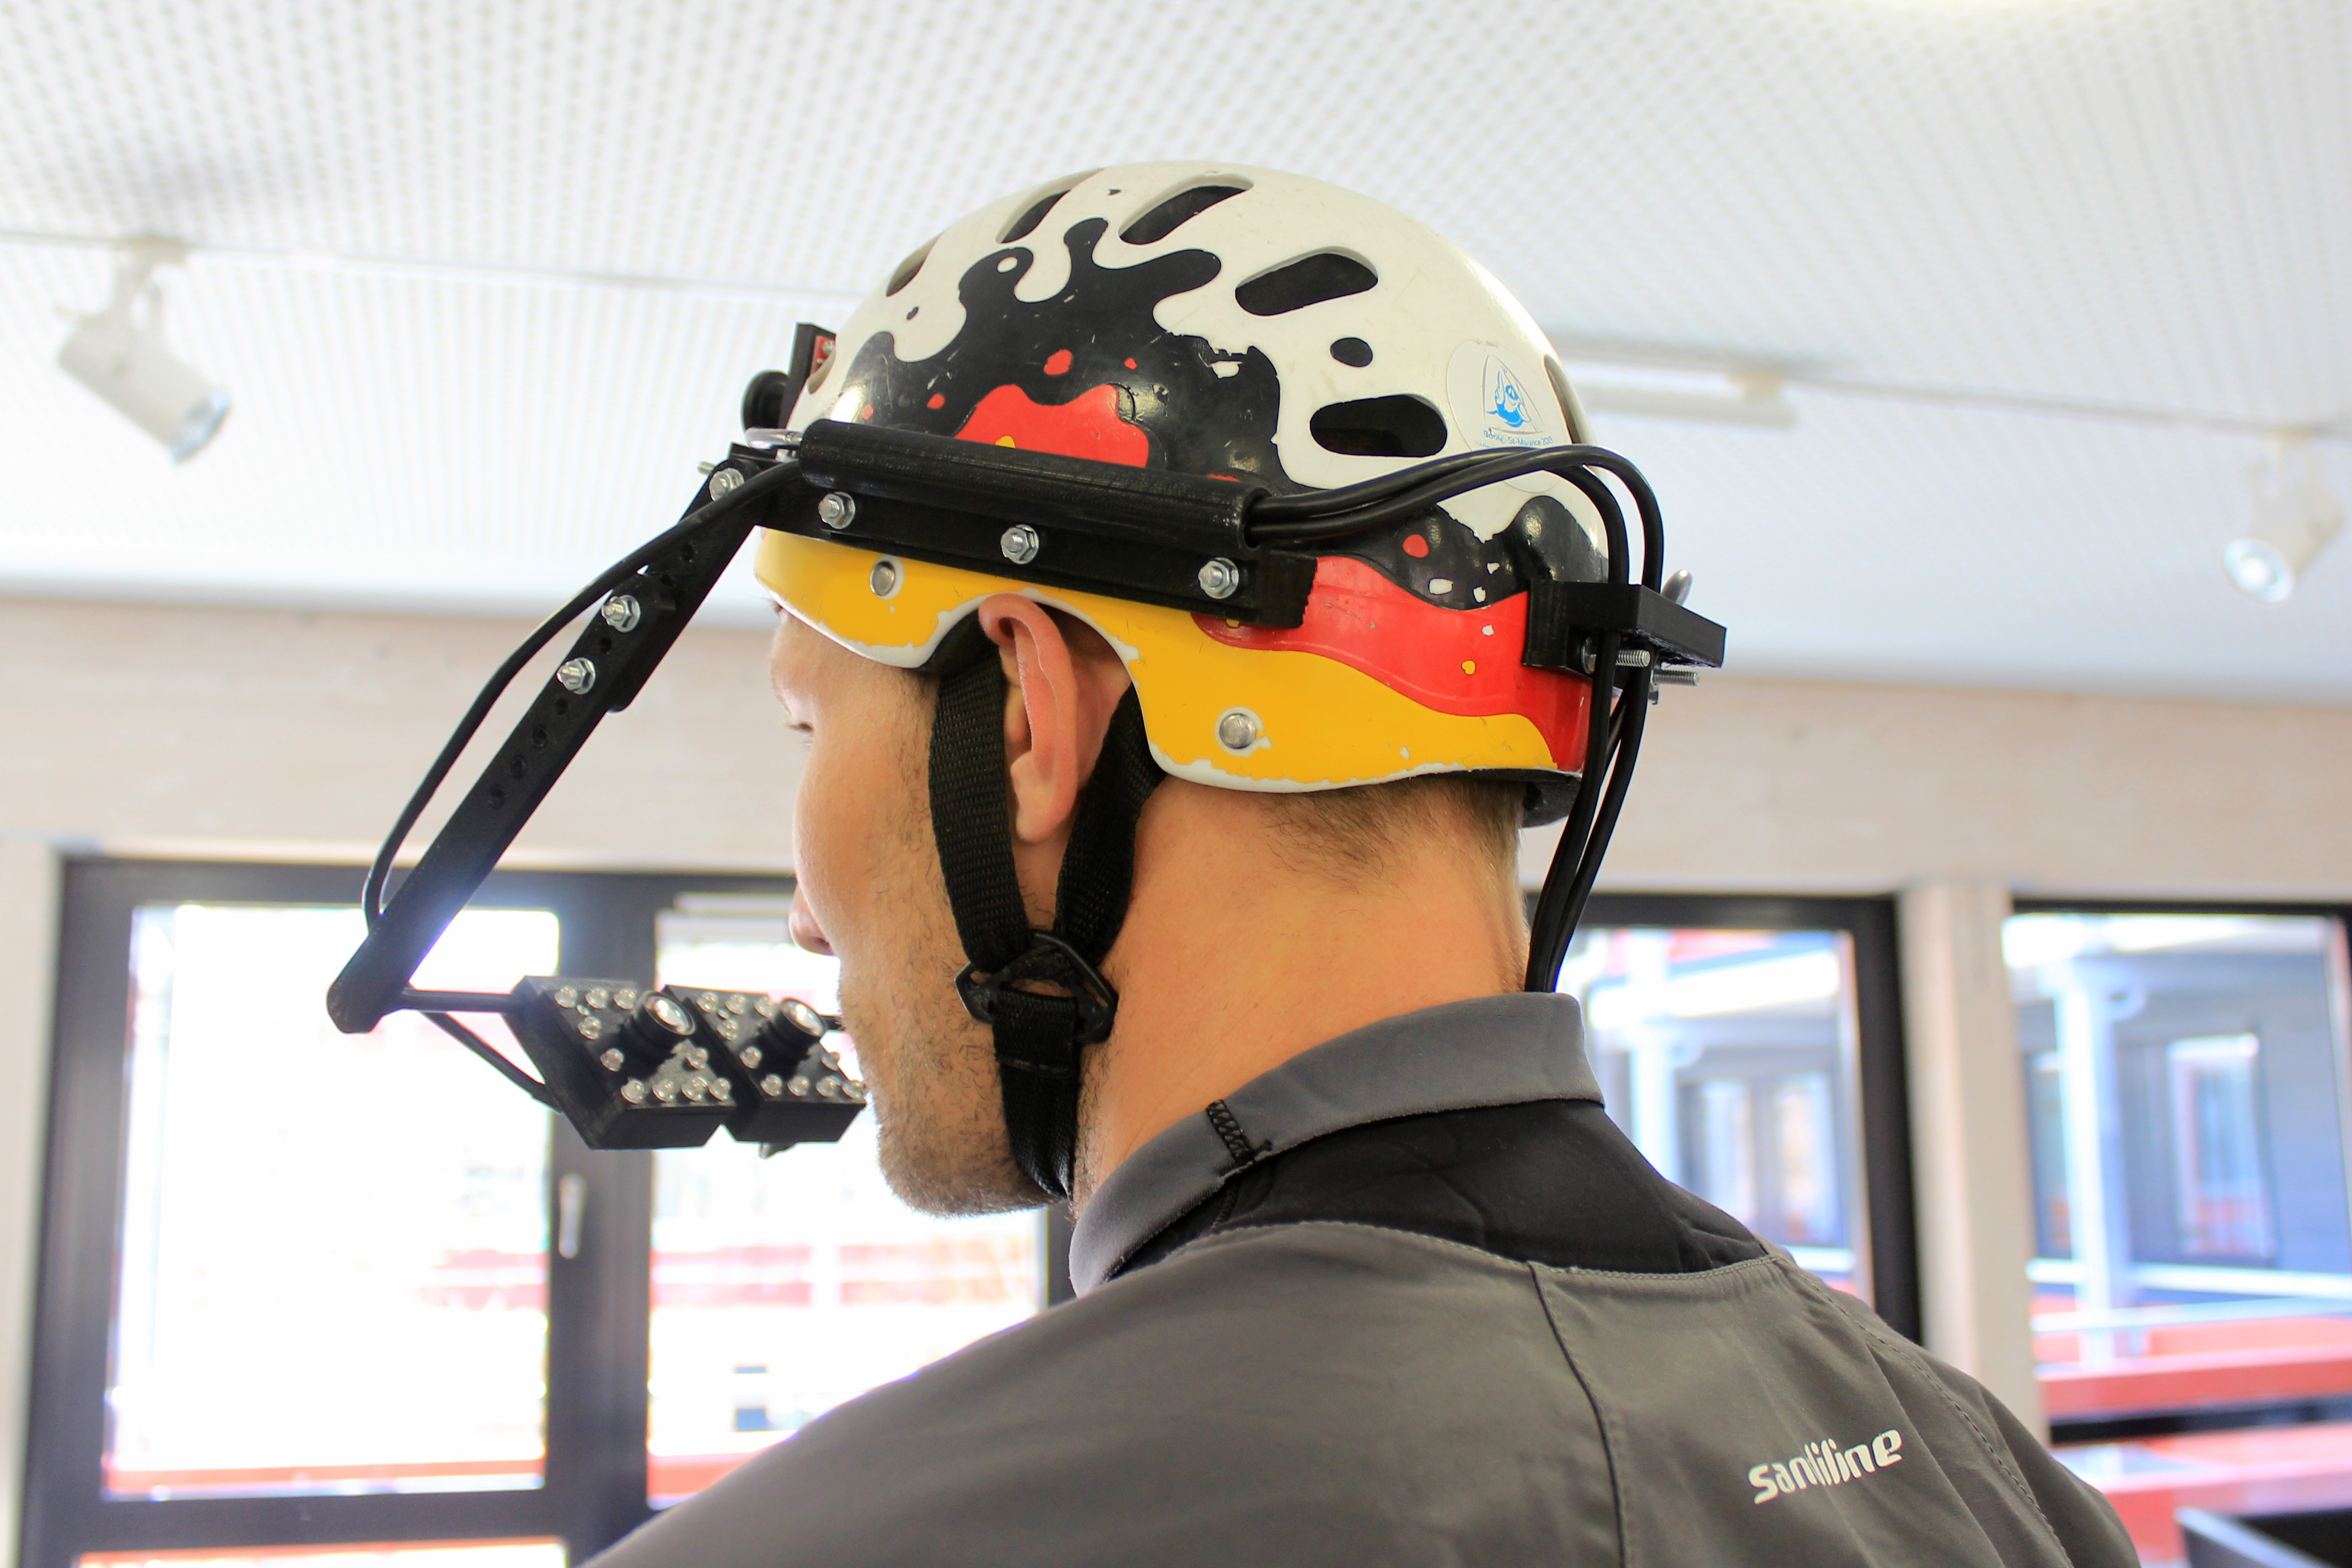
\includegraphics[width=1\linewidth]{kayak_hmet02.jpg}
    \end{subfigure}
    \caption{A head-mounted eye tracker prototype built with off-the-self hardware in a kayak helmet}
    \label{fig:sub-figures}
\end{figure}

\section{Data Collection}\label{sec:data-collection}
Provide a detailed description of how data was collected, including the datasets, tools, or systems used. Explain the sampling strategy, data sources, and data collection methods. If you conducted experiments, describe the experimental setup and procedures.

For example, you might write: ``\textit{Data was collected from 100 participants using an online survey tool. Participants were recruited through social media advertisements and were asked to complete a series of tasks related to the study. The survey included Likert scale questions, open-ended responses, and demographic information.}''

\subsection{Description of Datasets, Tools, or Systems Used}\label{subsec:datasets-tools}
Include details about the datasets, their sources, and preprocessing steps if any. Mention tools or platforms you used, such as APIs, software, or hardware. For example: ``\textit{We collected data from the Twitter API using Python scripts. The dataset consisted of 10,000 tweets related to the topic of interest. We preprocessed the data by removing duplicates and filtering out irrelevant tweets.}''

If necessary, you can include tables to present data collection details. Tables are useful for organizing large amounts of data in a structured format. For example, Table~\ref{tab:participants} shows a summary of the demographic information of the participants in the study.
\begin{center}
    \begin{threeparttable}[htbp]
        \caption{Summary of the demographic information of the participants in the study}
        \label{tab:participants}
        \begin{tabular}{cccc}
            \toprule
                \textbf{Participant ID\tnote{*}} & \textbf{Age\tnote{\textdagger}} & \textbf{Gender\tnote{\textdaggerdbl}} & \textbf{Occupation} \\
            \midrule
                1 & 25 & Female & Student \\
                2 & 30 & Male & Engineer \\
                3 & 22 & Female & Designer \\
                4 & 28 & Male & Teacher \\
                5 & 35 & Female & Scientist \\
                6 & 40 & Male & Manager \\
                7 & 27 & Female & Developer \\
                8 & 32 & Male & Analyst \\
                9 & 29 & Female & Researcher \\
                10 & 31 & Male & Consultant\tnote{\S} \\
            \bottomrule
        \end{tabular}
        \begin{tablenotes}
            \footnotesize
            \item[*] Participant ID is used to identify each participant.
            \item[\textdagger] Age is presented in years.
            \item[\textdaggerdbl] Gender is categorized.
            \item[\S] This occupation is different from the others.
        \end{tablenotes}
    \end{threeparttable}
\end{center}


In the case of a table with multiple columns, you can add the table in landscape. For example, Table~\ref{tab:participants-landscape} shows similar information as Table~\ref{tab:participants} but in a horizontal format.
\begin{landscape}
    \begin{center}
        \begin{threeparttable}[htbp]
            \caption{Demographic Information of Participants}
            \label{tab:participants-landscape}
            \begin{tabular}{cccccccc}
                \toprule
                    Participant ID & Age & Gender & Education Level & Occupation & Country & Survey Score & Comments \\
                \midrule
                    1 & 25 & Male & Bachelor's & Engineer & USA & 85 & Good \\
                    2 & 30 & Female & Master's & Scientist & UK & 90 & Excellent \\
                    3 & 22 & Non-binary & Bachelor's & Student & Canada & 75 & Average \\
                    4 & 28 & Female & PhD & Researcher & Germany & 88 & Very Good \\
                    5 & 35 & Male & High School & Technician & Australia & 80 & Good \\
                    6 & 40 & Female & Bachelor's & Manager & India & 95 & Excellent \\
                    7 & 27 & Male & Master's & Developer & Brazil & 78 & Good \\
                    8 & 32 & Female & PhD & Professor & Japan & 92 & Excellent \\
                    9 & 24 & Male & Bachelor's & Analyst & France & 82 & Good \\
                    10 & 29 & Female & Master's & Consultant & Italy & 87 & Very Good \\
                    11 & 26 & Male & Bachelor's & Designer & Spain & 83 & Good \\
                    12 & 31 & Female & Master's & Architect & Netherlands & 89 & Very Good \\
                    13 & 23 & Male & Bachelor's & Writer & Sweden & 77 & Average \\
                    14 & 34 & Female & PhD & Scientist & Switzerland & 91 & Excellent \\
                    15 & 28 & Male & High School & Technician & Norway & 79 & Good \\
                    16 & 36 & Female & Bachelor's & Engineer & Finland & 94 & Excellent \\
                    17 & 29 & Male & Master's & Developer & Denmark & 81 & Good \\
                \bottomrule
            \end{tabular}
        \end{threeparttable}
    \end{center}
\end{landscape}


If your table is too long to fit on a single page, you can use the \texttt{longtable} environment to create a table that spans multiple pages. For example, Table~\ref{tab:long-table} shows a \texttt{longtable} that continues on the next page.
\begin{longtable}{ccccc}
    \caption{Demographic information of participants (\texttt{longtable} example)}
    \label{tab:long-table} \\

    \toprule
        \textbf{ID} & \textbf{Age} & \textbf{Gender} & \textbf{Occupation} & \textbf{Country} \\
    \midrule
    \endfirsthead

    \multicolumn{5}{c}{
		\footnotesize\makebox(0,20)[c]{
			\tablename\ \thetable{} -- continued from previous page
		}
	} \\
    \toprule
        \textbf{ID} & \textbf{Age} & \textbf{Gender} & \textbf{Occupation} & \textbf{Country} \\
    \midrule
    \endhead

    \bottomrule
	\multicolumn{5}{r}{
		continues on the next page
	} \\
    \endfoot

    \bottomrule
    \multicolumn{5}{r}{
		End of \tablename\ \thetable{}
	} \\
    \endlastfoot

    1 & 25 & Male & Engineer & USA \\
    2 & 30 & Female & Scientist & UK \\
    3 & 22 & Non-binary & Student & Canada \\
    4 & 28 & Female & Designer & Australia \\
    5 & 35 & Male & Teacher & Germany \\
    6 & 27 & Female & Developer & India \\
    7 & 32 & Male & Manager & Brazil \\
    8 & 29 & Female & Nurse & Japan \\
    9 & 24 & Male & Artist & France \\
    10 & 31 & Female & Researcher & Italy \\
    11 & 26 & Male & Analyst & Spain \\
    12 & 33 & Female & Consultant & Netherlands \\
    13 & 23 & Male & Technician & Sweden \\
    14 & 34 & Female & Pharmacist & Norway \\
    15 & 28 & Male & Writer & South Africa \\
    16 & 30 & Female & Lawyer & Mexico \\
    17 & 27 & Male & Architect & China \\
    18 & 29 & Female & Chef & South Korea \\
    19 & 25 & Male & Pilot & Russia \\
    20 & 32 & Female & Accountant & Argentina \\
    21 & 28 & Male & Journalist & Egypt \\
    22 & 31 & Female & Dentist & Turkey \\
    23 & 26 & Male & Plumber & Greece \\
    24 & 33 & Female & Veterinarian & Israel \\
    25 & 29 & Male & Electrician & Portugal \\
    26 & 27 & Female & Librarian & Finland \\
    27 & 34 & Male & Carpenter & Denmark \\
    28 & 30 & Female & Biologist & Belgium \\
    29 & 25 & Male & Chemist & Austria \\
    30 & 32 & Female & Physicist & Switzerland \\
    31 & 28 & Male & Mathematician & Poland \\
    32 & 31 & Female & Economist & Hungary \\
    33 & 26 & Male & Statistician & Czech Republic \\
    34 & 33 & Female & Sociologist & Slovakia \\
    35 & 29 & Male & Psychologist & Romania \\
    36 & 27 & Female & Historian & Bulgaria \\
    37 & 34 & Male & Geologist & Croatia \\
    38 & 30 & Female & Anthropologist & Serbia \\
    39 & 25 & Male & Archaeologist & Slovenia \\
    40 & 32 & Female & Linguist & Bosnia \\
\end{longtable}


\section{Implementation Details}\label{sec:implementation-details}
Explain the algorithms, frameworks, or models you implemented. Provide a step-by-step description of how the implementation was done, including programming languages, libraries, or tools. If you developed new methods or models, describe them in detail. For example: ``\textit{We implemented a convolutional neural network using \texttt{TensorFlow} and \texttt{Keras}. The model consisted of two convolutional layers followed by two fully connected layers. We trained the model on a GPU cluster using the \texttt{Adam} optimizer with a learning rate of $0.001$. Listing~\ref{lst:cnn} shows the architecture of the CNN model implemented in Python.}''
\lstinputlisting[
    language=Python,
    belowcaptionskip=15pt,
    label={lst:cnn},
    caption={Convolutional neural network implemented in Python using TensorFlow and Keras.},
    linerange={41-50}]{codes/cnn_model.py}

\section{Evaluation Metrics}\label{sec:evaluation-metrics}
Describe the metrics used to evaluate your results. Provide mathematical definitions if applicable. For example:

The performance of the model is evaluated using accuracy, precision, recall, and F1-score, defined as:
\begin{equation}
    F1 = 2 \times \frac{\text{Precision} \times \text{Recall}}{\text{Precision} + \text{Recall}}.
\end{equation}
These metrics provide a comprehensive assessment of model performance.

\section{Ethical Considerations}\label{sec:ethical-considerations}
Discuss any ethical considerations related to your research. Explain how you addressed issues such as data privacy, informed consent, and participant anonymity. If your research involved human subjects, describe the steps you took to ensure their safety and well-being. For example: ``\textit{Participants were informed about the purpose of the study and provided written consent before participating. All data collected was anonymized to protect participant privacy. The study was approved by the Institutional Review Board (IRB) and followed ethical guidelines for research involving human subjects.}''

\section{Summary}\label{sec:methodology-summary}
Summarize the key points of the methodology chapter. Provide a brief overview of the research design, data collection methods, implementation details, evaluation metrics, and ethical considerations. This section should reinforce the importance of the methodology in ensuring the validity and reliability of your research.


% Part III: Results and Interpretation.
\part{Results and Interpretation}\label{par:results}
%
% MIT License
%
% Copyright (c) 2024 Fabricio Batista Narcizo.
%
% Permission is hereby granted, free of charge, to any person obtaining a copy
% of this software and associated documentation files (the "Software"), to deal
% in the Software without restriction, including without limitation the rights
% to use, copy, modify, merge, publish, distribute, sublicense, and/or sell
% copies of the Software, and to permit persons to whom the Software is
% furnished to do so, subject to the following conditions:
%
% The above copyright notice and this permission notice shall be included in
% all copies or substantial portions of the Software.
%
% THE SOFTWARE IS PROVIDED "AS IS", WITHOUT WARRANTY OF ANY KIND, EXPRESS OR
% IMPLIED, INCLUDING BUT NOT LIMITED TO THE WARRANTIES OF MERCHANTABILITY,
% FITNESS FOR A PARTICULAR PURPOSE AND NONINFRINGEMENT. IN NO EVENT SHALL THE
% AUTHORS OR COPYRIGHT HOLDERS BE LIABLE FOR ANY CLAIM, DAMAGES OR OTHER
% LIABILITY, WHETHER IN AN ACTION OF CONTRACT, TORT OR OTHERWISE, ARISING FROM,
% OUT OF OR IN CONNECTION WITH THE SOFTWARE OR THE USE OR OTHER DEALINGS IN THE
% SOFTWARE.
%

% Results and Analysis Chapter.
\chapter{Results and Analysis}\label{chap:results}
\lettrine[lines=3]{T}{he} results and analysis chapter presents the outcomes of your study and provides an in-depth interpretation of the findings. This chapter should be structured to highlight the connection between your research questions, the data, and the insights derived from the analysis.

Start the chapter with a brief overview of its purpose. For example: ``\textit{This chapter presents the results obtained from the experiments and analyzes them in the context of the research objectives. The findings are discussed with the support of tables, figures, and graphs, followed by a detailed interpretation of their significance.}''

\section{Data Processing and Preparation}\label{sec:data-processing}
Detail the steps taken to preprocess the data and make it suitable for analysis. Include techniques such as cleaning, normalization, or feature extraction. For example:

The data preparation involved the following steps:
\begin{enumerate}
    \item Data cleaning to handle missing values and outliers.
    \item Normalization of numerical features to ensure consistent scaling.
    \item Feature extraction using principal component analysis (PCA).
\end{enumerate}

% Example of cross-referencing.
See Chapter~\ref{chap:methodology} for details on the preprocessing tools used\footnote{This is a footnote example. Footnotes are useful for providing additional information or clarifications without disrupting the flow of the text.}.

\section{Experimental Setup}\label{sec:experimental-setup}
Explain the experimental configuration, including software, hardware, and parameters used. Provide enough detail for others to replicate your experiments. For example: ``\textit{The experiments were conducted on a system with the specifications shown in Table~\ref{tab:experimental-setup}.}''
\begin{table}[htbp]
    \centering
    \caption{Experimental setup}
    \label{tab:experimental-setup}
    \begin{tabular}{ll}
        \toprule
            \textbf{Parameter} & \textbf{Value} \\
        \midrule
            Processor          & Intel Core i7  \\
            Memory             & 16 GB          \\
            Framework          & PyTorch 2.0    \\
        \bottomrule
    \end{tabular}
\end{table}


\section{Results Presentation}\label{sec:results-presentation}
Use tables, figures, and graphs to present your results. Be sure to label and caption all visuals for easy reference. I strongly recommend using the \texttt{tikz}. For example, Figure~\ref{fig:real-data-histogram} shows the gaze-error distribution on the $Y$-axis of real eye-tracking data.
\begin{figure*}[!ht]
    \centering
    \resizebox{\textwidth}{!}{%
        \begin{tikzpicture}
	\centering
	\begin{groupplot}[
		group style={
			group size=3 by 2,
			horizontal sep=1.3cm,
			vertical sep=1.5cm
		},
		label style={font=\large},
		tick label style={font=\large}
	]

		\nextgroupplot[ybar,
			ylabel={Normalized Density},
			ymin=-0.025,
			ymax=0.25,
			xmin=-5,
			xmax=5,
			major x tick style = {opacity=0},
			xticklabel=\pgfmathprintnumber\tick$^\circ$,
			y tick label style={
				/pgf/number format/.cd,
				fixed,
				fixed zerofill,
				precision=2
			}
		]

			\node[anchor=north] at (20pt, 157pt){$H_e^s$};

			\addplot [ybar,
				fill=black!20,
				bar width=0.012\textwidth
			] plot [
				error bars/.cd,
				y dir=both,
				y explicit
			] table [
				x=bins,
				y=hist,
				y error=errors,
				col sep=comma
			] {data/01_real_01_homography_00_original.csv};

			\addplot [
				smooth,
				pattern=north east lines
			] table [
				x=x,
				y=y,
				col sep=comma,
				restrict x to domain=-0.5:0.5
			] {data/01_real_01_homography_00_original_sts.csv} \closedcycle;

			\addplot [
				color=black!50,
				smooth,
				tension=0.7,
				very thick
			] table [
				x=x,
				y=y,
				col sep=comma
			] {data/01_real_01_homography_00_original_sts.csv};

		\nextgroupplot[ybar,
			ymin=-0.025,
			ymax=0.25,
			xmin=-5,
			xmax=5,
			major x tick style = {opacity=0},
			xticklabel=\pgfmathprintnumber\tick$^\circ$,
			y tick label style={
				/pgf/number format/.cd,
				fixed,
				fixed zerofill,
				precision=2
			}
		]

			\node[anchor=north] at (20pt, 157pt){$H_e^{s+}$};

			\addplot [ybar,
				fill=black!20,
				bar width=0.012\textwidth
			] plot [
				error bars/.cd,
				y dir=both,
				y explicit
			] table [
				x=bins,
				y=hist,
				y error=errors,
				col sep=comma
			] {data/01_real_01_homography_01_camera.csv};

			\addplot [
				smooth,
				pattern=north east lines
			] table [
				x=x,
				y=y,
				col sep=comma,
				restrict x to domain=-0.5:0.5
			] {data/01_real_01_homography_01_camera_sts.csv} \closedcycle;

			\addplot [
				color=black!50,
				smooth,
				tension=0.7,
				very thick
			] table [
				x=x,
				y=y,
				col sep=comma
			] {data/01_real_01_homography_01_camera_sts.csv};

		\nextgroupplot[ybar,
			ymin=-0.025,
			ymax=0.25,
			xmin=-5,
			xmax=5,
			major x tick style = {opacity=0},
			xticklabel=\pgfmathprintnumber\tick$^\circ$,
			y tick label style={
				/pgf/number format/.cd,
				fixed,
				fixed zerofill,
				precision=2
			}
		]

			\node[anchor=north] at (20pt, 157pt){$H_e^{s*}$};

			\addplot [ybar,
				fill=black!20,
				bar width=0.012\textwidth
			] plot [
				error bars/.cd,
				y dir=both,
				y explicit
			] table [
				x=bins,
				y=hist,
				y error=errors,
				col sep=comma
			] {data/01_real_01_homography_02_distortion.csv};

			\addplot [
				smooth,
				pattern=north east lines
			] table [
				x=x,
				y=y,
				col sep=comma,
				restrict x to domain=-0.5:0.5
			] {data/01_real_01_homography_02_distortion_sts.csv} \closedcycle;

			\addplot [
				color=black!50,
				smooth,
				tension=0.7,
				very thick
			] table [
				x=x,
				y=y,
				col sep=comma
			] {data/01_real_01_homography_02_distortion_sts.csv};

		\nextgroupplot[ybar,
			xlabel=Vertical Gaze Error (\textit{deg}),
			ylabel={Normalized Density},
			ymin=-0.025,
			ymax=0.25,
			xmin=-5,
			xmax=5,
			major x tick style = {opacity=0},
			xticklabel=\pgfmathprintnumber\tick$^\circ$,
			y tick label style={
				/pgf/number format/.cd,
				fixed,
				fixed zerofill,
				precision=2
			},
			x label style={at={(0.5, -0.05)}}
		]

			\node[anchor=north] at (20pt, 157pt){$P_e^s$};

			\addplot [ybar,
				fill=black!20,
				bar width=0.012\textwidth
			] plot [
				error bars/.cd,
				y dir=both,
				y explicit
			] table [
				x=bins,
				y=hist,
				y error=errors,
				col sep=comma
			] {data/01_real_00_interpolate_00_original.csv};

			\addplot [
				smooth,
				pattern=north east lines
			] table [
				x=x,
				y=y,
				col sep=comma,
				restrict x to domain=-0.5:0.5
			] {data/01_real_00_interpolate_00_original_sts.csv} \closedcycle;

			\addplot [
				color=black!50,
				smooth,
				tension=0.7,
				very thick
			] table [
				x=x,
				y=y,
				col sep=comma
			] {data/01_real_00_interpolate_00_original_sts.csv};

		\nextgroupplot[ybar,
			xlabel=Vertical Gaze Error (\textit{deg}),
			ymin=-0.025,
			ymax=0.25,
			xmin=-5,
			xmax=5,
			major x tick style = {opacity=0},
			xticklabel=\pgfmathprintnumber\tick$^\circ$,
			y tick label style={
				/pgf/number format/.cd,
				fixed,
				fixed zerofill,
				precision=2
			},
			x label style={at={(0.5, -0.05)}},
			legend style={at={($(0,0)+(3.4cm,-2.0cm)$)},legend columns=3,fill=none,draw=black,anchor=center,align=center}
		]

			\node[anchor=north] at (20pt, 157pt){$P_e^{s+}$};

			\addplot [ybar,
				fill=black!20,
				bar width=0.012\textwidth
			] plot [
				error bars/.cd,
				y dir=both,
				y explicit
			] table [
				x=bins,
				y=hist,
				y error=errors,
				col sep=comma
			] {data/01_real_00_interpolate_01_camera.csv};
			\addlegendentry{\large{Experimental Real Data}};

			\addplot [
				smooth,
				pattern=north east lines,
				area legend
			] table [
				x=x,
				y=y,
				col sep=comma,
				restrict x to domain=-0.5:0.5
			] {data/01_real_00_interpolate_01_camera_sts.csv} \closedcycle;
			\addlegendentry{\large{High-Accuracy Range}};

			\addplot [
				color=black!50,
				smooth,
				tension=0.7,
				very thick,
				line legend
			] table [
				x=x,
				y=y,
				col sep=comma
			] {data/01_real_00_interpolate_01_camera_sts.csv};
			\addlegendentry{\large{Gaussian Fitting}};

		\nextgroupplot[ybar,
			xlabel=Vertical Gaze Error (\textit{deg}),
			ymin=-0.025,
			ymax=0.25,
			xmin=-5,
			xmax=5,
			major x tick style = {opacity=0},
			xticklabel=\pgfmathprintnumber\tick$^\circ$,
			y tick label style={
				/pgf/number format/.cd,
				fixed,
				fixed zerofill,
				precision=2
			},
			x label style={at={(0.5, -0.05)}}
		]

			\node[anchor=north] at (20pt, 157pt){$P_e^{s*}$};

			\addplot [ybar,
				fill=black!20,
				bar width=0.012\textwidth
			] plot [
				error bars/.cd,
				y dir=both,
				y explicit
			] table [
				x=bins,
				y=hist,
				y error=errors,
				col sep=comma
			] {data/01_real_00_interpolate_02_distortion.csv};

			\addplot [
				smooth,
				pattern=north east lines
			] table [
				x=x,
				y=y,
				col sep=comma,
				restrict x to domain=-0.5:0.5
			] {data/01_real_00_interpolate_02_distortion_sts.csv} \closedcycle;

			\addplot [
				color=black!50,
				smooth,
				tension=0.7,
				very thick
			] table [
				x=x,
				y=y,
				col sep=comma
			] {data/01_real_00_interpolate_02_distortion_sts.csv};

	\end{groupplot}

	\node (A) at ([yshift=0.3cm]group c1r1.north) {\large (a)};
	\node (B) at ([yshift=0.3cm]group c2r1.north) {\large (b)};
	\node (C) at ([yshift=0.3cm]group c3r1.north) {\large (c)};
	\node (D) at ([yshift=0.3cm]group c1r2.north) {\large (d)};
	\node (E) at ([yshift=0.3cm]group c2r2.north) {\large (e)};
	\node (F) at ([yshift=0.3cm]group c3r2.north) {\large (f)};

\end{tikzpicture}

    }
    \caption{Example of dynamic \texttt{tikz} plot that reads \texttt{csv} files with actual results data.}
    \label{fig:real-data-histogram}
\end{figure*}

Table~\ref{tab:real-gaussian-distribution} shows a smaller variance in the gaze-error on the $X$-axis than on $Y$-axis. The number of gaze estimations between $-0.5^\circ$ and $0.5^\circ$ increases using the methods proposed in this study~\cite{Narcizo2021}. When compared with traditional gaze estimation methods, the proposed methods (signed with \texttt{+} and \texttt{*} symbols) present a significant improvement in gaze estimation accuracy.
\begin{table}[htbp]
	\centering
  	\caption{The Gaussian PDF of real gaze estimations between $-0.5^\circ$ and $0.5^\circ$}
  	\label{tab:real-gaussian-distribution}
  	\begin{tabular}{cccc}
    	\toprule
	    	Methods & Gaze$_X$ & Gaze$_Y$ & Average \\
    	\midrule
    		$H_e^s$ & 0.50 & 0.32 & 0.41 \\
	    	$H_e^{s+}$ & 0.50 & 0.50 & 0.50 \\
    		$H_e^{s*}$ & 0.51 & 0.62 & 0.57 \\
    		$P_e^s$ & 0.47 & 0.50 & 0.49 \\
	    	$P_e^{s+}$ & 0.49 & 0.50 & 0.50 \\
    		$P_e^{s*}$ & 0.55 & 0.63 & 0.60 \\
  		\bottomrule
	\end{tabular}
\end{table}


\texttt{Tikz} is a powerful tool for creating high-quality graphics directly in \LaTeX. In my paper from 2021~\cite{Narcizo2021}, I used \texttt{tikz} to create all the figures and plots. This example reads \texttt{csv} files with the actual results data and generates a dynamic plot. The \texttt{tikz} code is available in the \texttt{tikz/real-data-histogram.tex} file and the \texttt{csv} data in the \texttt{data} folder. This file and data are the same used in the paper~\cite{Narcizo2021}.

Another good alternative for creating plots is the \texttt{pgfplots} package. This package is based on \texttt{tikz} and provides a high-level interface for creating plots. For example, Figure~\ref{fig:correlation-analysis} shows the relationships between driver characteristics (experience and age) and various driving parameters, including speeding behavior, engine speed, and vehicle speed across age groups. You can save the \texttt{Matplotlib} plots as \texttt{.pgf} files using the following Python code, just after showing the plot: \texttt{plt.savefig("pgf/co-rq-1.pgf")}.
\begin{figure}[!ht]
    \centering
    \begin{subfigure}[b]{0.49\textwidth}
        \caption{}
        \label{fig:correlation-analysis-a}
        \resizebox{\textwidth}{!}{%
            %% Creator: Matplotlib, PGF backend
%%
%% To include the figure in your LaTeX document, write
%%   \input{<filename>.pgf}
%%
%% Make sure the required packages are loaded in your preamble
%%   \usepackage{pgf}
%%
%% Also ensure that all the required font packages are loaded; for instance,
%% the lmodern package is sometimes necessary when using math font.
%%   \usepackage{lmodern}
%%
%% Figures using additional raster images can only be included by \input if
%% they are in the same directory as the main LaTeX file. For loading figures
%% from other directories you can use the `import` package
%%   \usepackage{import}
%%
%% and then include the figures with
%%   \import{<path to file>}{<filename>.pgf}
%%
%% Matplotlib used the following preamble
%%   \def\mathdefault#1{#1}
%%   \everymath=\expandafter{\the\everymath\displaystyle}
%%   
%%   \ifdefined\pdftexversion\else  % non-pdftex case.
%%     \usepackage{fontspec}
%%     \setmainfont{cmr10.ttf}[Path=\detokenize{/Users/fabricio/.miniforge3/envs/data-mining-course/lib/python3.12/site-packages/matplotlib/mpl-data/fonts/ttf/}]
%%     \setsansfont{DejaVuSans.ttf}[Path=\detokenize{/Users/fabricio/.miniforge3/envs/data-mining-course/lib/python3.12/site-packages/matplotlib/mpl-data/fonts/ttf/}]
%%     \setmonofont{DejaVuSansMono.ttf}[Path=\detokenize{/Users/fabricio/.miniforge3/envs/data-mining-course/lib/python3.12/site-packages/matplotlib/mpl-data/fonts/ttf/}]
%%   \fi
%%   \makeatletter\@ifpackageloaded{underscore}{}{\usepackage[strings]{underscore}}\makeatother
%%
\begingroup%
\makeatletter%
\begin{pgfpicture}%
\pgfpathrectangle{\pgfpointorigin}{\pgfqpoint{10.000000in}{7.000000in}}%
\pgfusepath{use as bounding box, clip}%
\begin{pgfscope}%
\pgfsetbuttcap%
\pgfsetmiterjoin%
\definecolor{currentfill}{rgb}{1.000000,1.000000,1.000000}%
\pgfsetfillcolor{currentfill}%
\pgfsetlinewidth{0.000000pt}%
\definecolor{currentstroke}{rgb}{1.000000,1.000000,1.000000}%
\pgfsetstrokecolor{currentstroke}%
\pgfsetdash{}{0pt}%
\pgfpathmoveto{\pgfqpoint{0.000000in}{0.000000in}}%
\pgfpathlineto{\pgfqpoint{10.000000in}{0.000000in}}%
\pgfpathlineto{\pgfqpoint{10.000000in}{7.000000in}}%
\pgfpathlineto{\pgfqpoint{0.000000in}{7.000000in}}%
\pgfpathlineto{\pgfqpoint{0.000000in}{0.000000in}}%
\pgfpathclose%
\pgfusepath{fill}%
\end{pgfscope}%
\begin{pgfscope}%
\pgfsetbuttcap%
\pgfsetmiterjoin%
\definecolor{currentfill}{rgb}{1.000000,1.000000,1.000000}%
\pgfsetfillcolor{currentfill}%
\pgfsetlinewidth{0.000000pt}%
\definecolor{currentstroke}{rgb}{0.000000,0.000000,0.000000}%
\pgfsetstrokecolor{currentstroke}%
\pgfsetstrokeopacity{0.000000}%
\pgfsetdash{}{0pt}%
\pgfpathmoveto{\pgfqpoint{1.250000in}{0.770000in}}%
\pgfpathlineto{\pgfqpoint{9.000000in}{0.770000in}}%
\pgfpathlineto{\pgfqpoint{9.000000in}{6.160000in}}%
\pgfpathlineto{\pgfqpoint{1.250000in}{6.160000in}}%
\pgfpathlineto{\pgfqpoint{1.250000in}{0.770000in}}%
\pgfpathclose%
\pgfusepath{fill}%
\end{pgfscope}%
\begin{pgfscope}%
\pgfpathrectangle{\pgfqpoint{1.250000in}{0.770000in}}{\pgfqpoint{7.750000in}{5.390000in}}%
\pgfusepath{clip}%
\pgfsetbuttcap%
\pgfsetroundjoin%
\pgfsetlinewidth{0.983470pt}%
\definecolor{currentstroke}{rgb}{0.000000,0.000000,0.000000}%
\pgfsetstrokecolor{currentstroke}%
\pgfsetdash{}{0pt}%
\pgfpathmoveto{\pgfqpoint{1.602273in}{4.541872in}}%
\pgfpathcurveto{\pgfqpoint{1.624829in}{4.541872in}}{\pgfqpoint{1.646464in}{4.550834in}}{\pgfqpoint{1.662413in}{4.566783in}}%
\pgfpathcurveto{\pgfqpoint{1.678363in}{4.582733in}}{\pgfqpoint{1.687324in}{4.604368in}}{\pgfqpoint{1.687324in}{4.626924in}}%
\pgfpathcurveto{\pgfqpoint{1.687324in}{4.649480in}}{\pgfqpoint{1.678363in}{4.671115in}}{\pgfqpoint{1.662413in}{4.687065in}}%
\pgfpathcurveto{\pgfqpoint{1.646464in}{4.703014in}}{\pgfqpoint{1.624829in}{4.711976in}}{\pgfqpoint{1.602273in}{4.711976in}}%
\pgfpathcurveto{\pgfqpoint{1.579717in}{4.711976in}}{\pgfqpoint{1.558082in}{4.703014in}}{\pgfqpoint{1.542132in}{4.687065in}}%
\pgfpathcurveto{\pgfqpoint{1.526183in}{4.671115in}}{\pgfqpoint{1.517221in}{4.649480in}}{\pgfqpoint{1.517221in}{4.626924in}}%
\pgfpathcurveto{\pgfqpoint{1.517221in}{4.604368in}}{\pgfqpoint{1.526183in}{4.582733in}}{\pgfqpoint{1.542132in}{4.566783in}}%
\pgfpathcurveto{\pgfqpoint{1.558082in}{4.550834in}}{\pgfqpoint{1.579717in}{4.541872in}}{\pgfqpoint{1.602273in}{4.541872in}}%
\pgfpathlineto{\pgfqpoint{1.602273in}{4.541872in}}%
\pgfpathclose%
\pgfusepath{stroke}%
\end{pgfscope}%
\begin{pgfscope}%
\pgfpathrectangle{\pgfqpoint{1.250000in}{0.770000in}}{\pgfqpoint{7.750000in}{5.390000in}}%
\pgfusepath{clip}%
\pgfsetbuttcap%
\pgfsetroundjoin%
\pgfsetlinewidth{0.983470pt}%
\definecolor{currentstroke}{rgb}{0.000000,0.000000,0.000000}%
\pgfsetstrokecolor{currentstroke}%
\pgfsetdash{}{0pt}%
\pgfpathmoveto{\pgfqpoint{1.717772in}{2.507173in}}%
\pgfpathcurveto{\pgfqpoint{1.740328in}{2.507173in}}{\pgfqpoint{1.761963in}{2.516134in}}{\pgfqpoint{1.777913in}{2.532084in}}%
\pgfpathcurveto{\pgfqpoint{1.793862in}{2.548033in}}{\pgfqpoint{1.802824in}{2.569668in}}{\pgfqpoint{1.802824in}{2.592224in}}%
\pgfpathcurveto{\pgfqpoint{1.802824in}{2.614780in}}{\pgfqpoint{1.793862in}{2.636415in}}{\pgfqpoint{1.777913in}{2.652365in}}%
\pgfpathcurveto{\pgfqpoint{1.761963in}{2.668314in}}{\pgfqpoint{1.740328in}{2.677276in}}{\pgfqpoint{1.717772in}{2.677276in}}%
\pgfpathcurveto{\pgfqpoint{1.695216in}{2.677276in}}{\pgfqpoint{1.673581in}{2.668314in}}{\pgfqpoint{1.657631in}{2.652365in}}%
\pgfpathcurveto{\pgfqpoint{1.641682in}{2.636415in}}{\pgfqpoint{1.632720in}{2.614780in}}{\pgfqpoint{1.632720in}{2.592224in}}%
\pgfpathcurveto{\pgfqpoint{1.632720in}{2.569668in}}{\pgfqpoint{1.641682in}{2.548033in}}{\pgfqpoint{1.657631in}{2.532084in}}%
\pgfpathcurveto{\pgfqpoint{1.673581in}{2.516134in}}{\pgfqpoint{1.695216in}{2.507173in}}{\pgfqpoint{1.717772in}{2.507173in}}%
\pgfpathlineto{\pgfqpoint{1.717772in}{2.507173in}}%
\pgfpathclose%
\pgfusepath{stroke}%
\end{pgfscope}%
\begin{pgfscope}%
\pgfpathrectangle{\pgfqpoint{1.250000in}{0.770000in}}{\pgfqpoint{7.750000in}{5.390000in}}%
\pgfusepath{clip}%
\pgfsetbuttcap%
\pgfsetroundjoin%
\pgfsetlinewidth{0.983470pt}%
\definecolor{currentstroke}{rgb}{0.000000,0.000000,0.000000}%
\pgfsetstrokecolor{currentstroke}%
\pgfsetdash{}{0pt}%
\pgfpathmoveto{\pgfqpoint{1.833271in}{3.556152in}}%
\pgfpathcurveto{\pgfqpoint{1.855827in}{3.556152in}}{\pgfqpoint{1.877462in}{3.565114in}}{\pgfqpoint{1.893412in}{3.581063in}}%
\pgfpathcurveto{\pgfqpoint{1.909361in}{3.597013in}}{\pgfqpoint{1.918323in}{3.618648in}}{\pgfqpoint{1.918323in}{3.641204in}}%
\pgfpathcurveto{\pgfqpoint{1.918323in}{3.663760in}}{\pgfqpoint{1.909361in}{3.685395in}}{\pgfqpoint{1.893412in}{3.701345in}}%
\pgfpathcurveto{\pgfqpoint{1.877462in}{3.717294in}}{\pgfqpoint{1.855827in}{3.726256in}}{\pgfqpoint{1.833271in}{3.726256in}}%
\pgfpathcurveto{\pgfqpoint{1.810715in}{3.726256in}}{\pgfqpoint{1.789080in}{3.717294in}}{\pgfqpoint{1.773131in}{3.701345in}}%
\pgfpathcurveto{\pgfqpoint{1.757181in}{3.685395in}}{\pgfqpoint{1.748220in}{3.663760in}}{\pgfqpoint{1.748220in}{3.641204in}}%
\pgfpathcurveto{\pgfqpoint{1.748220in}{3.618648in}}{\pgfqpoint{1.757181in}{3.597013in}}{\pgfqpoint{1.773131in}{3.581063in}}%
\pgfpathcurveto{\pgfqpoint{1.789080in}{3.565114in}}{\pgfqpoint{1.810715in}{3.556152in}}{\pgfqpoint{1.833271in}{3.556152in}}%
\pgfpathlineto{\pgfqpoint{1.833271in}{3.556152in}}%
\pgfpathclose%
\pgfusepath{stroke}%
\end{pgfscope}%
\begin{pgfscope}%
\pgfpathrectangle{\pgfqpoint{1.250000in}{0.770000in}}{\pgfqpoint{7.750000in}{5.390000in}}%
\pgfusepath{clip}%
\pgfsetbuttcap%
\pgfsetroundjoin%
\pgfsetlinewidth{0.983470pt}%
\definecolor{currentstroke}{rgb}{0.000000,0.000000,0.000000}%
\pgfsetstrokecolor{currentstroke}%
\pgfsetdash{}{0pt}%
\pgfpathmoveto{\pgfqpoint{1.948770in}{5.021249in}}%
\pgfpathcurveto{\pgfqpoint{1.971326in}{5.021249in}}{\pgfqpoint{1.992962in}{5.030211in}}{\pgfqpoint{2.008911in}{5.046160in}}%
\pgfpathcurveto{\pgfqpoint{2.024861in}{5.062110in}}{\pgfqpoint{2.033822in}{5.083745in}}{\pgfqpoint{2.033822in}{5.106301in}}%
\pgfpathcurveto{\pgfqpoint{2.033822in}{5.128857in}}{\pgfqpoint{2.024861in}{5.150492in}}{\pgfqpoint{2.008911in}{5.166441in}}%
\pgfpathcurveto{\pgfqpoint{1.992962in}{5.182391in}}{\pgfqpoint{1.971326in}{5.191353in}}{\pgfqpoint{1.948770in}{5.191353in}}%
\pgfpathcurveto{\pgfqpoint{1.926215in}{5.191353in}}{\pgfqpoint{1.904579in}{5.182391in}}{\pgfqpoint{1.888630in}{5.166441in}}%
\pgfpathcurveto{\pgfqpoint{1.872680in}{5.150492in}}{\pgfqpoint{1.863719in}{5.128857in}}{\pgfqpoint{1.863719in}{5.106301in}}%
\pgfpathcurveto{\pgfqpoint{1.863719in}{5.083745in}}{\pgfqpoint{1.872680in}{5.062110in}}{\pgfqpoint{1.888630in}{5.046160in}}%
\pgfpathcurveto{\pgfqpoint{1.904579in}{5.030211in}}{\pgfqpoint{1.926215in}{5.021249in}}{\pgfqpoint{1.948770in}{5.021249in}}%
\pgfpathlineto{\pgfqpoint{1.948770in}{5.021249in}}%
\pgfpathclose%
\pgfusepath{stroke}%
\end{pgfscope}%
\begin{pgfscope}%
\pgfpathrectangle{\pgfqpoint{1.250000in}{0.770000in}}{\pgfqpoint{7.750000in}{5.390000in}}%
\pgfusepath{clip}%
\pgfsetbuttcap%
\pgfsetroundjoin%
\pgfsetlinewidth{0.983470pt}%
\definecolor{currentstroke}{rgb}{0.000000,0.000000,0.000000}%
\pgfsetstrokecolor{currentstroke}%
\pgfsetdash{}{0pt}%
\pgfpathmoveto{\pgfqpoint{2.064270in}{2.824438in}}%
\pgfpathcurveto{\pgfqpoint{2.086826in}{2.824438in}}{\pgfqpoint{2.108461in}{2.833399in}}{\pgfqpoint{2.124410in}{2.849349in}}%
\pgfpathcurveto{\pgfqpoint{2.140360in}{2.865298in}}{\pgfqpoint{2.149321in}{2.886934in}}{\pgfqpoint{2.149321in}{2.909490in}}%
\pgfpathcurveto{\pgfqpoint{2.149321in}{2.932046in}}{\pgfqpoint{2.140360in}{2.953681in}}{\pgfqpoint{2.124410in}{2.969630in}}%
\pgfpathcurveto{\pgfqpoint{2.108461in}{2.985580in}}{\pgfqpoint{2.086826in}{2.994541in}}{\pgfqpoint{2.064270in}{2.994541in}}%
\pgfpathcurveto{\pgfqpoint{2.041714in}{2.994541in}}{\pgfqpoint{2.020079in}{2.985580in}}{\pgfqpoint{2.004129in}{2.969630in}}%
\pgfpathcurveto{\pgfqpoint{1.988180in}{2.953681in}}{\pgfqpoint{1.979218in}{2.932046in}}{\pgfqpoint{1.979218in}{2.909490in}}%
\pgfpathcurveto{\pgfqpoint{1.979218in}{2.886934in}}{\pgfqpoint{1.988180in}{2.865298in}}{\pgfqpoint{2.004129in}{2.849349in}}%
\pgfpathcurveto{\pgfqpoint{2.020079in}{2.833399in}}{\pgfqpoint{2.041714in}{2.824438in}}{\pgfqpoint{2.064270in}{2.824438in}}%
\pgfpathlineto{\pgfqpoint{2.064270in}{2.824438in}}%
\pgfpathclose%
\pgfusepath{stroke}%
\end{pgfscope}%
\begin{pgfscope}%
\pgfpathrectangle{\pgfqpoint{1.250000in}{0.770000in}}{\pgfqpoint{7.750000in}{5.390000in}}%
\pgfusepath{clip}%
\pgfsetbuttcap%
\pgfsetroundjoin%
\pgfsetlinewidth{0.983470pt}%
\definecolor{currentstroke}{rgb}{0.000000,0.000000,0.000000}%
\pgfsetstrokecolor{currentstroke}%
\pgfsetdash{}{0pt}%
\pgfpathmoveto{\pgfqpoint{2.526267in}{5.829948in}}%
\pgfpathcurveto{\pgfqpoint{2.548823in}{5.829948in}}{\pgfqpoint{2.570458in}{5.838910in}}{\pgfqpoint{2.586407in}{5.854859in}}%
\pgfpathcurveto{\pgfqpoint{2.602357in}{5.870809in}}{\pgfqpoint{2.611318in}{5.892444in}}{\pgfqpoint{2.611318in}{5.915000in}}%
\pgfpathcurveto{\pgfqpoint{2.611318in}{5.937556in}}{\pgfqpoint{2.602357in}{5.959191in}}{\pgfqpoint{2.586407in}{5.975141in}}%
\pgfpathcurveto{\pgfqpoint{2.570458in}{5.991090in}}{\pgfqpoint{2.548823in}{6.000052in}}{\pgfqpoint{2.526267in}{6.000052in}}%
\pgfpathcurveto{\pgfqpoint{2.503711in}{6.000052in}}{\pgfqpoint{2.482076in}{5.991090in}}{\pgfqpoint{2.466126in}{5.975141in}}%
\pgfpathcurveto{\pgfqpoint{2.450177in}{5.959191in}}{\pgfqpoint{2.441215in}{5.937556in}}{\pgfqpoint{2.441215in}{5.915000in}}%
\pgfpathcurveto{\pgfqpoint{2.441215in}{5.892444in}}{\pgfqpoint{2.450177in}{5.870809in}}{\pgfqpoint{2.466126in}{5.854859in}}%
\pgfpathcurveto{\pgfqpoint{2.482076in}{5.838910in}}{\pgfqpoint{2.503711in}{5.829948in}}{\pgfqpoint{2.526267in}{5.829948in}}%
\pgfpathlineto{\pgfqpoint{2.526267in}{5.829948in}}%
\pgfpathclose%
\pgfusepath{stroke}%
\end{pgfscope}%
\begin{pgfscope}%
\pgfpathrectangle{\pgfqpoint{1.250000in}{0.770000in}}{\pgfqpoint{7.750000in}{5.390000in}}%
\pgfusepath{clip}%
\pgfsetbuttcap%
\pgfsetroundjoin%
\pgfsetlinewidth{0.983470pt}%
\definecolor{currentstroke}{rgb}{0.000000,0.000000,0.000000}%
\pgfsetstrokecolor{currentstroke}%
\pgfsetdash{}{0pt}%
\pgfpathmoveto{\pgfqpoint{2.757265in}{3.654826in}}%
\pgfpathcurveto{\pgfqpoint{2.779821in}{3.654826in}}{\pgfqpoint{2.801456in}{3.663788in}}{\pgfqpoint{2.817406in}{3.679737in}}%
\pgfpathcurveto{\pgfqpoint{2.833355in}{3.695687in}}{\pgfqpoint{2.842317in}{3.717322in}}{\pgfqpoint{2.842317in}{3.739878in}}%
\pgfpathcurveto{\pgfqpoint{2.842317in}{3.762434in}}{\pgfqpoint{2.833355in}{3.784069in}}{\pgfqpoint{2.817406in}{3.800019in}}%
\pgfpathcurveto{\pgfqpoint{2.801456in}{3.815968in}}{\pgfqpoint{2.779821in}{3.824930in}}{\pgfqpoint{2.757265in}{3.824930in}}%
\pgfpathcurveto{\pgfqpoint{2.734709in}{3.824930in}}{\pgfqpoint{2.713074in}{3.815968in}}{\pgfqpoint{2.697125in}{3.800019in}}%
\pgfpathcurveto{\pgfqpoint{2.681175in}{3.784069in}}{\pgfqpoint{2.672214in}{3.762434in}}{\pgfqpoint{2.672214in}{3.739878in}}%
\pgfpathcurveto{\pgfqpoint{2.672214in}{3.717322in}}{\pgfqpoint{2.681175in}{3.695687in}}{\pgfqpoint{2.697125in}{3.679737in}}%
\pgfpathcurveto{\pgfqpoint{2.713074in}{3.663788in}}{\pgfqpoint{2.734709in}{3.654826in}}{\pgfqpoint{2.757265in}{3.654826in}}%
\pgfpathlineto{\pgfqpoint{2.757265in}{3.654826in}}%
\pgfpathclose%
\pgfusepath{stroke}%
\end{pgfscope}%
\begin{pgfscope}%
\pgfpathrectangle{\pgfqpoint{1.250000in}{0.770000in}}{\pgfqpoint{7.750000in}{5.390000in}}%
\pgfusepath{clip}%
\pgfsetbuttcap%
\pgfsetroundjoin%
\pgfsetlinewidth{0.983470pt}%
\definecolor{currentstroke}{rgb}{0.000000,0.000000,0.000000}%
\pgfsetstrokecolor{currentstroke}%
\pgfsetdash{}{0pt}%
\pgfpathmoveto{\pgfqpoint{4.489754in}{3.056007in}}%
\pgfpathcurveto{\pgfqpoint{4.512310in}{3.056007in}}{\pgfqpoint{4.533945in}{3.064969in}}{\pgfqpoint{4.549895in}{3.080918in}}%
\pgfpathcurveto{\pgfqpoint{4.565844in}{3.096868in}}{\pgfqpoint{4.574806in}{3.118503in}}{\pgfqpoint{4.574806in}{3.141059in}}%
\pgfpathcurveto{\pgfqpoint{4.574806in}{3.163615in}}{\pgfqpoint{4.565844in}{3.185250in}}{\pgfqpoint{4.549895in}{3.201200in}}%
\pgfpathcurveto{\pgfqpoint{4.533945in}{3.217149in}}{\pgfqpoint{4.512310in}{3.226111in}}{\pgfqpoint{4.489754in}{3.226111in}}%
\pgfpathcurveto{\pgfqpoint{4.467198in}{3.226111in}}{\pgfqpoint{4.445563in}{3.217149in}}{\pgfqpoint{4.429613in}{3.201200in}}%
\pgfpathcurveto{\pgfqpoint{4.413664in}{3.185250in}}{\pgfqpoint{4.404702in}{3.163615in}}{\pgfqpoint{4.404702in}{3.141059in}}%
\pgfpathcurveto{\pgfqpoint{4.404702in}{3.118503in}}{\pgfqpoint{4.413664in}{3.096868in}}{\pgfqpoint{4.429613in}{3.080918in}}%
\pgfpathcurveto{\pgfqpoint{4.445563in}{3.064969in}}{\pgfqpoint{4.467198in}{3.056007in}}{\pgfqpoint{4.489754in}{3.056007in}}%
\pgfpathlineto{\pgfqpoint{4.489754in}{3.056007in}}%
\pgfpathclose%
\pgfusepath{stroke}%
\end{pgfscope}%
\begin{pgfscope}%
\pgfpathrectangle{\pgfqpoint{1.250000in}{0.770000in}}{\pgfqpoint{7.750000in}{5.390000in}}%
\pgfusepath{clip}%
\pgfsetbuttcap%
\pgfsetroundjoin%
\pgfsetlinewidth{0.983470pt}%
\definecolor{currentstroke}{rgb}{0.000000,0.000000,0.000000}%
\pgfsetstrokecolor{currentstroke}%
\pgfsetdash{}{0pt}%
\pgfpathmoveto{\pgfqpoint{4.951751in}{3.599054in}}%
\pgfpathcurveto{\pgfqpoint{4.974307in}{3.599054in}}{\pgfqpoint{4.995942in}{3.608016in}}{\pgfqpoint{5.011892in}{3.623965in}}%
\pgfpathcurveto{\pgfqpoint{5.027841in}{3.639915in}}{\pgfqpoint{5.036803in}{3.661550in}}{\pgfqpoint{5.036803in}{3.684106in}}%
\pgfpathcurveto{\pgfqpoint{5.036803in}{3.706662in}}{\pgfqpoint{5.027841in}{3.728297in}}{\pgfqpoint{5.011892in}{3.744246in}}%
\pgfpathcurveto{\pgfqpoint{4.995942in}{3.760196in}}{\pgfqpoint{4.974307in}{3.769157in}}{\pgfqpoint{4.951751in}{3.769157in}}%
\pgfpathcurveto{\pgfqpoint{4.929195in}{3.769157in}}{\pgfqpoint{4.907560in}{3.760196in}}{\pgfqpoint{4.891610in}{3.744246in}}%
\pgfpathcurveto{\pgfqpoint{4.875661in}{3.728297in}}{\pgfqpoint{4.866699in}{3.706662in}}{\pgfqpoint{4.866699in}{3.684106in}}%
\pgfpathcurveto{\pgfqpoint{4.866699in}{3.661550in}}{\pgfqpoint{4.875661in}{3.639915in}}{\pgfqpoint{4.891610in}{3.623965in}}%
\pgfpathcurveto{\pgfqpoint{4.907560in}{3.608016in}}{\pgfqpoint{4.929195in}{3.599054in}}{\pgfqpoint{4.951751in}{3.599054in}}%
\pgfpathlineto{\pgfqpoint{4.951751in}{3.599054in}}%
\pgfpathclose%
\pgfusepath{stroke}%
\end{pgfscope}%
\begin{pgfscope}%
\pgfpathrectangle{\pgfqpoint{1.250000in}{0.770000in}}{\pgfqpoint{7.750000in}{5.390000in}}%
\pgfusepath{clip}%
\pgfsetbuttcap%
\pgfsetroundjoin%
\pgfsetlinewidth{0.983470pt}%
\definecolor{currentstroke}{rgb}{0.000000,0.000000,0.000000}%
\pgfsetstrokecolor{currentstroke}%
\pgfsetdash{}{0pt}%
\pgfpathmoveto{\pgfqpoint{5.182750in}{1.797178in}}%
\pgfpathcurveto{\pgfqpoint{5.205306in}{1.797178in}}{\pgfqpoint{5.226941in}{1.806139in}}{\pgfqpoint{5.242890in}{1.822089in}}%
\pgfpathcurveto{\pgfqpoint{5.258840in}{1.838038in}}{\pgfqpoint{5.267801in}{1.859674in}}{\pgfqpoint{5.267801in}{1.882230in}}%
\pgfpathcurveto{\pgfqpoint{5.267801in}{1.904786in}}{\pgfqpoint{5.258840in}{1.926421in}}{\pgfqpoint{5.242890in}{1.942370in}}%
\pgfpathcurveto{\pgfqpoint{5.226941in}{1.958320in}}{\pgfqpoint{5.205306in}{1.967281in}}{\pgfqpoint{5.182750in}{1.967281in}}%
\pgfpathcurveto{\pgfqpoint{5.160194in}{1.967281in}}{\pgfqpoint{5.138558in}{1.958320in}}{\pgfqpoint{5.122609in}{1.942370in}}%
\pgfpathcurveto{\pgfqpoint{5.106659in}{1.926421in}}{\pgfqpoint{5.097698in}{1.904786in}}{\pgfqpoint{5.097698in}{1.882230in}}%
\pgfpathcurveto{\pgfqpoint{5.097698in}{1.859674in}}{\pgfqpoint{5.106659in}{1.838038in}}{\pgfqpoint{5.122609in}{1.822089in}}%
\pgfpathcurveto{\pgfqpoint{5.138558in}{1.806139in}}{\pgfqpoint{5.160194in}{1.797178in}}{\pgfqpoint{5.182750in}{1.797178in}}%
\pgfpathlineto{\pgfqpoint{5.182750in}{1.797178in}}%
\pgfpathclose%
\pgfusepath{stroke}%
\end{pgfscope}%
\begin{pgfscope}%
\pgfpathrectangle{\pgfqpoint{1.250000in}{0.770000in}}{\pgfqpoint{7.750000in}{5.390000in}}%
\pgfusepath{clip}%
\pgfsetbuttcap%
\pgfsetroundjoin%
\pgfsetlinewidth{0.983470pt}%
\definecolor{currentstroke}{rgb}{0.000000,0.000000,0.000000}%
\pgfsetstrokecolor{currentstroke}%
\pgfsetdash{}{0pt}%
\pgfpathmoveto{\pgfqpoint{5.413748in}{3.277290in}}%
\pgfpathcurveto{\pgfqpoint{5.436304in}{3.277290in}}{\pgfqpoint{5.457939in}{3.286252in}}{\pgfqpoint{5.473889in}{3.302201in}}%
\pgfpathcurveto{\pgfqpoint{5.489838in}{3.318151in}}{\pgfqpoint{5.498800in}{3.339786in}}{\pgfqpoint{5.498800in}{3.362342in}}%
\pgfpathcurveto{\pgfqpoint{5.498800in}{3.384898in}}{\pgfqpoint{5.489838in}{3.406533in}}{\pgfqpoint{5.473889in}{3.422483in}}%
\pgfpathcurveto{\pgfqpoint{5.457939in}{3.438432in}}{\pgfqpoint{5.436304in}{3.447394in}}{\pgfqpoint{5.413748in}{3.447394in}}%
\pgfpathcurveto{\pgfqpoint{5.391192in}{3.447394in}}{\pgfqpoint{5.369557in}{3.438432in}}{\pgfqpoint{5.353607in}{3.422483in}}%
\pgfpathcurveto{\pgfqpoint{5.337658in}{3.406533in}}{\pgfqpoint{5.328696in}{3.384898in}}{\pgfqpoint{5.328696in}{3.362342in}}%
\pgfpathcurveto{\pgfqpoint{5.328696in}{3.339786in}}{\pgfqpoint{5.337658in}{3.318151in}}{\pgfqpoint{5.353607in}{3.302201in}}%
\pgfpathcurveto{\pgfqpoint{5.369557in}{3.286252in}}{\pgfqpoint{5.391192in}{3.277290in}}{\pgfqpoint{5.413748in}{3.277290in}}%
\pgfpathlineto{\pgfqpoint{5.413748in}{3.277290in}}%
\pgfpathclose%
\pgfusepath{stroke}%
\end{pgfscope}%
\begin{pgfscope}%
\pgfpathrectangle{\pgfqpoint{1.250000in}{0.770000in}}{\pgfqpoint{7.750000in}{5.390000in}}%
\pgfusepath{clip}%
\pgfsetbuttcap%
\pgfsetroundjoin%
\pgfsetlinewidth{0.983470pt}%
\definecolor{currentstroke}{rgb}{0.000000,0.000000,0.000000}%
\pgfsetstrokecolor{currentstroke}%
\pgfsetdash{}{0pt}%
\pgfpathmoveto{\pgfqpoint{5.644747in}{2.448749in}}%
\pgfpathcurveto{\pgfqpoint{5.667303in}{2.448749in}}{\pgfqpoint{5.688938in}{2.457711in}}{\pgfqpoint{5.704887in}{2.473660in}}%
\pgfpathcurveto{\pgfqpoint{5.720837in}{2.489610in}}{\pgfqpoint{5.729798in}{2.511245in}}{\pgfqpoint{5.729798in}{2.533801in}}%
\pgfpathcurveto{\pgfqpoint{5.729798in}{2.556357in}}{\pgfqpoint{5.720837in}{2.577992in}}{\pgfqpoint{5.704887in}{2.593941in}}%
\pgfpathcurveto{\pgfqpoint{5.688938in}{2.609891in}}{\pgfqpoint{5.667303in}{2.618853in}}{\pgfqpoint{5.644747in}{2.618853in}}%
\pgfpathcurveto{\pgfqpoint{5.622191in}{2.618853in}}{\pgfqpoint{5.600555in}{2.609891in}}{\pgfqpoint{5.584606in}{2.593941in}}%
\pgfpathcurveto{\pgfqpoint{5.568657in}{2.577992in}}{\pgfqpoint{5.559695in}{2.556357in}}{\pgfqpoint{5.559695in}{2.533801in}}%
\pgfpathcurveto{\pgfqpoint{5.559695in}{2.511245in}}{\pgfqpoint{5.568657in}{2.489610in}}{\pgfqpoint{5.584606in}{2.473660in}}%
\pgfpathcurveto{\pgfqpoint{5.600555in}{2.457711in}}{\pgfqpoint{5.622191in}{2.448749in}}{\pgfqpoint{5.644747in}{2.448749in}}%
\pgfpathlineto{\pgfqpoint{5.644747in}{2.448749in}}%
\pgfpathclose%
\pgfusepath{stroke}%
\end{pgfscope}%
\begin{pgfscope}%
\pgfpathrectangle{\pgfqpoint{1.250000in}{0.770000in}}{\pgfqpoint{7.750000in}{5.390000in}}%
\pgfusepath{clip}%
\pgfsetbuttcap%
\pgfsetroundjoin%
\pgfsetlinewidth{0.983470pt}%
\definecolor{currentstroke}{rgb}{0.000000,0.000000,0.000000}%
\pgfsetstrokecolor{currentstroke}%
\pgfsetdash{}{0pt}%
\pgfpathmoveto{\pgfqpoint{6.106744in}{0.929948in}}%
\pgfpathcurveto{\pgfqpoint{6.129300in}{0.929948in}}{\pgfqpoint{6.150935in}{0.938910in}}{\pgfqpoint{6.166884in}{0.954859in}}%
\pgfpathcurveto{\pgfqpoint{6.182834in}{0.970809in}}{\pgfqpoint{6.191795in}{0.992444in}}{\pgfqpoint{6.191795in}{1.015000in}}%
\pgfpathcurveto{\pgfqpoint{6.191795in}{1.037556in}}{\pgfqpoint{6.182834in}{1.059191in}}{\pgfqpoint{6.166884in}{1.075141in}}%
\pgfpathcurveto{\pgfqpoint{6.150935in}{1.091090in}}{\pgfqpoint{6.129300in}{1.100052in}}{\pgfqpoint{6.106744in}{1.100052in}}%
\pgfpathcurveto{\pgfqpoint{6.084188in}{1.100052in}}{\pgfqpoint{6.062553in}{1.091090in}}{\pgfqpoint{6.046603in}{1.075141in}}%
\pgfpathcurveto{\pgfqpoint{6.030654in}{1.059191in}}{\pgfqpoint{6.021692in}{1.037556in}}{\pgfqpoint{6.021692in}{1.015000in}}%
\pgfpathcurveto{\pgfqpoint{6.021692in}{0.992444in}}{\pgfqpoint{6.030654in}{0.970809in}}{\pgfqpoint{6.046603in}{0.954859in}}%
\pgfpathcurveto{\pgfqpoint{6.062553in}{0.938910in}}{\pgfqpoint{6.084188in}{0.929948in}}{\pgfqpoint{6.106744in}{0.929948in}}%
\pgfpathlineto{\pgfqpoint{6.106744in}{0.929948in}}%
\pgfpathclose%
\pgfusepath{stroke}%
\end{pgfscope}%
\begin{pgfscope}%
\pgfpathrectangle{\pgfqpoint{1.250000in}{0.770000in}}{\pgfqpoint{7.750000in}{5.390000in}}%
\pgfusepath{clip}%
\pgfsetbuttcap%
\pgfsetroundjoin%
\pgfsetlinewidth{0.983470pt}%
\definecolor{currentstroke}{rgb}{0.000000,0.000000,0.000000}%
\pgfsetstrokecolor{currentstroke}%
\pgfsetdash{}{0pt}%
\pgfpathmoveto{\pgfqpoint{6.222243in}{3.007867in}}%
\pgfpathcurveto{\pgfqpoint{6.244799in}{3.007867in}}{\pgfqpoint{6.266434in}{3.016829in}}{\pgfqpoint{6.282384in}{3.032778in}}%
\pgfpathcurveto{\pgfqpoint{6.298333in}{3.048728in}}{\pgfqpoint{6.307295in}{3.070363in}}{\pgfqpoint{6.307295in}{3.092919in}}%
\pgfpathcurveto{\pgfqpoint{6.307295in}{3.115475in}}{\pgfqpoint{6.298333in}{3.137110in}}{\pgfqpoint{6.282384in}{3.153059in}}%
\pgfpathcurveto{\pgfqpoint{6.266434in}{3.169009in}}{\pgfqpoint{6.244799in}{3.177970in}}{\pgfqpoint{6.222243in}{3.177970in}}%
\pgfpathcurveto{\pgfqpoint{6.199687in}{3.177970in}}{\pgfqpoint{6.178052in}{3.169009in}}{\pgfqpoint{6.162102in}{3.153059in}}%
\pgfpathcurveto{\pgfqpoint{6.146153in}{3.137110in}}{\pgfqpoint{6.137191in}{3.115475in}}{\pgfqpoint{6.137191in}{3.092919in}}%
\pgfpathcurveto{\pgfqpoint{6.137191in}{3.070363in}}{\pgfqpoint{6.146153in}{3.048728in}}{\pgfqpoint{6.162102in}{3.032778in}}%
\pgfpathcurveto{\pgfqpoint{6.178052in}{3.016829in}}{\pgfqpoint{6.199687in}{3.007867in}}{\pgfqpoint{6.222243in}{3.007867in}}%
\pgfpathlineto{\pgfqpoint{6.222243in}{3.007867in}}%
\pgfpathclose%
\pgfusepath{stroke}%
\end{pgfscope}%
\begin{pgfscope}%
\pgfpathrectangle{\pgfqpoint{1.250000in}{0.770000in}}{\pgfqpoint{7.750000in}{5.390000in}}%
\pgfusepath{clip}%
\pgfsetbuttcap%
\pgfsetroundjoin%
\pgfsetlinewidth{0.983470pt}%
\definecolor{currentstroke}{rgb}{0.000000,0.000000,0.000000}%
\pgfsetstrokecolor{currentstroke}%
\pgfsetdash{}{0pt}%
\pgfpathmoveto{\pgfqpoint{6.453241in}{1.856168in}}%
\pgfpathcurveto{\pgfqpoint{6.475797in}{1.856168in}}{\pgfqpoint{6.497433in}{1.865129in}}{\pgfqpoint{6.513382in}{1.881079in}}%
\pgfpathcurveto{\pgfqpoint{6.529332in}{1.897028in}}{\pgfqpoint{6.538293in}{1.918664in}}{\pgfqpoint{6.538293in}{1.941220in}}%
\pgfpathcurveto{\pgfqpoint{6.538293in}{1.963775in}}{\pgfqpoint{6.529332in}{1.985411in}}{\pgfqpoint{6.513382in}{2.001360in}}%
\pgfpathcurveto{\pgfqpoint{6.497433in}{2.017310in}}{\pgfqpoint{6.475797in}{2.026271in}}{\pgfqpoint{6.453241in}{2.026271in}}%
\pgfpathcurveto{\pgfqpoint{6.430685in}{2.026271in}}{\pgfqpoint{6.409050in}{2.017310in}}{\pgfqpoint{6.393101in}{2.001360in}}%
\pgfpathcurveto{\pgfqpoint{6.377151in}{1.985411in}}{\pgfqpoint{6.368190in}{1.963775in}}{\pgfqpoint{6.368190in}{1.941220in}}%
\pgfpathcurveto{\pgfqpoint{6.368190in}{1.918664in}}{\pgfqpoint{6.377151in}{1.897028in}}{\pgfqpoint{6.393101in}{1.881079in}}%
\pgfpathcurveto{\pgfqpoint{6.409050in}{1.865129in}}{\pgfqpoint{6.430685in}{1.856168in}}{\pgfqpoint{6.453241in}{1.856168in}}%
\pgfpathlineto{\pgfqpoint{6.453241in}{1.856168in}}%
\pgfpathclose%
\pgfusepath{stroke}%
\end{pgfscope}%
\begin{pgfscope}%
\pgfpathrectangle{\pgfqpoint{1.250000in}{0.770000in}}{\pgfqpoint{7.750000in}{5.390000in}}%
\pgfusepath{clip}%
\pgfsetbuttcap%
\pgfsetroundjoin%
\pgfsetlinewidth{0.983470pt}%
\definecolor{currentstroke}{rgb}{0.000000,0.000000,0.000000}%
\pgfsetstrokecolor{currentstroke}%
\pgfsetdash{}{0pt}%
\pgfpathmoveto{\pgfqpoint{8.647727in}{2.875852in}}%
\pgfpathcurveto{\pgfqpoint{8.670283in}{2.875852in}}{\pgfqpoint{8.691918in}{2.884814in}}{\pgfqpoint{8.707868in}{2.900763in}}%
\pgfpathcurveto{\pgfqpoint{8.723817in}{2.916713in}}{\pgfqpoint{8.732779in}{2.938348in}}{\pgfqpoint{8.732779in}{2.960904in}}%
\pgfpathcurveto{\pgfqpoint{8.732779in}{2.983460in}}{\pgfqpoint{8.723817in}{3.005095in}}{\pgfqpoint{8.707868in}{3.021044in}}%
\pgfpathcurveto{\pgfqpoint{8.691918in}{3.036994in}}{\pgfqpoint{8.670283in}{3.045955in}}{\pgfqpoint{8.647727in}{3.045955in}}%
\pgfpathcurveto{\pgfqpoint{8.625171in}{3.045955in}}{\pgfqpoint{8.603536in}{3.036994in}}{\pgfqpoint{8.587587in}{3.021044in}}%
\pgfpathcurveto{\pgfqpoint{8.571637in}{3.005095in}}{\pgfqpoint{8.562676in}{2.983460in}}{\pgfqpoint{8.562676in}{2.960904in}}%
\pgfpathcurveto{\pgfqpoint{8.562676in}{2.938348in}}{\pgfqpoint{8.571637in}{2.916713in}}{\pgfqpoint{8.587587in}{2.900763in}}%
\pgfpathcurveto{\pgfqpoint{8.603536in}{2.884814in}}{\pgfqpoint{8.625171in}{2.875852in}}{\pgfqpoint{8.647727in}{2.875852in}}%
\pgfpathlineto{\pgfqpoint{8.647727in}{2.875852in}}%
\pgfpathclose%
\pgfusepath{stroke}%
\end{pgfscope}%
\begin{pgfscope}%
\pgfpathrectangle{\pgfqpoint{1.250000in}{0.770000in}}{\pgfqpoint{7.750000in}{5.390000in}}%
\pgfusepath{clip}%
\pgfsetrectcap%
\pgfsetroundjoin%
\pgfsetlinewidth{0.803000pt}%
\definecolor{currentstroke}{rgb}{0.690196,0.690196,0.690196}%
\pgfsetstrokecolor{currentstroke}%
\pgfsetdash{}{0pt}%
\pgfpathmoveto{\pgfqpoint{1.486773in}{0.770000in}}%
\pgfpathlineto{\pgfqpoint{1.486773in}{6.160000in}}%
\pgfusepath{stroke}%
\end{pgfscope}%
\begin{pgfscope}%
\pgfsetbuttcap%
\pgfsetroundjoin%
\definecolor{currentfill}{rgb}{0.000000,0.000000,0.000000}%
\pgfsetfillcolor{currentfill}%
\pgfsetlinewidth{0.803000pt}%
\definecolor{currentstroke}{rgb}{0.000000,0.000000,0.000000}%
\pgfsetstrokecolor{currentstroke}%
\pgfsetdash{}{0pt}%
\pgfsys@defobject{currentmarker}{\pgfqpoint{0.000000in}{-0.048611in}}{\pgfqpoint{0.000000in}{0.000000in}}{%
\pgfpathmoveto{\pgfqpoint{0.000000in}{0.000000in}}%
\pgfpathlineto{\pgfqpoint{0.000000in}{-0.048611in}}%
\pgfusepath{stroke,fill}%
}%
\begin{pgfscope}%
\pgfsys@transformshift{1.486773in}{0.770000in}%
\pgfsys@useobject{currentmarker}{}%
\end{pgfscope}%
\end{pgfscope}%
\begin{pgfscope}%
\definecolor{textcolor}{rgb}{0.000000,0.000000,0.000000}%
\pgfsetstrokecolor{textcolor}%
\pgfsetfillcolor{textcolor}%
\pgftext[x=1.486773in,y=0.672778in,,top]{\color{textcolor}{\rmfamily\fontsize{22.000000}{26.400000}\selectfont\catcode`\^=\active\def^{\ifmmode\sp\else\^{}\fi}\catcode`\%=\active\def%{\%}$\mathdefault{0}$}}%
\end{pgfscope}%
\begin{pgfscope}%
\pgfpathrectangle{\pgfqpoint{1.250000in}{0.770000in}}{\pgfqpoint{7.750000in}{5.390000in}}%
\pgfusepath{clip}%
\pgfsetrectcap%
\pgfsetroundjoin%
\pgfsetlinewidth{0.803000pt}%
\definecolor{currentstroke}{rgb}{0.690196,0.690196,0.690196}%
\pgfsetstrokecolor{currentstroke}%
\pgfsetdash{}{0pt}%
\pgfpathmoveto{\pgfqpoint{2.641766in}{0.770000in}}%
\pgfpathlineto{\pgfqpoint{2.641766in}{6.160000in}}%
\pgfusepath{stroke}%
\end{pgfscope}%
\begin{pgfscope}%
\pgfsetbuttcap%
\pgfsetroundjoin%
\definecolor{currentfill}{rgb}{0.000000,0.000000,0.000000}%
\pgfsetfillcolor{currentfill}%
\pgfsetlinewidth{0.803000pt}%
\definecolor{currentstroke}{rgb}{0.000000,0.000000,0.000000}%
\pgfsetstrokecolor{currentstroke}%
\pgfsetdash{}{0pt}%
\pgfsys@defobject{currentmarker}{\pgfqpoint{0.000000in}{-0.048611in}}{\pgfqpoint{0.000000in}{0.000000in}}{%
\pgfpathmoveto{\pgfqpoint{0.000000in}{0.000000in}}%
\pgfpathlineto{\pgfqpoint{0.000000in}{-0.048611in}}%
\pgfusepath{stroke,fill}%
}%
\begin{pgfscope}%
\pgfsys@transformshift{2.641766in}{0.770000in}%
\pgfsys@useobject{currentmarker}{}%
\end{pgfscope}%
\end{pgfscope}%
\begin{pgfscope}%
\definecolor{textcolor}{rgb}{0.000000,0.000000,0.000000}%
\pgfsetstrokecolor{textcolor}%
\pgfsetfillcolor{textcolor}%
\pgftext[x=2.641766in,y=0.672778in,,top]{\color{textcolor}{\rmfamily\fontsize{22.000000}{26.400000}\selectfont\catcode`\^=\active\def^{\ifmmode\sp\else\^{}\fi}\catcode`\%=\active\def%{\%}$\mathdefault{10}$}}%
\end{pgfscope}%
\begin{pgfscope}%
\pgfpathrectangle{\pgfqpoint{1.250000in}{0.770000in}}{\pgfqpoint{7.750000in}{5.390000in}}%
\pgfusepath{clip}%
\pgfsetrectcap%
\pgfsetroundjoin%
\pgfsetlinewidth{0.803000pt}%
\definecolor{currentstroke}{rgb}{0.690196,0.690196,0.690196}%
\pgfsetstrokecolor{currentstroke}%
\pgfsetdash{}{0pt}%
\pgfpathmoveto{\pgfqpoint{3.796759in}{0.770000in}}%
\pgfpathlineto{\pgfqpoint{3.796759in}{6.160000in}}%
\pgfusepath{stroke}%
\end{pgfscope}%
\begin{pgfscope}%
\pgfsetbuttcap%
\pgfsetroundjoin%
\definecolor{currentfill}{rgb}{0.000000,0.000000,0.000000}%
\pgfsetfillcolor{currentfill}%
\pgfsetlinewidth{0.803000pt}%
\definecolor{currentstroke}{rgb}{0.000000,0.000000,0.000000}%
\pgfsetstrokecolor{currentstroke}%
\pgfsetdash{}{0pt}%
\pgfsys@defobject{currentmarker}{\pgfqpoint{0.000000in}{-0.048611in}}{\pgfqpoint{0.000000in}{0.000000in}}{%
\pgfpathmoveto{\pgfqpoint{0.000000in}{0.000000in}}%
\pgfpathlineto{\pgfqpoint{0.000000in}{-0.048611in}}%
\pgfusepath{stroke,fill}%
}%
\begin{pgfscope}%
\pgfsys@transformshift{3.796759in}{0.770000in}%
\pgfsys@useobject{currentmarker}{}%
\end{pgfscope}%
\end{pgfscope}%
\begin{pgfscope}%
\definecolor{textcolor}{rgb}{0.000000,0.000000,0.000000}%
\pgfsetstrokecolor{textcolor}%
\pgfsetfillcolor{textcolor}%
\pgftext[x=3.796759in,y=0.672778in,,top]{\color{textcolor}{\rmfamily\fontsize{22.000000}{26.400000}\selectfont\catcode`\^=\active\def^{\ifmmode\sp\else\^{}\fi}\catcode`\%=\active\def%{\%}$\mathdefault{20}$}}%
\end{pgfscope}%
\begin{pgfscope}%
\pgfpathrectangle{\pgfqpoint{1.250000in}{0.770000in}}{\pgfqpoint{7.750000in}{5.390000in}}%
\pgfusepath{clip}%
\pgfsetrectcap%
\pgfsetroundjoin%
\pgfsetlinewidth{0.803000pt}%
\definecolor{currentstroke}{rgb}{0.690196,0.690196,0.690196}%
\pgfsetstrokecolor{currentstroke}%
\pgfsetdash{}{0pt}%
\pgfpathmoveto{\pgfqpoint{4.951751in}{0.770000in}}%
\pgfpathlineto{\pgfqpoint{4.951751in}{6.160000in}}%
\pgfusepath{stroke}%
\end{pgfscope}%
\begin{pgfscope}%
\pgfsetbuttcap%
\pgfsetroundjoin%
\definecolor{currentfill}{rgb}{0.000000,0.000000,0.000000}%
\pgfsetfillcolor{currentfill}%
\pgfsetlinewidth{0.803000pt}%
\definecolor{currentstroke}{rgb}{0.000000,0.000000,0.000000}%
\pgfsetstrokecolor{currentstroke}%
\pgfsetdash{}{0pt}%
\pgfsys@defobject{currentmarker}{\pgfqpoint{0.000000in}{-0.048611in}}{\pgfqpoint{0.000000in}{0.000000in}}{%
\pgfpathmoveto{\pgfqpoint{0.000000in}{0.000000in}}%
\pgfpathlineto{\pgfqpoint{0.000000in}{-0.048611in}}%
\pgfusepath{stroke,fill}%
}%
\begin{pgfscope}%
\pgfsys@transformshift{4.951751in}{0.770000in}%
\pgfsys@useobject{currentmarker}{}%
\end{pgfscope}%
\end{pgfscope}%
\begin{pgfscope}%
\definecolor{textcolor}{rgb}{0.000000,0.000000,0.000000}%
\pgfsetstrokecolor{textcolor}%
\pgfsetfillcolor{textcolor}%
\pgftext[x=4.951751in,y=0.672778in,,top]{\color{textcolor}{\rmfamily\fontsize{22.000000}{26.400000}\selectfont\catcode`\^=\active\def^{\ifmmode\sp\else\^{}\fi}\catcode`\%=\active\def%{\%}$\mathdefault{30}$}}%
\end{pgfscope}%
\begin{pgfscope}%
\pgfpathrectangle{\pgfqpoint{1.250000in}{0.770000in}}{\pgfqpoint{7.750000in}{5.390000in}}%
\pgfusepath{clip}%
\pgfsetrectcap%
\pgfsetroundjoin%
\pgfsetlinewidth{0.803000pt}%
\definecolor{currentstroke}{rgb}{0.690196,0.690196,0.690196}%
\pgfsetstrokecolor{currentstroke}%
\pgfsetdash{}{0pt}%
\pgfpathmoveto{\pgfqpoint{6.106744in}{0.770000in}}%
\pgfpathlineto{\pgfqpoint{6.106744in}{6.160000in}}%
\pgfusepath{stroke}%
\end{pgfscope}%
\begin{pgfscope}%
\pgfsetbuttcap%
\pgfsetroundjoin%
\definecolor{currentfill}{rgb}{0.000000,0.000000,0.000000}%
\pgfsetfillcolor{currentfill}%
\pgfsetlinewidth{0.803000pt}%
\definecolor{currentstroke}{rgb}{0.000000,0.000000,0.000000}%
\pgfsetstrokecolor{currentstroke}%
\pgfsetdash{}{0pt}%
\pgfsys@defobject{currentmarker}{\pgfqpoint{0.000000in}{-0.048611in}}{\pgfqpoint{0.000000in}{0.000000in}}{%
\pgfpathmoveto{\pgfqpoint{0.000000in}{0.000000in}}%
\pgfpathlineto{\pgfqpoint{0.000000in}{-0.048611in}}%
\pgfusepath{stroke,fill}%
}%
\begin{pgfscope}%
\pgfsys@transformshift{6.106744in}{0.770000in}%
\pgfsys@useobject{currentmarker}{}%
\end{pgfscope}%
\end{pgfscope}%
\begin{pgfscope}%
\definecolor{textcolor}{rgb}{0.000000,0.000000,0.000000}%
\pgfsetstrokecolor{textcolor}%
\pgfsetfillcolor{textcolor}%
\pgftext[x=6.106744in,y=0.672778in,,top]{\color{textcolor}{\rmfamily\fontsize{22.000000}{26.400000}\selectfont\catcode`\^=\active\def^{\ifmmode\sp\else\^{}\fi}\catcode`\%=\active\def%{\%}$\mathdefault{40}$}}%
\end{pgfscope}%
\begin{pgfscope}%
\pgfpathrectangle{\pgfqpoint{1.250000in}{0.770000in}}{\pgfqpoint{7.750000in}{5.390000in}}%
\pgfusepath{clip}%
\pgfsetrectcap%
\pgfsetroundjoin%
\pgfsetlinewidth{0.803000pt}%
\definecolor{currentstroke}{rgb}{0.690196,0.690196,0.690196}%
\pgfsetstrokecolor{currentstroke}%
\pgfsetdash{}{0pt}%
\pgfpathmoveto{\pgfqpoint{7.261736in}{0.770000in}}%
\pgfpathlineto{\pgfqpoint{7.261736in}{6.160000in}}%
\pgfusepath{stroke}%
\end{pgfscope}%
\begin{pgfscope}%
\pgfsetbuttcap%
\pgfsetroundjoin%
\definecolor{currentfill}{rgb}{0.000000,0.000000,0.000000}%
\pgfsetfillcolor{currentfill}%
\pgfsetlinewidth{0.803000pt}%
\definecolor{currentstroke}{rgb}{0.000000,0.000000,0.000000}%
\pgfsetstrokecolor{currentstroke}%
\pgfsetdash{}{0pt}%
\pgfsys@defobject{currentmarker}{\pgfqpoint{0.000000in}{-0.048611in}}{\pgfqpoint{0.000000in}{0.000000in}}{%
\pgfpathmoveto{\pgfqpoint{0.000000in}{0.000000in}}%
\pgfpathlineto{\pgfqpoint{0.000000in}{-0.048611in}}%
\pgfusepath{stroke,fill}%
}%
\begin{pgfscope}%
\pgfsys@transformshift{7.261736in}{0.770000in}%
\pgfsys@useobject{currentmarker}{}%
\end{pgfscope}%
\end{pgfscope}%
\begin{pgfscope}%
\definecolor{textcolor}{rgb}{0.000000,0.000000,0.000000}%
\pgfsetstrokecolor{textcolor}%
\pgfsetfillcolor{textcolor}%
\pgftext[x=7.261736in,y=0.672778in,,top]{\color{textcolor}{\rmfamily\fontsize{22.000000}{26.400000}\selectfont\catcode`\^=\active\def^{\ifmmode\sp\else\^{}\fi}\catcode`\%=\active\def%{\%}$\mathdefault{50}$}}%
\end{pgfscope}%
\begin{pgfscope}%
\pgfpathrectangle{\pgfqpoint{1.250000in}{0.770000in}}{\pgfqpoint{7.750000in}{5.390000in}}%
\pgfusepath{clip}%
\pgfsetrectcap%
\pgfsetroundjoin%
\pgfsetlinewidth{0.803000pt}%
\definecolor{currentstroke}{rgb}{0.690196,0.690196,0.690196}%
\pgfsetstrokecolor{currentstroke}%
\pgfsetdash{}{0pt}%
\pgfpathmoveto{\pgfqpoint{8.416729in}{0.770000in}}%
\pgfpathlineto{\pgfqpoint{8.416729in}{6.160000in}}%
\pgfusepath{stroke}%
\end{pgfscope}%
\begin{pgfscope}%
\pgfsetbuttcap%
\pgfsetroundjoin%
\definecolor{currentfill}{rgb}{0.000000,0.000000,0.000000}%
\pgfsetfillcolor{currentfill}%
\pgfsetlinewidth{0.803000pt}%
\definecolor{currentstroke}{rgb}{0.000000,0.000000,0.000000}%
\pgfsetstrokecolor{currentstroke}%
\pgfsetdash{}{0pt}%
\pgfsys@defobject{currentmarker}{\pgfqpoint{0.000000in}{-0.048611in}}{\pgfqpoint{0.000000in}{0.000000in}}{%
\pgfpathmoveto{\pgfqpoint{0.000000in}{0.000000in}}%
\pgfpathlineto{\pgfqpoint{0.000000in}{-0.048611in}}%
\pgfusepath{stroke,fill}%
}%
\begin{pgfscope}%
\pgfsys@transformshift{8.416729in}{0.770000in}%
\pgfsys@useobject{currentmarker}{}%
\end{pgfscope}%
\end{pgfscope}%
\begin{pgfscope}%
\definecolor{textcolor}{rgb}{0.000000,0.000000,0.000000}%
\pgfsetstrokecolor{textcolor}%
\pgfsetfillcolor{textcolor}%
\pgftext[x=8.416729in,y=0.672778in,,top]{\color{textcolor}{\rmfamily\fontsize{22.000000}{26.400000}\selectfont\catcode`\^=\active\def^{\ifmmode\sp\else\^{}\fi}\catcode`\%=\active\def%{\%}$\mathdefault{60}$}}%
\end{pgfscope}%
\begin{pgfscope}%
\definecolor{textcolor}{rgb}{0.000000,0.000000,0.000000}%
\pgfsetstrokecolor{textcolor}%
\pgfsetfillcolor{textcolor}%
\pgftext[x=5.125000in,y=0.345982in,,top]{\color{textcolor}{\rmfamily\fontsize{22.000000}{26.400000}\selectfont\catcode`\^=\active\def^{\ifmmode\sp\else\^{}\fi}\catcode`\%=\active\def%{\%}User Driving Experience (years)}}%
\end{pgfscope}%
\begin{pgfscope}%
\pgfpathrectangle{\pgfqpoint{1.250000in}{0.770000in}}{\pgfqpoint{7.750000in}{5.390000in}}%
\pgfusepath{clip}%
\pgfsetrectcap%
\pgfsetroundjoin%
\pgfsetlinewidth{0.803000pt}%
\definecolor{currentstroke}{rgb}{0.690196,0.690196,0.690196}%
\pgfsetstrokecolor{currentstroke}%
\pgfsetdash{}{0pt}%
\pgfpathmoveto{\pgfqpoint{1.250000in}{1.313780in}}%
\pgfpathlineto{\pgfqpoint{9.000000in}{1.313780in}}%
\pgfusepath{stroke}%
\end{pgfscope}%
\begin{pgfscope}%
\pgfsetbuttcap%
\pgfsetroundjoin%
\definecolor{currentfill}{rgb}{0.000000,0.000000,0.000000}%
\pgfsetfillcolor{currentfill}%
\pgfsetlinewidth{0.803000pt}%
\definecolor{currentstroke}{rgb}{0.000000,0.000000,0.000000}%
\pgfsetstrokecolor{currentstroke}%
\pgfsetdash{}{0pt}%
\pgfsys@defobject{currentmarker}{\pgfqpoint{-0.048611in}{0.000000in}}{\pgfqpoint{-0.000000in}{0.000000in}}{%
\pgfpathmoveto{\pgfqpoint{-0.000000in}{0.000000in}}%
\pgfpathlineto{\pgfqpoint{-0.048611in}{0.000000in}}%
\pgfusepath{stroke,fill}%
}%
\begin{pgfscope}%
\pgfsys@transformshift{1.250000in}{1.313780in}%
\pgfsys@useobject{currentmarker}{}%
\end{pgfscope}%
\end{pgfscope}%
\begin{pgfscope}%
\definecolor{textcolor}{rgb}{0.000000,0.000000,0.000000}%
\pgfsetstrokecolor{textcolor}%
\pgfsetfillcolor{textcolor}%
\pgftext[x=0.810215in, y=1.207776in, left, base]{\color{textcolor}{\rmfamily\fontsize{22.000000}{26.400000}\selectfont\catcode`\^=\active\def^{\ifmmode\sp\else\^{}\fi}\catcode`\%=\active\def%{\%}$\mathdefault{2.5}$}}%
\end{pgfscope}%
\begin{pgfscope}%
\pgfpathrectangle{\pgfqpoint{1.250000in}{0.770000in}}{\pgfqpoint{7.750000in}{5.390000in}}%
\pgfusepath{clip}%
\pgfsetrectcap%
\pgfsetroundjoin%
\pgfsetlinewidth{0.803000pt}%
\definecolor{currentstroke}{rgb}{0.690196,0.690196,0.690196}%
\pgfsetstrokecolor{currentstroke}%
\pgfsetdash{}{0pt}%
\pgfpathmoveto{\pgfqpoint{1.250000in}{2.010935in}}%
\pgfpathlineto{\pgfqpoint{9.000000in}{2.010935in}}%
\pgfusepath{stroke}%
\end{pgfscope}%
\begin{pgfscope}%
\pgfsetbuttcap%
\pgfsetroundjoin%
\definecolor{currentfill}{rgb}{0.000000,0.000000,0.000000}%
\pgfsetfillcolor{currentfill}%
\pgfsetlinewidth{0.803000pt}%
\definecolor{currentstroke}{rgb}{0.000000,0.000000,0.000000}%
\pgfsetstrokecolor{currentstroke}%
\pgfsetdash{}{0pt}%
\pgfsys@defobject{currentmarker}{\pgfqpoint{-0.048611in}{0.000000in}}{\pgfqpoint{-0.000000in}{0.000000in}}{%
\pgfpathmoveto{\pgfqpoint{-0.000000in}{0.000000in}}%
\pgfpathlineto{\pgfqpoint{-0.048611in}{0.000000in}}%
\pgfusepath{stroke,fill}%
}%
\begin{pgfscope}%
\pgfsys@transformshift{1.250000in}{2.010935in}%
\pgfsys@useobject{currentmarker}{}%
\end{pgfscope}%
\end{pgfscope}%
\begin{pgfscope}%
\definecolor{textcolor}{rgb}{0.000000,0.000000,0.000000}%
\pgfsetstrokecolor{textcolor}%
\pgfsetfillcolor{textcolor}%
\pgftext[x=0.810215in, y=1.904930in, left, base]{\color{textcolor}{\rmfamily\fontsize{22.000000}{26.400000}\selectfont\catcode`\^=\active\def^{\ifmmode\sp\else\^{}\fi}\catcode`\%=\active\def%{\%}$\mathdefault{5.0}$}}%
\end{pgfscope}%
\begin{pgfscope}%
\pgfpathrectangle{\pgfqpoint{1.250000in}{0.770000in}}{\pgfqpoint{7.750000in}{5.390000in}}%
\pgfusepath{clip}%
\pgfsetrectcap%
\pgfsetroundjoin%
\pgfsetlinewidth{0.803000pt}%
\definecolor{currentstroke}{rgb}{0.690196,0.690196,0.690196}%
\pgfsetstrokecolor{currentstroke}%
\pgfsetdash{}{0pt}%
\pgfpathmoveto{\pgfqpoint{1.250000in}{2.708089in}}%
\pgfpathlineto{\pgfqpoint{9.000000in}{2.708089in}}%
\pgfusepath{stroke}%
\end{pgfscope}%
\begin{pgfscope}%
\pgfsetbuttcap%
\pgfsetroundjoin%
\definecolor{currentfill}{rgb}{0.000000,0.000000,0.000000}%
\pgfsetfillcolor{currentfill}%
\pgfsetlinewidth{0.803000pt}%
\definecolor{currentstroke}{rgb}{0.000000,0.000000,0.000000}%
\pgfsetstrokecolor{currentstroke}%
\pgfsetdash{}{0pt}%
\pgfsys@defobject{currentmarker}{\pgfqpoint{-0.048611in}{0.000000in}}{\pgfqpoint{-0.000000in}{0.000000in}}{%
\pgfpathmoveto{\pgfqpoint{-0.000000in}{0.000000in}}%
\pgfpathlineto{\pgfqpoint{-0.048611in}{0.000000in}}%
\pgfusepath{stroke,fill}%
}%
\begin{pgfscope}%
\pgfsys@transformshift{1.250000in}{2.708089in}%
\pgfsys@useobject{currentmarker}{}%
\end{pgfscope}%
\end{pgfscope}%
\begin{pgfscope}%
\definecolor{textcolor}{rgb}{0.000000,0.000000,0.000000}%
\pgfsetstrokecolor{textcolor}%
\pgfsetfillcolor{textcolor}%
\pgftext[x=0.810215in, y=2.602085in, left, base]{\color{textcolor}{\rmfamily\fontsize{22.000000}{26.400000}\selectfont\catcode`\^=\active\def^{\ifmmode\sp\else\^{}\fi}\catcode`\%=\active\def%{\%}$\mathdefault{7.5}$}}%
\end{pgfscope}%
\begin{pgfscope}%
\pgfpathrectangle{\pgfqpoint{1.250000in}{0.770000in}}{\pgfqpoint{7.750000in}{5.390000in}}%
\pgfusepath{clip}%
\pgfsetrectcap%
\pgfsetroundjoin%
\pgfsetlinewidth{0.803000pt}%
\definecolor{currentstroke}{rgb}{0.690196,0.690196,0.690196}%
\pgfsetstrokecolor{currentstroke}%
\pgfsetdash{}{0pt}%
\pgfpathmoveto{\pgfqpoint{1.250000in}{3.405244in}}%
\pgfpathlineto{\pgfqpoint{9.000000in}{3.405244in}}%
\pgfusepath{stroke}%
\end{pgfscope}%
\begin{pgfscope}%
\pgfsetbuttcap%
\pgfsetroundjoin%
\definecolor{currentfill}{rgb}{0.000000,0.000000,0.000000}%
\pgfsetfillcolor{currentfill}%
\pgfsetlinewidth{0.803000pt}%
\definecolor{currentstroke}{rgb}{0.000000,0.000000,0.000000}%
\pgfsetstrokecolor{currentstroke}%
\pgfsetdash{}{0pt}%
\pgfsys@defobject{currentmarker}{\pgfqpoint{-0.048611in}{0.000000in}}{\pgfqpoint{-0.000000in}{0.000000in}}{%
\pgfpathmoveto{\pgfqpoint{-0.000000in}{0.000000in}}%
\pgfpathlineto{\pgfqpoint{-0.048611in}{0.000000in}}%
\pgfusepath{stroke,fill}%
}%
\begin{pgfscope}%
\pgfsys@transformshift{1.250000in}{3.405244in}%
\pgfsys@useobject{currentmarker}{}%
\end{pgfscope}%
\end{pgfscope}%
\begin{pgfscope}%
\definecolor{textcolor}{rgb}{0.000000,0.000000,0.000000}%
\pgfsetstrokecolor{textcolor}%
\pgfsetfillcolor{textcolor}%
\pgftext[x=0.678108in, y=3.299239in, left, base]{\color{textcolor}{\rmfamily\fontsize{22.000000}{26.400000}\selectfont\catcode`\^=\active\def^{\ifmmode\sp\else\^{}\fi}\catcode`\%=\active\def%{\%}$\mathdefault{10.0}$}}%
\end{pgfscope}%
\begin{pgfscope}%
\pgfpathrectangle{\pgfqpoint{1.250000in}{0.770000in}}{\pgfqpoint{7.750000in}{5.390000in}}%
\pgfusepath{clip}%
\pgfsetrectcap%
\pgfsetroundjoin%
\pgfsetlinewidth{0.803000pt}%
\definecolor{currentstroke}{rgb}{0.690196,0.690196,0.690196}%
\pgfsetstrokecolor{currentstroke}%
\pgfsetdash{}{0pt}%
\pgfpathmoveto{\pgfqpoint{1.250000in}{4.102398in}}%
\pgfpathlineto{\pgfqpoint{9.000000in}{4.102398in}}%
\pgfusepath{stroke}%
\end{pgfscope}%
\begin{pgfscope}%
\pgfsetbuttcap%
\pgfsetroundjoin%
\definecolor{currentfill}{rgb}{0.000000,0.000000,0.000000}%
\pgfsetfillcolor{currentfill}%
\pgfsetlinewidth{0.803000pt}%
\definecolor{currentstroke}{rgb}{0.000000,0.000000,0.000000}%
\pgfsetstrokecolor{currentstroke}%
\pgfsetdash{}{0pt}%
\pgfsys@defobject{currentmarker}{\pgfqpoint{-0.048611in}{0.000000in}}{\pgfqpoint{-0.000000in}{0.000000in}}{%
\pgfpathmoveto{\pgfqpoint{-0.000000in}{0.000000in}}%
\pgfpathlineto{\pgfqpoint{-0.048611in}{0.000000in}}%
\pgfusepath{stroke,fill}%
}%
\begin{pgfscope}%
\pgfsys@transformshift{1.250000in}{4.102398in}%
\pgfsys@useobject{currentmarker}{}%
\end{pgfscope}%
\end{pgfscope}%
\begin{pgfscope}%
\definecolor{textcolor}{rgb}{0.000000,0.000000,0.000000}%
\pgfsetstrokecolor{textcolor}%
\pgfsetfillcolor{textcolor}%
\pgftext[x=0.678108in, y=3.996394in, left, base]{\color{textcolor}{\rmfamily\fontsize{22.000000}{26.400000}\selectfont\catcode`\^=\active\def^{\ifmmode\sp\else\^{}\fi}\catcode`\%=\active\def%{\%}$\mathdefault{12.5}$}}%
\end{pgfscope}%
\begin{pgfscope}%
\pgfpathrectangle{\pgfqpoint{1.250000in}{0.770000in}}{\pgfqpoint{7.750000in}{5.390000in}}%
\pgfusepath{clip}%
\pgfsetrectcap%
\pgfsetroundjoin%
\pgfsetlinewidth{0.803000pt}%
\definecolor{currentstroke}{rgb}{0.690196,0.690196,0.690196}%
\pgfsetstrokecolor{currentstroke}%
\pgfsetdash{}{0pt}%
\pgfpathmoveto{\pgfqpoint{1.250000in}{4.799553in}}%
\pgfpathlineto{\pgfqpoint{9.000000in}{4.799553in}}%
\pgfusepath{stroke}%
\end{pgfscope}%
\begin{pgfscope}%
\pgfsetbuttcap%
\pgfsetroundjoin%
\definecolor{currentfill}{rgb}{0.000000,0.000000,0.000000}%
\pgfsetfillcolor{currentfill}%
\pgfsetlinewidth{0.803000pt}%
\definecolor{currentstroke}{rgb}{0.000000,0.000000,0.000000}%
\pgfsetstrokecolor{currentstroke}%
\pgfsetdash{}{0pt}%
\pgfsys@defobject{currentmarker}{\pgfqpoint{-0.048611in}{0.000000in}}{\pgfqpoint{-0.000000in}{0.000000in}}{%
\pgfpathmoveto{\pgfqpoint{-0.000000in}{0.000000in}}%
\pgfpathlineto{\pgfqpoint{-0.048611in}{0.000000in}}%
\pgfusepath{stroke,fill}%
}%
\begin{pgfscope}%
\pgfsys@transformshift{1.250000in}{4.799553in}%
\pgfsys@useobject{currentmarker}{}%
\end{pgfscope}%
\end{pgfscope}%
\begin{pgfscope}%
\definecolor{textcolor}{rgb}{0.000000,0.000000,0.000000}%
\pgfsetstrokecolor{textcolor}%
\pgfsetfillcolor{textcolor}%
\pgftext[x=0.678108in, y=4.693548in, left, base]{\color{textcolor}{\rmfamily\fontsize{22.000000}{26.400000}\selectfont\catcode`\^=\active\def^{\ifmmode\sp\else\^{}\fi}\catcode`\%=\active\def%{\%}$\mathdefault{15.0}$}}%
\end{pgfscope}%
\begin{pgfscope}%
\pgfpathrectangle{\pgfqpoint{1.250000in}{0.770000in}}{\pgfqpoint{7.750000in}{5.390000in}}%
\pgfusepath{clip}%
\pgfsetrectcap%
\pgfsetroundjoin%
\pgfsetlinewidth{0.803000pt}%
\definecolor{currentstroke}{rgb}{0.690196,0.690196,0.690196}%
\pgfsetstrokecolor{currentstroke}%
\pgfsetdash{}{0pt}%
\pgfpathmoveto{\pgfqpoint{1.250000in}{5.496707in}}%
\pgfpathlineto{\pgfqpoint{9.000000in}{5.496707in}}%
\pgfusepath{stroke}%
\end{pgfscope}%
\begin{pgfscope}%
\pgfsetbuttcap%
\pgfsetroundjoin%
\definecolor{currentfill}{rgb}{0.000000,0.000000,0.000000}%
\pgfsetfillcolor{currentfill}%
\pgfsetlinewidth{0.803000pt}%
\definecolor{currentstroke}{rgb}{0.000000,0.000000,0.000000}%
\pgfsetstrokecolor{currentstroke}%
\pgfsetdash{}{0pt}%
\pgfsys@defobject{currentmarker}{\pgfqpoint{-0.048611in}{0.000000in}}{\pgfqpoint{-0.000000in}{0.000000in}}{%
\pgfpathmoveto{\pgfqpoint{-0.000000in}{0.000000in}}%
\pgfpathlineto{\pgfqpoint{-0.048611in}{0.000000in}}%
\pgfusepath{stroke,fill}%
}%
\begin{pgfscope}%
\pgfsys@transformshift{1.250000in}{5.496707in}%
\pgfsys@useobject{currentmarker}{}%
\end{pgfscope}%
\end{pgfscope}%
\begin{pgfscope}%
\definecolor{textcolor}{rgb}{0.000000,0.000000,0.000000}%
\pgfsetstrokecolor{textcolor}%
\pgfsetfillcolor{textcolor}%
\pgftext[x=0.678108in, y=5.390703in, left, base]{\color{textcolor}{\rmfamily\fontsize{22.000000}{26.400000}\selectfont\catcode`\^=\active\def^{\ifmmode\sp\else\^{}\fi}\catcode`\%=\active\def%{\%}$\mathdefault{17.5}$}}%
\end{pgfscope}%
\begin{pgfscope}%
\definecolor{textcolor}{rgb}{0.000000,0.000000,0.000000}%
\pgfsetstrokecolor{textcolor}%
\pgfsetfillcolor{textcolor}%
\pgftext[x=0.622552in,y=3.465000in,,bottom,rotate=90.000000]{\color{textcolor}{\rmfamily\fontsize{22.000000}{26.400000}\selectfont\catcode`\^=\active\def^{\ifmmode\sp\else\^{}\fi}\catcode`\%=\active\def%{\%}Average Speed Over Limit (kph)}}%
\end{pgfscope}%
\begin{pgfscope}%
\pgfsetrectcap%
\pgfsetmiterjoin%
\pgfsetlinewidth{0.803000pt}%
\definecolor{currentstroke}{rgb}{0.000000,0.000000,0.000000}%
\pgfsetstrokecolor{currentstroke}%
\pgfsetdash{}{0pt}%
\pgfpathmoveto{\pgfqpoint{1.250000in}{0.770000in}}%
\pgfpathlineto{\pgfqpoint{1.250000in}{6.160000in}}%
\pgfusepath{stroke}%
\end{pgfscope}%
\begin{pgfscope}%
\pgfsetrectcap%
\pgfsetmiterjoin%
\pgfsetlinewidth{0.803000pt}%
\definecolor{currentstroke}{rgb}{0.000000,0.000000,0.000000}%
\pgfsetstrokecolor{currentstroke}%
\pgfsetdash{}{0pt}%
\pgfpathmoveto{\pgfqpoint{9.000000in}{0.770000in}}%
\pgfpathlineto{\pgfqpoint{9.000000in}{6.160000in}}%
\pgfusepath{stroke}%
\end{pgfscope}%
\begin{pgfscope}%
\pgfsetrectcap%
\pgfsetmiterjoin%
\pgfsetlinewidth{0.803000pt}%
\definecolor{currentstroke}{rgb}{0.000000,0.000000,0.000000}%
\pgfsetstrokecolor{currentstroke}%
\pgfsetdash{}{0pt}%
\pgfpathmoveto{\pgfqpoint{1.250000in}{0.770000in}}%
\pgfpathlineto{\pgfqpoint{9.000000in}{0.770000in}}%
\pgfusepath{stroke}%
\end{pgfscope}%
\begin{pgfscope}%
\pgfsetrectcap%
\pgfsetmiterjoin%
\pgfsetlinewidth{0.803000pt}%
\definecolor{currentstroke}{rgb}{0.000000,0.000000,0.000000}%
\pgfsetstrokecolor{currentstroke}%
\pgfsetdash{}{0pt}%
\pgfpathmoveto{\pgfqpoint{1.250000in}{6.160000in}}%
\pgfpathlineto{\pgfqpoint{9.000000in}{6.160000in}}%
\pgfusepath{stroke}%
\end{pgfscope}%
\end{pgfpicture}%
\makeatother%
\endgroup%

        }
    \end{subfigure}
    \begin{subfigure}[b]{0.49\textwidth}
        \caption{}
        \label{fig:correlation-analysis-c}
        \resizebox{\textwidth}{!}{%
            %% Creator: Matplotlib, PGF backend
%%
%% To include the figure in your LaTeX document, write
%%   \input{<filename>.pgf}
%%
%% Make sure the required packages are loaded in your preamble
%%   \usepackage{pgf}
%%
%% Also ensure that all the required font packages are loaded; for instance,
%% the lmodern package is sometimes necessary when using math font.
%%   \usepackage{lmodern}
%%
%% Figures using additional raster images can only be included by \input if
%% they are in the same directory as the main LaTeX file. For loading figures
%% from other directories you can use the `import` package
%%   \usepackage{import}
%%
%% and then include the figures with
%%   \import{<path to file>}{<filename>.pgf}
%%
%% Matplotlib used the following preamble
%%   \def\mathdefault#1{#1}
%%   \everymath=\expandafter{\the\everymath\displaystyle}
%%   
%%   \ifdefined\pdftexversion\else  % non-pdftex case.
%%     \usepackage{fontspec}
%%     \setmainfont{cmr10.ttf}[Path=\detokenize{/Users/fabricio/.miniforge3/envs/data-mining-course/lib/python3.12/site-packages/matplotlib/mpl-data/fonts/ttf/}]
%%     \setsansfont{DejaVuSans.ttf}[Path=\detokenize{/Users/fabricio/.miniforge3/envs/data-mining-course/lib/python3.12/site-packages/matplotlib/mpl-data/fonts/ttf/}]
%%     \setmonofont{DejaVuSansMono.ttf}[Path=\detokenize{/Users/fabricio/.miniforge3/envs/data-mining-course/lib/python3.12/site-packages/matplotlib/mpl-data/fonts/ttf/}]
%%   \fi
%%   \makeatletter\@ifpackageloaded{underscore}{}{\usepackage[strings]{underscore}}\makeatother
%%
\begingroup%
\makeatletter%
\begin{pgfpicture}%
\pgfpathrectangle{\pgfpointorigin}{\pgfqpoint{10.000000in}{7.000000in}}%
\pgfusepath{use as bounding box, clip}%
\begin{pgfscope}%
\pgfsetbuttcap%
\pgfsetmiterjoin%
\definecolor{currentfill}{rgb}{1.000000,1.000000,1.000000}%
\pgfsetfillcolor{currentfill}%
\pgfsetlinewidth{0.000000pt}%
\definecolor{currentstroke}{rgb}{1.000000,1.000000,1.000000}%
\pgfsetstrokecolor{currentstroke}%
\pgfsetdash{}{0pt}%
\pgfpathmoveto{\pgfqpoint{0.000000in}{0.000000in}}%
\pgfpathlineto{\pgfqpoint{10.000000in}{0.000000in}}%
\pgfpathlineto{\pgfqpoint{10.000000in}{7.000000in}}%
\pgfpathlineto{\pgfqpoint{0.000000in}{7.000000in}}%
\pgfpathlineto{\pgfqpoint{0.000000in}{0.000000in}}%
\pgfpathclose%
\pgfusepath{fill}%
\end{pgfscope}%
\begin{pgfscope}%
\pgfsetbuttcap%
\pgfsetmiterjoin%
\definecolor{currentfill}{rgb}{1.000000,1.000000,1.000000}%
\pgfsetfillcolor{currentfill}%
\pgfsetlinewidth{0.000000pt}%
\definecolor{currentstroke}{rgb}{0.000000,0.000000,0.000000}%
\pgfsetstrokecolor{currentstroke}%
\pgfsetstrokeopacity{0.000000}%
\pgfsetdash{}{0pt}%
\pgfpathmoveto{\pgfqpoint{1.250000in}{0.770000in}}%
\pgfpathlineto{\pgfqpoint{9.000000in}{0.770000in}}%
\pgfpathlineto{\pgfqpoint{9.000000in}{6.160000in}}%
\pgfpathlineto{\pgfqpoint{1.250000in}{6.160000in}}%
\pgfpathlineto{\pgfqpoint{1.250000in}{0.770000in}}%
\pgfpathclose%
\pgfusepath{fill}%
\end{pgfscope}%
\begin{pgfscope}%
\pgfpathrectangle{\pgfqpoint{1.250000in}{0.770000in}}{\pgfqpoint{7.750000in}{5.390000in}}%
\pgfusepath{clip}%
\pgfsetrectcap%
\pgfsetroundjoin%
\pgfsetlinewidth{0.803000pt}%
\definecolor{currentstroke}{rgb}{0.690196,0.690196,0.690196}%
\pgfsetstrokecolor{currentstroke}%
\pgfsetdash{}{0pt}%
\pgfpathmoveto{\pgfqpoint{1.413555in}{0.770000in}}%
\pgfpathlineto{\pgfqpoint{1.413555in}{6.160000in}}%
\pgfusepath{stroke}%
\end{pgfscope}%
\begin{pgfscope}%
\pgfsetbuttcap%
\pgfsetroundjoin%
\definecolor{currentfill}{rgb}{0.000000,0.000000,0.000000}%
\pgfsetfillcolor{currentfill}%
\pgfsetlinewidth{0.803000pt}%
\definecolor{currentstroke}{rgb}{0.000000,0.000000,0.000000}%
\pgfsetstrokecolor{currentstroke}%
\pgfsetdash{}{0pt}%
\pgfsys@defobject{currentmarker}{\pgfqpoint{0.000000in}{-0.048611in}}{\pgfqpoint{0.000000in}{0.000000in}}{%
\pgfpathmoveto{\pgfqpoint{0.000000in}{0.000000in}}%
\pgfpathlineto{\pgfqpoint{0.000000in}{-0.048611in}}%
\pgfusepath{stroke,fill}%
}%
\begin{pgfscope}%
\pgfsys@transformshift{1.413555in}{0.770000in}%
\pgfsys@useobject{currentmarker}{}%
\end{pgfscope}%
\end{pgfscope}%
\begin{pgfscope}%
\definecolor{textcolor}{rgb}{0.000000,0.000000,0.000000}%
\pgfsetstrokecolor{textcolor}%
\pgfsetfillcolor{textcolor}%
\pgftext[x=1.413555in,y=0.672778in,,top]{\color{textcolor}{\rmfamily\fontsize{22.000000}{26.400000}\selectfont\catcode`\^=\active\def^{\ifmmode\sp\else\^{}\fi}\catcode`\%=\active\def%{\%}$\mathdefault{0}$}}%
\end{pgfscope}%
\begin{pgfscope}%
\pgfpathrectangle{\pgfqpoint{1.250000in}{0.770000in}}{\pgfqpoint{7.750000in}{5.390000in}}%
\pgfusepath{clip}%
\pgfsetrectcap%
\pgfsetroundjoin%
\pgfsetlinewidth{0.803000pt}%
\definecolor{currentstroke}{rgb}{0.690196,0.690196,0.690196}%
\pgfsetstrokecolor{currentstroke}%
\pgfsetdash{}{0pt}%
\pgfpathmoveto{\pgfqpoint{2.671672in}{0.770000in}}%
\pgfpathlineto{\pgfqpoint{2.671672in}{6.160000in}}%
\pgfusepath{stroke}%
\end{pgfscope}%
\begin{pgfscope}%
\pgfsetbuttcap%
\pgfsetroundjoin%
\definecolor{currentfill}{rgb}{0.000000,0.000000,0.000000}%
\pgfsetfillcolor{currentfill}%
\pgfsetlinewidth{0.803000pt}%
\definecolor{currentstroke}{rgb}{0.000000,0.000000,0.000000}%
\pgfsetstrokecolor{currentstroke}%
\pgfsetdash{}{0pt}%
\pgfsys@defobject{currentmarker}{\pgfqpoint{0.000000in}{-0.048611in}}{\pgfqpoint{0.000000in}{0.000000in}}{%
\pgfpathmoveto{\pgfqpoint{0.000000in}{0.000000in}}%
\pgfpathlineto{\pgfqpoint{0.000000in}{-0.048611in}}%
\pgfusepath{stroke,fill}%
}%
\begin{pgfscope}%
\pgfsys@transformshift{2.671672in}{0.770000in}%
\pgfsys@useobject{currentmarker}{}%
\end{pgfscope}%
\end{pgfscope}%
\begin{pgfscope}%
\definecolor{textcolor}{rgb}{0.000000,0.000000,0.000000}%
\pgfsetstrokecolor{textcolor}%
\pgfsetfillcolor{textcolor}%
\pgftext[x=2.671672in,y=0.672778in,,top]{\color{textcolor}{\rmfamily\fontsize{22.000000}{26.400000}\selectfont\catcode`\^=\active\def^{\ifmmode\sp\else\^{}\fi}\catcode`\%=\active\def%{\%}$\mathdefault{20}$}}%
\end{pgfscope}%
\begin{pgfscope}%
\pgfpathrectangle{\pgfqpoint{1.250000in}{0.770000in}}{\pgfqpoint{7.750000in}{5.390000in}}%
\pgfusepath{clip}%
\pgfsetrectcap%
\pgfsetroundjoin%
\pgfsetlinewidth{0.803000pt}%
\definecolor{currentstroke}{rgb}{0.690196,0.690196,0.690196}%
\pgfsetstrokecolor{currentstroke}%
\pgfsetdash{}{0pt}%
\pgfpathmoveto{\pgfqpoint{3.929789in}{0.770000in}}%
\pgfpathlineto{\pgfqpoint{3.929789in}{6.160000in}}%
\pgfusepath{stroke}%
\end{pgfscope}%
\begin{pgfscope}%
\pgfsetbuttcap%
\pgfsetroundjoin%
\definecolor{currentfill}{rgb}{0.000000,0.000000,0.000000}%
\pgfsetfillcolor{currentfill}%
\pgfsetlinewidth{0.803000pt}%
\definecolor{currentstroke}{rgb}{0.000000,0.000000,0.000000}%
\pgfsetstrokecolor{currentstroke}%
\pgfsetdash{}{0pt}%
\pgfsys@defobject{currentmarker}{\pgfqpoint{0.000000in}{-0.048611in}}{\pgfqpoint{0.000000in}{0.000000in}}{%
\pgfpathmoveto{\pgfqpoint{0.000000in}{0.000000in}}%
\pgfpathlineto{\pgfqpoint{0.000000in}{-0.048611in}}%
\pgfusepath{stroke,fill}%
}%
\begin{pgfscope}%
\pgfsys@transformshift{3.929789in}{0.770000in}%
\pgfsys@useobject{currentmarker}{}%
\end{pgfscope}%
\end{pgfscope}%
\begin{pgfscope}%
\definecolor{textcolor}{rgb}{0.000000,0.000000,0.000000}%
\pgfsetstrokecolor{textcolor}%
\pgfsetfillcolor{textcolor}%
\pgftext[x=3.929789in,y=0.672778in,,top]{\color{textcolor}{\rmfamily\fontsize{22.000000}{26.400000}\selectfont\catcode`\^=\active\def^{\ifmmode\sp\else\^{}\fi}\catcode`\%=\active\def%{\%}$\mathdefault{40}$}}%
\end{pgfscope}%
\begin{pgfscope}%
\pgfpathrectangle{\pgfqpoint{1.250000in}{0.770000in}}{\pgfqpoint{7.750000in}{5.390000in}}%
\pgfusepath{clip}%
\pgfsetrectcap%
\pgfsetroundjoin%
\pgfsetlinewidth{0.803000pt}%
\definecolor{currentstroke}{rgb}{0.690196,0.690196,0.690196}%
\pgfsetstrokecolor{currentstroke}%
\pgfsetdash{}{0pt}%
\pgfpathmoveto{\pgfqpoint{5.187906in}{0.770000in}}%
\pgfpathlineto{\pgfqpoint{5.187906in}{6.160000in}}%
\pgfusepath{stroke}%
\end{pgfscope}%
\begin{pgfscope}%
\pgfsetbuttcap%
\pgfsetroundjoin%
\definecolor{currentfill}{rgb}{0.000000,0.000000,0.000000}%
\pgfsetfillcolor{currentfill}%
\pgfsetlinewidth{0.803000pt}%
\definecolor{currentstroke}{rgb}{0.000000,0.000000,0.000000}%
\pgfsetstrokecolor{currentstroke}%
\pgfsetdash{}{0pt}%
\pgfsys@defobject{currentmarker}{\pgfqpoint{0.000000in}{-0.048611in}}{\pgfqpoint{0.000000in}{0.000000in}}{%
\pgfpathmoveto{\pgfqpoint{0.000000in}{0.000000in}}%
\pgfpathlineto{\pgfqpoint{0.000000in}{-0.048611in}}%
\pgfusepath{stroke,fill}%
}%
\begin{pgfscope}%
\pgfsys@transformshift{5.187906in}{0.770000in}%
\pgfsys@useobject{currentmarker}{}%
\end{pgfscope}%
\end{pgfscope}%
\begin{pgfscope}%
\definecolor{textcolor}{rgb}{0.000000,0.000000,0.000000}%
\pgfsetstrokecolor{textcolor}%
\pgfsetfillcolor{textcolor}%
\pgftext[x=5.187906in,y=0.672778in,,top]{\color{textcolor}{\rmfamily\fontsize{22.000000}{26.400000}\selectfont\catcode`\^=\active\def^{\ifmmode\sp\else\^{}\fi}\catcode`\%=\active\def%{\%}$\mathdefault{60}$}}%
\end{pgfscope}%
\begin{pgfscope}%
\pgfpathrectangle{\pgfqpoint{1.250000in}{0.770000in}}{\pgfqpoint{7.750000in}{5.390000in}}%
\pgfusepath{clip}%
\pgfsetrectcap%
\pgfsetroundjoin%
\pgfsetlinewidth{0.803000pt}%
\definecolor{currentstroke}{rgb}{0.690196,0.690196,0.690196}%
\pgfsetstrokecolor{currentstroke}%
\pgfsetdash{}{0pt}%
\pgfpathmoveto{\pgfqpoint{6.446023in}{0.770000in}}%
\pgfpathlineto{\pgfqpoint{6.446023in}{6.160000in}}%
\pgfusepath{stroke}%
\end{pgfscope}%
\begin{pgfscope}%
\pgfsetbuttcap%
\pgfsetroundjoin%
\definecolor{currentfill}{rgb}{0.000000,0.000000,0.000000}%
\pgfsetfillcolor{currentfill}%
\pgfsetlinewidth{0.803000pt}%
\definecolor{currentstroke}{rgb}{0.000000,0.000000,0.000000}%
\pgfsetstrokecolor{currentstroke}%
\pgfsetdash{}{0pt}%
\pgfsys@defobject{currentmarker}{\pgfqpoint{0.000000in}{-0.048611in}}{\pgfqpoint{0.000000in}{0.000000in}}{%
\pgfpathmoveto{\pgfqpoint{0.000000in}{0.000000in}}%
\pgfpathlineto{\pgfqpoint{0.000000in}{-0.048611in}}%
\pgfusepath{stroke,fill}%
}%
\begin{pgfscope}%
\pgfsys@transformshift{6.446023in}{0.770000in}%
\pgfsys@useobject{currentmarker}{}%
\end{pgfscope}%
\end{pgfscope}%
\begin{pgfscope}%
\definecolor{textcolor}{rgb}{0.000000,0.000000,0.000000}%
\pgfsetstrokecolor{textcolor}%
\pgfsetfillcolor{textcolor}%
\pgftext[x=6.446023in,y=0.672778in,,top]{\color{textcolor}{\rmfamily\fontsize{22.000000}{26.400000}\selectfont\catcode`\^=\active\def^{\ifmmode\sp\else\^{}\fi}\catcode`\%=\active\def%{\%}$\mathdefault{80}$}}%
\end{pgfscope}%
\begin{pgfscope}%
\pgfpathrectangle{\pgfqpoint{1.250000in}{0.770000in}}{\pgfqpoint{7.750000in}{5.390000in}}%
\pgfusepath{clip}%
\pgfsetrectcap%
\pgfsetroundjoin%
\pgfsetlinewidth{0.803000pt}%
\definecolor{currentstroke}{rgb}{0.690196,0.690196,0.690196}%
\pgfsetstrokecolor{currentstroke}%
\pgfsetdash{}{0pt}%
\pgfpathmoveto{\pgfqpoint{7.704140in}{0.770000in}}%
\pgfpathlineto{\pgfqpoint{7.704140in}{6.160000in}}%
\pgfusepath{stroke}%
\end{pgfscope}%
\begin{pgfscope}%
\pgfsetbuttcap%
\pgfsetroundjoin%
\definecolor{currentfill}{rgb}{0.000000,0.000000,0.000000}%
\pgfsetfillcolor{currentfill}%
\pgfsetlinewidth{0.803000pt}%
\definecolor{currentstroke}{rgb}{0.000000,0.000000,0.000000}%
\pgfsetstrokecolor{currentstroke}%
\pgfsetdash{}{0pt}%
\pgfsys@defobject{currentmarker}{\pgfqpoint{0.000000in}{-0.048611in}}{\pgfqpoint{0.000000in}{0.000000in}}{%
\pgfpathmoveto{\pgfqpoint{0.000000in}{0.000000in}}%
\pgfpathlineto{\pgfqpoint{0.000000in}{-0.048611in}}%
\pgfusepath{stroke,fill}%
}%
\begin{pgfscope}%
\pgfsys@transformshift{7.704140in}{0.770000in}%
\pgfsys@useobject{currentmarker}{}%
\end{pgfscope}%
\end{pgfscope}%
\begin{pgfscope}%
\definecolor{textcolor}{rgb}{0.000000,0.000000,0.000000}%
\pgfsetstrokecolor{textcolor}%
\pgfsetfillcolor{textcolor}%
\pgftext[x=7.704140in,y=0.672778in,,top]{\color{textcolor}{\rmfamily\fontsize{22.000000}{26.400000}\selectfont\catcode`\^=\active\def^{\ifmmode\sp\else\^{}\fi}\catcode`\%=\active\def%{\%}$\mathdefault{100}$}}%
\end{pgfscope}%
\begin{pgfscope}%
\pgfpathrectangle{\pgfqpoint{1.250000in}{0.770000in}}{\pgfqpoint{7.750000in}{5.390000in}}%
\pgfusepath{clip}%
\pgfsetrectcap%
\pgfsetroundjoin%
\pgfsetlinewidth{0.803000pt}%
\definecolor{currentstroke}{rgb}{0.690196,0.690196,0.690196}%
\pgfsetstrokecolor{currentstroke}%
\pgfsetdash{}{0pt}%
\pgfpathmoveto{\pgfqpoint{8.962256in}{0.770000in}}%
\pgfpathlineto{\pgfqpoint{8.962256in}{6.160000in}}%
\pgfusepath{stroke}%
\end{pgfscope}%
\begin{pgfscope}%
\pgfsetbuttcap%
\pgfsetroundjoin%
\definecolor{currentfill}{rgb}{0.000000,0.000000,0.000000}%
\pgfsetfillcolor{currentfill}%
\pgfsetlinewidth{0.803000pt}%
\definecolor{currentstroke}{rgb}{0.000000,0.000000,0.000000}%
\pgfsetstrokecolor{currentstroke}%
\pgfsetdash{}{0pt}%
\pgfsys@defobject{currentmarker}{\pgfqpoint{0.000000in}{-0.048611in}}{\pgfqpoint{0.000000in}{0.000000in}}{%
\pgfpathmoveto{\pgfqpoint{0.000000in}{0.000000in}}%
\pgfpathlineto{\pgfqpoint{0.000000in}{-0.048611in}}%
\pgfusepath{stroke,fill}%
}%
\begin{pgfscope}%
\pgfsys@transformshift{8.962256in}{0.770000in}%
\pgfsys@useobject{currentmarker}{}%
\end{pgfscope}%
\end{pgfscope}%
\begin{pgfscope}%
\definecolor{textcolor}{rgb}{0.000000,0.000000,0.000000}%
\pgfsetstrokecolor{textcolor}%
\pgfsetfillcolor{textcolor}%
\pgftext[x=8.962256in,y=0.672778in,,top]{\color{textcolor}{\rmfamily\fontsize{22.000000}{26.400000}\selectfont\catcode`\^=\active\def^{\ifmmode\sp\else\^{}\fi}\catcode`\%=\active\def%{\%}$\mathdefault{120}$}}%
\end{pgfscope}%
\begin{pgfscope}%
\definecolor{textcolor}{rgb}{0.000000,0.000000,0.000000}%
\pgfsetstrokecolor{textcolor}%
\pgfsetfillcolor{textcolor}%
\pgftext[x=5.125000in,y=0.345982in,,top]{\color{textcolor}{\rmfamily\fontsize{22.000000}{26.400000}\selectfont\catcode`\^=\active\def^{\ifmmode\sp\else\^{}\fi}\catcode`\%=\active\def%{\%}Current Traffic Speed (kph)}}%
\end{pgfscope}%
\begin{pgfscope}%
\pgfpathrectangle{\pgfqpoint{1.250000in}{0.770000in}}{\pgfqpoint{7.750000in}{5.390000in}}%
\pgfusepath{clip}%
\pgfsetrectcap%
\pgfsetroundjoin%
\pgfsetlinewidth{0.803000pt}%
\definecolor{currentstroke}{rgb}{0.690196,0.690196,0.690196}%
\pgfsetstrokecolor{currentstroke}%
\pgfsetdash{}{0pt}%
\pgfpathmoveto{\pgfqpoint{1.250000in}{1.015000in}}%
\pgfpathlineto{\pgfqpoint{9.000000in}{1.015000in}}%
\pgfusepath{stroke}%
\end{pgfscope}%
\begin{pgfscope}%
\pgfsetbuttcap%
\pgfsetroundjoin%
\definecolor{currentfill}{rgb}{0.000000,0.000000,0.000000}%
\pgfsetfillcolor{currentfill}%
\pgfsetlinewidth{0.803000pt}%
\definecolor{currentstroke}{rgb}{0.000000,0.000000,0.000000}%
\pgfsetstrokecolor{currentstroke}%
\pgfsetdash{}{0pt}%
\pgfsys@defobject{currentmarker}{\pgfqpoint{-0.048611in}{0.000000in}}{\pgfqpoint{-0.000000in}{0.000000in}}{%
\pgfpathmoveto{\pgfqpoint{-0.000000in}{0.000000in}}%
\pgfpathlineto{\pgfqpoint{-0.048611in}{0.000000in}}%
\pgfusepath{stroke,fill}%
}%
\begin{pgfscope}%
\pgfsys@transformshift{1.250000in}{1.015000in}%
\pgfsys@useobject{currentmarker}{}%
\end{pgfscope}%
\end{pgfscope}%
\begin{pgfscope}%
\definecolor{textcolor}{rgb}{0.000000,0.000000,0.000000}%
\pgfsetstrokecolor{textcolor}%
\pgfsetfillcolor{textcolor}%
\pgftext[x=1.020670in, y=0.908995in, left, base]{\color{textcolor}{\rmfamily\fontsize{22.000000}{26.400000}\selectfont\catcode`\^=\active\def^{\ifmmode\sp\else\^{}\fi}\catcode`\%=\active\def%{\%}$\mathdefault{0}$}}%
\end{pgfscope}%
\begin{pgfscope}%
\pgfpathrectangle{\pgfqpoint{1.250000in}{0.770000in}}{\pgfqpoint{7.750000in}{5.390000in}}%
\pgfusepath{clip}%
\pgfsetrectcap%
\pgfsetroundjoin%
\pgfsetlinewidth{0.803000pt}%
\definecolor{currentstroke}{rgb}{0.690196,0.690196,0.690196}%
\pgfsetstrokecolor{currentstroke}%
\pgfsetdash{}{0pt}%
\pgfpathmoveto{\pgfqpoint{1.250000in}{1.859166in}}%
\pgfpathlineto{\pgfqpoint{9.000000in}{1.859166in}}%
\pgfusepath{stroke}%
\end{pgfscope}%
\begin{pgfscope}%
\pgfsetbuttcap%
\pgfsetroundjoin%
\definecolor{currentfill}{rgb}{0.000000,0.000000,0.000000}%
\pgfsetfillcolor{currentfill}%
\pgfsetlinewidth{0.803000pt}%
\definecolor{currentstroke}{rgb}{0.000000,0.000000,0.000000}%
\pgfsetstrokecolor{currentstroke}%
\pgfsetdash{}{0pt}%
\pgfsys@defobject{currentmarker}{\pgfqpoint{-0.048611in}{0.000000in}}{\pgfqpoint{-0.000000in}{0.000000in}}{%
\pgfpathmoveto{\pgfqpoint{-0.000000in}{0.000000in}}%
\pgfpathlineto{\pgfqpoint{-0.048611in}{0.000000in}}%
\pgfusepath{stroke,fill}%
}%
\begin{pgfscope}%
\pgfsys@transformshift{1.250000in}{1.859166in}%
\pgfsys@useobject{currentmarker}{}%
\end{pgfscope}%
\end{pgfscope}%
\begin{pgfscope}%
\definecolor{textcolor}{rgb}{0.000000,0.000000,0.000000}%
\pgfsetstrokecolor{textcolor}%
\pgfsetfillcolor{textcolor}%
\pgftext[x=0.888563in, y=1.753162in, left, base]{\color{textcolor}{\rmfamily\fontsize{22.000000}{26.400000}\selectfont\catcode`\^=\active\def^{\ifmmode\sp\else\^{}\fi}\catcode`\%=\active\def%{\%}$\mathdefault{20}$}}%
\end{pgfscope}%
\begin{pgfscope}%
\pgfpathrectangle{\pgfqpoint{1.250000in}{0.770000in}}{\pgfqpoint{7.750000in}{5.390000in}}%
\pgfusepath{clip}%
\pgfsetrectcap%
\pgfsetroundjoin%
\pgfsetlinewidth{0.803000pt}%
\definecolor{currentstroke}{rgb}{0.690196,0.690196,0.690196}%
\pgfsetstrokecolor{currentstroke}%
\pgfsetdash{}{0pt}%
\pgfpathmoveto{\pgfqpoint{1.250000in}{2.703332in}}%
\pgfpathlineto{\pgfqpoint{9.000000in}{2.703332in}}%
\pgfusepath{stroke}%
\end{pgfscope}%
\begin{pgfscope}%
\pgfsetbuttcap%
\pgfsetroundjoin%
\definecolor{currentfill}{rgb}{0.000000,0.000000,0.000000}%
\pgfsetfillcolor{currentfill}%
\pgfsetlinewidth{0.803000pt}%
\definecolor{currentstroke}{rgb}{0.000000,0.000000,0.000000}%
\pgfsetstrokecolor{currentstroke}%
\pgfsetdash{}{0pt}%
\pgfsys@defobject{currentmarker}{\pgfqpoint{-0.048611in}{0.000000in}}{\pgfqpoint{-0.000000in}{0.000000in}}{%
\pgfpathmoveto{\pgfqpoint{-0.000000in}{0.000000in}}%
\pgfpathlineto{\pgfqpoint{-0.048611in}{0.000000in}}%
\pgfusepath{stroke,fill}%
}%
\begin{pgfscope}%
\pgfsys@transformshift{1.250000in}{2.703332in}%
\pgfsys@useobject{currentmarker}{}%
\end{pgfscope}%
\end{pgfscope}%
\begin{pgfscope}%
\definecolor{textcolor}{rgb}{0.000000,0.000000,0.000000}%
\pgfsetstrokecolor{textcolor}%
\pgfsetfillcolor{textcolor}%
\pgftext[x=0.888563in, y=2.597328in, left, base]{\color{textcolor}{\rmfamily\fontsize{22.000000}{26.400000}\selectfont\catcode`\^=\active\def^{\ifmmode\sp\else\^{}\fi}\catcode`\%=\active\def%{\%}$\mathdefault{40}$}}%
\end{pgfscope}%
\begin{pgfscope}%
\pgfpathrectangle{\pgfqpoint{1.250000in}{0.770000in}}{\pgfqpoint{7.750000in}{5.390000in}}%
\pgfusepath{clip}%
\pgfsetrectcap%
\pgfsetroundjoin%
\pgfsetlinewidth{0.803000pt}%
\definecolor{currentstroke}{rgb}{0.690196,0.690196,0.690196}%
\pgfsetstrokecolor{currentstroke}%
\pgfsetdash{}{0pt}%
\pgfpathmoveto{\pgfqpoint{1.250000in}{3.547498in}}%
\pgfpathlineto{\pgfqpoint{9.000000in}{3.547498in}}%
\pgfusepath{stroke}%
\end{pgfscope}%
\begin{pgfscope}%
\pgfsetbuttcap%
\pgfsetroundjoin%
\definecolor{currentfill}{rgb}{0.000000,0.000000,0.000000}%
\pgfsetfillcolor{currentfill}%
\pgfsetlinewidth{0.803000pt}%
\definecolor{currentstroke}{rgb}{0.000000,0.000000,0.000000}%
\pgfsetstrokecolor{currentstroke}%
\pgfsetdash{}{0pt}%
\pgfsys@defobject{currentmarker}{\pgfqpoint{-0.048611in}{0.000000in}}{\pgfqpoint{-0.000000in}{0.000000in}}{%
\pgfpathmoveto{\pgfqpoint{-0.000000in}{0.000000in}}%
\pgfpathlineto{\pgfqpoint{-0.048611in}{0.000000in}}%
\pgfusepath{stroke,fill}%
}%
\begin{pgfscope}%
\pgfsys@transformshift{1.250000in}{3.547498in}%
\pgfsys@useobject{currentmarker}{}%
\end{pgfscope}%
\end{pgfscope}%
\begin{pgfscope}%
\definecolor{textcolor}{rgb}{0.000000,0.000000,0.000000}%
\pgfsetstrokecolor{textcolor}%
\pgfsetfillcolor{textcolor}%
\pgftext[x=0.888563in, y=3.441494in, left, base]{\color{textcolor}{\rmfamily\fontsize{22.000000}{26.400000}\selectfont\catcode`\^=\active\def^{\ifmmode\sp\else\^{}\fi}\catcode`\%=\active\def%{\%}$\mathdefault{60}$}}%
\end{pgfscope}%
\begin{pgfscope}%
\pgfpathrectangle{\pgfqpoint{1.250000in}{0.770000in}}{\pgfqpoint{7.750000in}{5.390000in}}%
\pgfusepath{clip}%
\pgfsetrectcap%
\pgfsetroundjoin%
\pgfsetlinewidth{0.803000pt}%
\definecolor{currentstroke}{rgb}{0.690196,0.690196,0.690196}%
\pgfsetstrokecolor{currentstroke}%
\pgfsetdash{}{0pt}%
\pgfpathmoveto{\pgfqpoint{1.250000in}{4.391664in}}%
\pgfpathlineto{\pgfqpoint{9.000000in}{4.391664in}}%
\pgfusepath{stroke}%
\end{pgfscope}%
\begin{pgfscope}%
\pgfsetbuttcap%
\pgfsetroundjoin%
\definecolor{currentfill}{rgb}{0.000000,0.000000,0.000000}%
\pgfsetfillcolor{currentfill}%
\pgfsetlinewidth{0.803000pt}%
\definecolor{currentstroke}{rgb}{0.000000,0.000000,0.000000}%
\pgfsetstrokecolor{currentstroke}%
\pgfsetdash{}{0pt}%
\pgfsys@defobject{currentmarker}{\pgfqpoint{-0.048611in}{0.000000in}}{\pgfqpoint{-0.000000in}{0.000000in}}{%
\pgfpathmoveto{\pgfqpoint{-0.000000in}{0.000000in}}%
\pgfpathlineto{\pgfqpoint{-0.048611in}{0.000000in}}%
\pgfusepath{stroke,fill}%
}%
\begin{pgfscope}%
\pgfsys@transformshift{1.250000in}{4.391664in}%
\pgfsys@useobject{currentmarker}{}%
\end{pgfscope}%
\end{pgfscope}%
\begin{pgfscope}%
\definecolor{textcolor}{rgb}{0.000000,0.000000,0.000000}%
\pgfsetstrokecolor{textcolor}%
\pgfsetfillcolor{textcolor}%
\pgftext[x=0.888563in, y=4.285660in, left, base]{\color{textcolor}{\rmfamily\fontsize{22.000000}{26.400000}\selectfont\catcode`\^=\active\def^{\ifmmode\sp\else\^{}\fi}\catcode`\%=\active\def%{\%}$\mathdefault{80}$}}%
\end{pgfscope}%
\begin{pgfscope}%
\pgfpathrectangle{\pgfqpoint{1.250000in}{0.770000in}}{\pgfqpoint{7.750000in}{5.390000in}}%
\pgfusepath{clip}%
\pgfsetrectcap%
\pgfsetroundjoin%
\pgfsetlinewidth{0.803000pt}%
\definecolor{currentstroke}{rgb}{0.690196,0.690196,0.690196}%
\pgfsetstrokecolor{currentstroke}%
\pgfsetdash{}{0pt}%
\pgfpathmoveto{\pgfqpoint{1.250000in}{5.235830in}}%
\pgfpathlineto{\pgfqpoint{9.000000in}{5.235830in}}%
\pgfusepath{stroke}%
\end{pgfscope}%
\begin{pgfscope}%
\pgfsetbuttcap%
\pgfsetroundjoin%
\definecolor{currentfill}{rgb}{0.000000,0.000000,0.000000}%
\pgfsetfillcolor{currentfill}%
\pgfsetlinewidth{0.803000pt}%
\definecolor{currentstroke}{rgb}{0.000000,0.000000,0.000000}%
\pgfsetstrokecolor{currentstroke}%
\pgfsetdash{}{0pt}%
\pgfsys@defobject{currentmarker}{\pgfqpoint{-0.048611in}{0.000000in}}{\pgfqpoint{-0.000000in}{0.000000in}}{%
\pgfpathmoveto{\pgfqpoint{-0.000000in}{0.000000in}}%
\pgfpathlineto{\pgfqpoint{-0.048611in}{0.000000in}}%
\pgfusepath{stroke,fill}%
}%
\begin{pgfscope}%
\pgfsys@transformshift{1.250000in}{5.235830in}%
\pgfsys@useobject{currentmarker}{}%
\end{pgfscope}%
\end{pgfscope}%
\begin{pgfscope}%
\definecolor{textcolor}{rgb}{0.000000,0.000000,0.000000}%
\pgfsetstrokecolor{textcolor}%
\pgfsetfillcolor{textcolor}%
\pgftext[x=0.756456in, y=5.129826in, left, base]{\color{textcolor}{\rmfamily\fontsize{22.000000}{26.400000}\selectfont\catcode`\^=\active\def^{\ifmmode\sp\else\^{}\fi}\catcode`\%=\active\def%{\%}$\mathdefault{100}$}}%
\end{pgfscope}%
\begin{pgfscope}%
\pgfpathrectangle{\pgfqpoint{1.250000in}{0.770000in}}{\pgfqpoint{7.750000in}{5.390000in}}%
\pgfusepath{clip}%
\pgfsetrectcap%
\pgfsetroundjoin%
\pgfsetlinewidth{0.803000pt}%
\definecolor{currentstroke}{rgb}{0.690196,0.690196,0.690196}%
\pgfsetstrokecolor{currentstroke}%
\pgfsetdash{}{0pt}%
\pgfpathmoveto{\pgfqpoint{1.250000in}{6.079996in}}%
\pgfpathlineto{\pgfqpoint{9.000000in}{6.079996in}}%
\pgfusepath{stroke}%
\end{pgfscope}%
\begin{pgfscope}%
\pgfsetbuttcap%
\pgfsetroundjoin%
\definecolor{currentfill}{rgb}{0.000000,0.000000,0.000000}%
\pgfsetfillcolor{currentfill}%
\pgfsetlinewidth{0.803000pt}%
\definecolor{currentstroke}{rgb}{0.000000,0.000000,0.000000}%
\pgfsetstrokecolor{currentstroke}%
\pgfsetdash{}{0pt}%
\pgfsys@defobject{currentmarker}{\pgfqpoint{-0.048611in}{0.000000in}}{\pgfqpoint{-0.000000in}{0.000000in}}{%
\pgfpathmoveto{\pgfqpoint{-0.000000in}{0.000000in}}%
\pgfpathlineto{\pgfqpoint{-0.048611in}{0.000000in}}%
\pgfusepath{stroke,fill}%
}%
\begin{pgfscope}%
\pgfsys@transformshift{1.250000in}{6.079996in}%
\pgfsys@useobject{currentmarker}{}%
\end{pgfscope}%
\end{pgfscope}%
\begin{pgfscope}%
\definecolor{textcolor}{rgb}{0.000000,0.000000,0.000000}%
\pgfsetstrokecolor{textcolor}%
\pgfsetfillcolor{textcolor}%
\pgftext[x=0.756456in, y=5.973992in, left, base]{\color{textcolor}{\rmfamily\fontsize{22.000000}{26.400000}\selectfont\catcode`\^=\active\def^{\ifmmode\sp\else\^{}\fi}\catcode`\%=\active\def%{\%}$\mathdefault{120}$}}%
\end{pgfscope}%
\begin{pgfscope}%
\definecolor{textcolor}{rgb}{0.000000,0.000000,0.000000}%
\pgfsetstrokecolor{textcolor}%
\pgfsetfillcolor{textcolor}%
\pgftext[x=0.700900in,y=3.465000in,,bottom,rotate=90.000000]{\color{textcolor}{\rmfamily\fontsize{22.000000}{26.400000}\selectfont\catcode`\^=\active\def^{\ifmmode\sp\else\^{}\fi}\catcode`\%=\active\def%{\%}Vehicle Speed (kph)}}%
\end{pgfscope}%
\begin{pgfscope}%
\pgfpathrectangle{\pgfqpoint{1.250000in}{0.770000in}}{\pgfqpoint{7.750000in}{5.390000in}}%
\pgfusepath{clip}%
\pgfsetrectcap%
\pgfsetroundjoin%
\pgfsetlinewidth{1.505625pt}%
\definecolor{currentstroke}{rgb}{0.200000,0.200000,0.200000}%
\pgfsetstrokecolor{currentstroke}%
\pgfsetdash{}{0pt}%
\pgfpathmoveto{\pgfqpoint{1.665179in}{2.049103in}}%
\pgfpathlineto{\pgfqpoint{1.916802in}{3.125415in}}%
\pgfpathlineto{\pgfqpoint{2.357143in}{2.851061in}}%
\pgfpathlineto{\pgfqpoint{2.420049in}{2.287279in}}%
\pgfpathlineto{\pgfqpoint{2.545860in}{1.663199in}}%
\pgfpathlineto{\pgfqpoint{2.608766in}{2.027999in}}%
\pgfpathlineto{\pgfqpoint{2.671672in}{1.985791in}}%
\pgfpathlineto{\pgfqpoint{2.860390in}{1.496725in}}%
\pgfpathlineto{\pgfqpoint{2.923295in}{1.211972in}}%
\pgfpathlineto{\pgfqpoint{2.986201in}{1.614710in}}%
\pgfpathlineto{\pgfqpoint{3.049107in}{3.209832in}}%
\pgfpathlineto{\pgfqpoint{3.112013in}{2.161929in}}%
\pgfpathlineto{\pgfqpoint{3.174919in}{2.293603in}}%
\pgfpathlineto{\pgfqpoint{3.237825in}{1.015000in}}%
\pgfpathlineto{\pgfqpoint{3.300731in}{2.374710in}}%
\pgfpathlineto{\pgfqpoint{3.363636in}{2.130505in}}%
\pgfpathlineto{\pgfqpoint{3.426542in}{2.116373in}}%
\pgfpathlineto{\pgfqpoint{3.489448in}{2.247482in}}%
\pgfpathlineto{\pgfqpoint{3.552354in}{2.195553in}}%
\pgfpathlineto{\pgfqpoint{3.678166in}{1.829945in}}%
\pgfpathlineto{\pgfqpoint{3.741071in}{1.816958in}}%
\pgfpathlineto{\pgfqpoint{3.803977in}{2.015337in}}%
\pgfpathlineto{\pgfqpoint{3.866883in}{2.805214in}}%
\pgfpathlineto{\pgfqpoint{3.992695in}{2.833564in}}%
\pgfpathlineto{\pgfqpoint{4.055601in}{3.050043in}}%
\pgfpathlineto{\pgfqpoint{4.181412in}{2.523779in}}%
\pgfpathlineto{\pgfqpoint{4.244318in}{3.040998in}}%
\pgfpathlineto{\pgfqpoint{4.307224in}{2.997167in}}%
\pgfpathlineto{\pgfqpoint{4.370130in}{3.187860in}}%
\pgfpathlineto{\pgfqpoint{4.433036in}{2.313717in}}%
\pgfpathlineto{\pgfqpoint{4.558847in}{2.947276in}}%
\pgfpathlineto{\pgfqpoint{4.621753in}{2.190437in}}%
\pgfpathlineto{\pgfqpoint{4.684659in}{2.820064in}}%
\pgfpathlineto{\pgfqpoint{5.062094in}{3.290630in}}%
\pgfpathlineto{\pgfqpoint{5.125000in}{4.085654in}}%
\pgfpathlineto{\pgfqpoint{5.187906in}{4.034812in}}%
\pgfpathlineto{\pgfqpoint{5.691153in}{3.471967in}}%
\pgfpathlineto{\pgfqpoint{6.131494in}{5.489080in}}%
\pgfpathlineto{\pgfqpoint{6.571834in}{2.956582in}}%
\pgfpathlineto{\pgfqpoint{7.578328in}{3.336457in}}%
\pgfpathlineto{\pgfqpoint{7.829951in}{5.700121in}}%
\pgfpathlineto{\pgfqpoint{7.892857in}{4.839072in}}%
\pgfpathlineto{\pgfqpoint{7.955763in}{4.868015in}}%
\pgfpathlineto{\pgfqpoint{8.081575in}{3.913303in}}%
\pgfpathlineto{\pgfqpoint{8.144481in}{4.349456in}}%
\pgfusepath{stroke}%
\end{pgfscope}%
\begin{pgfscope}%
\pgfpathrectangle{\pgfqpoint{1.250000in}{0.770000in}}{\pgfqpoint{7.750000in}{5.390000in}}%
\pgfusepath{clip}%
\pgfsetbuttcap%
\pgfsetroundjoin%
\definecolor{currentfill}{rgb}{0.200000,0.200000,0.200000}%
\pgfsetfillcolor{currentfill}%
\pgfsetlinewidth{0.752812pt}%
\definecolor{currentstroke}{rgb}{1.000000,1.000000,1.000000}%
\pgfsetstrokecolor{currentstroke}%
\pgfsetdash{}{0pt}%
\pgfsys@defobject{currentmarker}{\pgfqpoint{-0.041667in}{-0.041667in}}{\pgfqpoint{0.041667in}{0.041667in}}{%
\pgfpathmoveto{\pgfqpoint{0.000000in}{-0.041667in}}%
\pgfpathcurveto{\pgfqpoint{0.011050in}{-0.041667in}}{\pgfqpoint{0.021649in}{-0.037276in}}{\pgfqpoint{0.029463in}{-0.029463in}}%
\pgfpathcurveto{\pgfqpoint{0.037276in}{-0.021649in}}{\pgfqpoint{0.041667in}{-0.011050in}}{\pgfqpoint{0.041667in}{0.000000in}}%
\pgfpathcurveto{\pgfqpoint{0.041667in}{0.011050in}}{\pgfqpoint{0.037276in}{0.021649in}}{\pgfqpoint{0.029463in}{0.029463in}}%
\pgfpathcurveto{\pgfqpoint{0.021649in}{0.037276in}}{\pgfqpoint{0.011050in}{0.041667in}}{\pgfqpoint{0.000000in}{0.041667in}}%
\pgfpathcurveto{\pgfqpoint{-0.011050in}{0.041667in}}{\pgfqpoint{-0.021649in}{0.037276in}}{\pgfqpoint{-0.029463in}{0.029463in}}%
\pgfpathcurveto{\pgfqpoint{-0.037276in}{0.021649in}}{\pgfqpoint{-0.041667in}{0.011050in}}{\pgfqpoint{-0.041667in}{0.000000in}}%
\pgfpathcurveto{\pgfqpoint{-0.041667in}{-0.011050in}}{\pgfqpoint{-0.037276in}{-0.021649in}}{\pgfqpoint{-0.029463in}{-0.029463in}}%
\pgfpathcurveto{\pgfqpoint{-0.021649in}{-0.037276in}}{\pgfqpoint{-0.011050in}{-0.041667in}}{\pgfqpoint{0.000000in}{-0.041667in}}%
\pgfpathlineto{\pgfqpoint{0.000000in}{-0.041667in}}%
\pgfpathclose%
\pgfusepath{stroke,fill}%
}%
\begin{pgfscope}%
\pgfsys@transformshift{1.665179in}{2.049103in}%
\pgfsys@useobject{currentmarker}{}%
\end{pgfscope}%
\begin{pgfscope}%
\pgfsys@transformshift{1.916802in}{3.125415in}%
\pgfsys@useobject{currentmarker}{}%
\end{pgfscope}%
\begin{pgfscope}%
\pgfsys@transformshift{2.357143in}{2.851061in}%
\pgfsys@useobject{currentmarker}{}%
\end{pgfscope}%
\begin{pgfscope}%
\pgfsys@transformshift{2.420049in}{2.287279in}%
\pgfsys@useobject{currentmarker}{}%
\end{pgfscope}%
\begin{pgfscope}%
\pgfsys@transformshift{2.545860in}{1.663199in}%
\pgfsys@useobject{currentmarker}{}%
\end{pgfscope}%
\begin{pgfscope}%
\pgfsys@transformshift{2.608766in}{2.027999in}%
\pgfsys@useobject{currentmarker}{}%
\end{pgfscope}%
\begin{pgfscope}%
\pgfsys@transformshift{2.671672in}{1.985791in}%
\pgfsys@useobject{currentmarker}{}%
\end{pgfscope}%
\begin{pgfscope}%
\pgfsys@transformshift{2.860390in}{1.496725in}%
\pgfsys@useobject{currentmarker}{}%
\end{pgfscope}%
\begin{pgfscope}%
\pgfsys@transformshift{2.923295in}{1.211972in}%
\pgfsys@useobject{currentmarker}{}%
\end{pgfscope}%
\begin{pgfscope}%
\pgfsys@transformshift{2.986201in}{1.614710in}%
\pgfsys@useobject{currentmarker}{}%
\end{pgfscope}%
\begin{pgfscope}%
\pgfsys@transformshift{3.049107in}{3.209832in}%
\pgfsys@useobject{currentmarker}{}%
\end{pgfscope}%
\begin{pgfscope}%
\pgfsys@transformshift{3.112013in}{2.161929in}%
\pgfsys@useobject{currentmarker}{}%
\end{pgfscope}%
\begin{pgfscope}%
\pgfsys@transformshift{3.174919in}{2.293603in}%
\pgfsys@useobject{currentmarker}{}%
\end{pgfscope}%
\begin{pgfscope}%
\pgfsys@transformshift{3.237825in}{1.015000in}%
\pgfsys@useobject{currentmarker}{}%
\end{pgfscope}%
\begin{pgfscope}%
\pgfsys@transformshift{3.300731in}{2.374710in}%
\pgfsys@useobject{currentmarker}{}%
\end{pgfscope}%
\begin{pgfscope}%
\pgfsys@transformshift{3.363636in}{2.130505in}%
\pgfsys@useobject{currentmarker}{}%
\end{pgfscope}%
\begin{pgfscope}%
\pgfsys@transformshift{3.426542in}{2.116373in}%
\pgfsys@useobject{currentmarker}{}%
\end{pgfscope}%
\begin{pgfscope}%
\pgfsys@transformshift{3.489448in}{2.247482in}%
\pgfsys@useobject{currentmarker}{}%
\end{pgfscope}%
\begin{pgfscope}%
\pgfsys@transformshift{3.552354in}{2.195553in}%
\pgfsys@useobject{currentmarker}{}%
\end{pgfscope}%
\begin{pgfscope}%
\pgfsys@transformshift{3.678166in}{1.829945in}%
\pgfsys@useobject{currentmarker}{}%
\end{pgfscope}%
\begin{pgfscope}%
\pgfsys@transformshift{3.741071in}{1.816958in}%
\pgfsys@useobject{currentmarker}{}%
\end{pgfscope}%
\begin{pgfscope}%
\pgfsys@transformshift{3.803977in}{2.015337in}%
\pgfsys@useobject{currentmarker}{}%
\end{pgfscope}%
\begin{pgfscope}%
\pgfsys@transformshift{3.866883in}{2.805214in}%
\pgfsys@useobject{currentmarker}{}%
\end{pgfscope}%
\begin{pgfscope}%
\pgfsys@transformshift{3.992695in}{2.833564in}%
\pgfsys@useobject{currentmarker}{}%
\end{pgfscope}%
\begin{pgfscope}%
\pgfsys@transformshift{4.055601in}{3.050043in}%
\pgfsys@useobject{currentmarker}{}%
\end{pgfscope}%
\begin{pgfscope}%
\pgfsys@transformshift{4.181412in}{2.523779in}%
\pgfsys@useobject{currentmarker}{}%
\end{pgfscope}%
\begin{pgfscope}%
\pgfsys@transformshift{4.244318in}{3.040998in}%
\pgfsys@useobject{currentmarker}{}%
\end{pgfscope}%
\begin{pgfscope}%
\pgfsys@transformshift{4.307224in}{2.997167in}%
\pgfsys@useobject{currentmarker}{}%
\end{pgfscope}%
\begin{pgfscope}%
\pgfsys@transformshift{4.370130in}{3.187860in}%
\pgfsys@useobject{currentmarker}{}%
\end{pgfscope}%
\begin{pgfscope}%
\pgfsys@transformshift{4.433036in}{2.313717in}%
\pgfsys@useobject{currentmarker}{}%
\end{pgfscope}%
\begin{pgfscope}%
\pgfsys@transformshift{4.558847in}{2.947276in}%
\pgfsys@useobject{currentmarker}{}%
\end{pgfscope}%
\begin{pgfscope}%
\pgfsys@transformshift{4.621753in}{2.190437in}%
\pgfsys@useobject{currentmarker}{}%
\end{pgfscope}%
\begin{pgfscope}%
\pgfsys@transformshift{4.684659in}{2.820064in}%
\pgfsys@useobject{currentmarker}{}%
\end{pgfscope}%
\begin{pgfscope}%
\pgfsys@transformshift{5.062094in}{3.290630in}%
\pgfsys@useobject{currentmarker}{}%
\end{pgfscope}%
\begin{pgfscope}%
\pgfsys@transformshift{5.125000in}{4.085654in}%
\pgfsys@useobject{currentmarker}{}%
\end{pgfscope}%
\begin{pgfscope}%
\pgfsys@transformshift{5.187906in}{4.034812in}%
\pgfsys@useobject{currentmarker}{}%
\end{pgfscope}%
\begin{pgfscope}%
\pgfsys@transformshift{5.691153in}{3.471967in}%
\pgfsys@useobject{currentmarker}{}%
\end{pgfscope}%
\begin{pgfscope}%
\pgfsys@transformshift{6.131494in}{5.489080in}%
\pgfsys@useobject{currentmarker}{}%
\end{pgfscope}%
\begin{pgfscope}%
\pgfsys@transformshift{6.571834in}{2.956582in}%
\pgfsys@useobject{currentmarker}{}%
\end{pgfscope}%
\begin{pgfscope}%
\pgfsys@transformshift{7.578328in}{3.336457in}%
\pgfsys@useobject{currentmarker}{}%
\end{pgfscope}%
\begin{pgfscope}%
\pgfsys@transformshift{7.829951in}{5.700121in}%
\pgfsys@useobject{currentmarker}{}%
\end{pgfscope}%
\begin{pgfscope}%
\pgfsys@transformshift{7.892857in}{4.839072in}%
\pgfsys@useobject{currentmarker}{}%
\end{pgfscope}%
\begin{pgfscope}%
\pgfsys@transformshift{7.955763in}{4.868015in}%
\pgfsys@useobject{currentmarker}{}%
\end{pgfscope}%
\begin{pgfscope}%
\pgfsys@transformshift{8.081575in}{3.913303in}%
\pgfsys@useobject{currentmarker}{}%
\end{pgfscope}%
\begin{pgfscope}%
\pgfsys@transformshift{8.144481in}{4.349456in}%
\pgfsys@useobject{currentmarker}{}%
\end{pgfscope}%
\end{pgfscope}%
\begin{pgfscope}%
\pgfpathrectangle{\pgfqpoint{1.250000in}{0.770000in}}{\pgfqpoint{7.750000in}{5.390000in}}%
\pgfusepath{clip}%
\pgfsetbuttcap%
\pgfsetroundjoin%
\pgfsetlinewidth{1.505625pt}%
\definecolor{currentstroke}{rgb}{0.400000,0.400000,0.400000}%
\pgfsetstrokecolor{currentstroke}%
\pgfsetdash{{6.000000pt}{2.250000pt}}{0.000000pt}%
\pgfpathmoveto{\pgfqpoint{1.665179in}{1.859166in}}%
\pgfpathlineto{\pgfqpoint{1.728084in}{1.104382in}}%
\pgfpathlineto{\pgfqpoint{1.790990in}{1.576498in}}%
\pgfpathlineto{\pgfqpoint{1.916802in}{1.069871in}}%
\pgfpathlineto{\pgfqpoint{2.042614in}{1.648125in}}%
\pgfpathlineto{\pgfqpoint{2.294237in}{1.549638in}}%
\pgfpathlineto{\pgfqpoint{2.545860in}{1.368015in}}%
\pgfpathlineto{\pgfqpoint{2.671672in}{1.985791in}}%
\pgfpathlineto{\pgfqpoint{2.923295in}{1.565271in}}%
\pgfpathlineto{\pgfqpoint{2.986201in}{3.233951in}}%
\pgfpathlineto{\pgfqpoint{3.049107in}{2.355689in}}%
\pgfpathlineto{\pgfqpoint{3.112013in}{1.500656in}}%
\pgfpathlineto{\pgfqpoint{3.174919in}{1.131073in}}%
\pgfpathlineto{\pgfqpoint{3.237825in}{1.573088in}}%
\pgfpathlineto{\pgfqpoint{3.300731in}{2.858659in}}%
\pgfpathlineto{\pgfqpoint{3.363636in}{1.217925in}}%
\pgfpathlineto{\pgfqpoint{3.426542in}{2.239041in}}%
\pgfpathlineto{\pgfqpoint{3.489448in}{2.863121in}}%
\pgfpathlineto{\pgfqpoint{3.552354in}{4.602706in}}%
\pgfpathlineto{\pgfqpoint{3.615260in}{2.091312in}}%
\pgfpathlineto{\pgfqpoint{3.678166in}{2.858096in}}%
\pgfpathlineto{\pgfqpoint{3.741071in}{3.336457in}}%
\pgfpathlineto{\pgfqpoint{3.803977in}{2.492291in}}%
\pgfpathlineto{\pgfqpoint{3.866883in}{1.934203in}}%
\pgfpathlineto{\pgfqpoint{3.929789in}{2.142806in}}%
\pgfpathlineto{\pgfqpoint{3.992695in}{2.585149in}}%
\pgfpathlineto{\pgfqpoint{4.055601in}{1.088865in}}%
\pgfpathlineto{\pgfqpoint{4.181412in}{2.615718in}}%
\pgfpathlineto{\pgfqpoint{4.307224in}{2.503409in}}%
\pgfpathlineto{\pgfqpoint{4.370130in}{2.977686in}}%
\pgfpathlineto{\pgfqpoint{4.433036in}{2.070208in}}%
\pgfpathlineto{\pgfqpoint{4.558847in}{2.827269in}}%
\pgfpathlineto{\pgfqpoint{4.621753in}{2.804918in}}%
\pgfpathlineto{\pgfqpoint{4.684659in}{2.893929in}}%
\pgfpathlineto{\pgfqpoint{4.747565in}{1.314295in}}%
\pgfpathlineto{\pgfqpoint{5.062094in}{3.806504in}}%
\pgfpathlineto{\pgfqpoint{5.250812in}{1.362046in}}%
\pgfpathlineto{\pgfqpoint{5.691153in}{4.943619in}}%
\pgfpathlineto{\pgfqpoint{6.886364in}{4.861985in}}%
\pgfpathlineto{\pgfqpoint{7.641234in}{5.362455in}}%
\pgfpathlineto{\pgfqpoint{7.829951in}{4.813747in}}%
\pgfpathlineto{\pgfqpoint{7.955763in}{4.947407in}}%
\pgfpathlineto{\pgfqpoint{8.081575in}{1.648125in}}%
\pgfpathlineto{\pgfqpoint{8.144481in}{5.138148in}}%
\pgfpathlineto{\pgfqpoint{8.207386in}{5.187592in}}%
\pgfpathlineto{\pgfqpoint{8.270292in}{5.446872in}}%
\pgfpathlineto{\pgfqpoint{8.396104in}{4.789126in}}%
\pgfusepath{stroke}%
\end{pgfscope}%
\begin{pgfscope}%
\pgfpathrectangle{\pgfqpoint{1.250000in}{0.770000in}}{\pgfqpoint{7.750000in}{5.390000in}}%
\pgfusepath{clip}%
\pgfsetbuttcap%
\pgfsetmiterjoin%
\definecolor{currentfill}{rgb}{0.400000,0.400000,0.400000}%
\pgfsetfillcolor{currentfill}%
\pgfsetlinewidth{0.752812pt}%
\definecolor{currentstroke}{rgb}{1.000000,1.000000,1.000000}%
\pgfsetstrokecolor{currentstroke}%
\pgfsetdash{}{0pt}%
\pgfsys@defobject{currentmarker}{\pgfqpoint{-0.041667in}{-0.041667in}}{\pgfqpoint{0.041667in}{0.041667in}}{%
\pgfpathmoveto{\pgfqpoint{-0.020833in}{-0.041667in}}%
\pgfpathlineto{\pgfqpoint{0.000000in}{-0.020833in}}%
\pgfpathlineto{\pgfqpoint{0.020833in}{-0.041667in}}%
\pgfpathlineto{\pgfqpoint{0.041667in}{-0.020833in}}%
\pgfpathlineto{\pgfqpoint{0.020833in}{0.000000in}}%
\pgfpathlineto{\pgfqpoint{0.041667in}{0.020833in}}%
\pgfpathlineto{\pgfqpoint{0.020833in}{0.041667in}}%
\pgfpathlineto{\pgfqpoint{0.000000in}{0.020833in}}%
\pgfpathlineto{\pgfqpoint{-0.020833in}{0.041667in}}%
\pgfpathlineto{\pgfqpoint{-0.041667in}{0.020833in}}%
\pgfpathlineto{\pgfqpoint{-0.020833in}{0.000000in}}%
\pgfpathlineto{\pgfqpoint{-0.041667in}{-0.020833in}}%
\pgfpathlineto{\pgfqpoint{-0.020833in}{-0.041667in}}%
\pgfpathclose%
\pgfusepath{stroke,fill}%
}%
\begin{pgfscope}%
\pgfsys@transformshift{1.665179in}{1.859166in}%
\pgfsys@useobject{currentmarker}{}%
\end{pgfscope}%
\begin{pgfscope}%
\pgfsys@transformshift{1.728084in}{1.104382in}%
\pgfsys@useobject{currentmarker}{}%
\end{pgfscope}%
\begin{pgfscope}%
\pgfsys@transformshift{1.790990in}{1.576498in}%
\pgfsys@useobject{currentmarker}{}%
\end{pgfscope}%
\begin{pgfscope}%
\pgfsys@transformshift{1.916802in}{1.069871in}%
\pgfsys@useobject{currentmarker}{}%
\end{pgfscope}%
\begin{pgfscope}%
\pgfsys@transformshift{2.042614in}{1.648125in}%
\pgfsys@useobject{currentmarker}{}%
\end{pgfscope}%
\begin{pgfscope}%
\pgfsys@transformshift{2.294237in}{1.549638in}%
\pgfsys@useobject{currentmarker}{}%
\end{pgfscope}%
\begin{pgfscope}%
\pgfsys@transformshift{2.545860in}{1.368015in}%
\pgfsys@useobject{currentmarker}{}%
\end{pgfscope}%
\begin{pgfscope}%
\pgfsys@transformshift{2.671672in}{1.985791in}%
\pgfsys@useobject{currentmarker}{}%
\end{pgfscope}%
\begin{pgfscope}%
\pgfsys@transformshift{2.923295in}{1.565271in}%
\pgfsys@useobject{currentmarker}{}%
\end{pgfscope}%
\begin{pgfscope}%
\pgfsys@transformshift{2.986201in}{3.233951in}%
\pgfsys@useobject{currentmarker}{}%
\end{pgfscope}%
\begin{pgfscope}%
\pgfsys@transformshift{3.049107in}{2.355689in}%
\pgfsys@useobject{currentmarker}{}%
\end{pgfscope}%
\begin{pgfscope}%
\pgfsys@transformshift{3.112013in}{1.500656in}%
\pgfsys@useobject{currentmarker}{}%
\end{pgfscope}%
\begin{pgfscope}%
\pgfsys@transformshift{3.174919in}{1.131073in}%
\pgfsys@useobject{currentmarker}{}%
\end{pgfscope}%
\begin{pgfscope}%
\pgfsys@transformshift{3.237825in}{1.573088in}%
\pgfsys@useobject{currentmarker}{}%
\end{pgfscope}%
\begin{pgfscope}%
\pgfsys@transformshift{3.300731in}{2.858659in}%
\pgfsys@useobject{currentmarker}{}%
\end{pgfscope}%
\begin{pgfscope}%
\pgfsys@transformshift{3.363636in}{1.217925in}%
\pgfsys@useobject{currentmarker}{}%
\end{pgfscope}%
\begin{pgfscope}%
\pgfsys@transformshift{3.426542in}{2.239041in}%
\pgfsys@useobject{currentmarker}{}%
\end{pgfscope}%
\begin{pgfscope}%
\pgfsys@transformshift{3.489448in}{2.863121in}%
\pgfsys@useobject{currentmarker}{}%
\end{pgfscope}%
\begin{pgfscope}%
\pgfsys@transformshift{3.552354in}{4.602706in}%
\pgfsys@useobject{currentmarker}{}%
\end{pgfscope}%
\begin{pgfscope}%
\pgfsys@transformshift{3.615260in}{2.091312in}%
\pgfsys@useobject{currentmarker}{}%
\end{pgfscope}%
\begin{pgfscope}%
\pgfsys@transformshift{3.678166in}{2.858096in}%
\pgfsys@useobject{currentmarker}{}%
\end{pgfscope}%
\begin{pgfscope}%
\pgfsys@transformshift{3.741071in}{3.336457in}%
\pgfsys@useobject{currentmarker}{}%
\end{pgfscope}%
\begin{pgfscope}%
\pgfsys@transformshift{3.803977in}{2.492291in}%
\pgfsys@useobject{currentmarker}{}%
\end{pgfscope}%
\begin{pgfscope}%
\pgfsys@transformshift{3.866883in}{1.934203in}%
\pgfsys@useobject{currentmarker}{}%
\end{pgfscope}%
\begin{pgfscope}%
\pgfsys@transformshift{3.929789in}{2.142806in}%
\pgfsys@useobject{currentmarker}{}%
\end{pgfscope}%
\begin{pgfscope}%
\pgfsys@transformshift{3.992695in}{2.585149in}%
\pgfsys@useobject{currentmarker}{}%
\end{pgfscope}%
\begin{pgfscope}%
\pgfsys@transformshift{4.055601in}{1.088865in}%
\pgfsys@useobject{currentmarker}{}%
\end{pgfscope}%
\begin{pgfscope}%
\pgfsys@transformshift{4.181412in}{2.615718in}%
\pgfsys@useobject{currentmarker}{}%
\end{pgfscope}%
\begin{pgfscope}%
\pgfsys@transformshift{4.307224in}{2.503409in}%
\pgfsys@useobject{currentmarker}{}%
\end{pgfscope}%
\begin{pgfscope}%
\pgfsys@transformshift{4.370130in}{2.977686in}%
\pgfsys@useobject{currentmarker}{}%
\end{pgfscope}%
\begin{pgfscope}%
\pgfsys@transformshift{4.433036in}{2.070208in}%
\pgfsys@useobject{currentmarker}{}%
\end{pgfscope}%
\begin{pgfscope}%
\pgfsys@transformshift{4.558847in}{2.827269in}%
\pgfsys@useobject{currentmarker}{}%
\end{pgfscope}%
\begin{pgfscope}%
\pgfsys@transformshift{4.621753in}{2.804918in}%
\pgfsys@useobject{currentmarker}{}%
\end{pgfscope}%
\begin{pgfscope}%
\pgfsys@transformshift{4.684659in}{2.893929in}%
\pgfsys@useobject{currentmarker}{}%
\end{pgfscope}%
\begin{pgfscope}%
\pgfsys@transformshift{4.747565in}{1.314295in}%
\pgfsys@useobject{currentmarker}{}%
\end{pgfscope}%
\begin{pgfscope}%
\pgfsys@transformshift{5.062094in}{3.806504in}%
\pgfsys@useobject{currentmarker}{}%
\end{pgfscope}%
\begin{pgfscope}%
\pgfsys@transformshift{5.250812in}{1.362046in}%
\pgfsys@useobject{currentmarker}{}%
\end{pgfscope}%
\begin{pgfscope}%
\pgfsys@transformshift{5.691153in}{4.943619in}%
\pgfsys@useobject{currentmarker}{}%
\end{pgfscope}%
\begin{pgfscope}%
\pgfsys@transformshift{6.886364in}{4.861985in}%
\pgfsys@useobject{currentmarker}{}%
\end{pgfscope}%
\begin{pgfscope}%
\pgfsys@transformshift{7.641234in}{5.362455in}%
\pgfsys@useobject{currentmarker}{}%
\end{pgfscope}%
\begin{pgfscope}%
\pgfsys@transformshift{7.829951in}{4.813747in}%
\pgfsys@useobject{currentmarker}{}%
\end{pgfscope}%
\begin{pgfscope}%
\pgfsys@transformshift{7.955763in}{4.947407in}%
\pgfsys@useobject{currentmarker}{}%
\end{pgfscope}%
\begin{pgfscope}%
\pgfsys@transformshift{8.081575in}{1.648125in}%
\pgfsys@useobject{currentmarker}{}%
\end{pgfscope}%
\begin{pgfscope}%
\pgfsys@transformshift{8.144481in}{5.138148in}%
\pgfsys@useobject{currentmarker}{}%
\end{pgfscope}%
\begin{pgfscope}%
\pgfsys@transformshift{8.207386in}{5.187592in}%
\pgfsys@useobject{currentmarker}{}%
\end{pgfscope}%
\begin{pgfscope}%
\pgfsys@transformshift{8.270292in}{5.446872in}%
\pgfsys@useobject{currentmarker}{}%
\end{pgfscope}%
\begin{pgfscope}%
\pgfsys@transformshift{8.396104in}{4.789126in}%
\pgfsys@useobject{currentmarker}{}%
\end{pgfscope}%
\end{pgfscope}%
\begin{pgfscope}%
\pgfpathrectangle{\pgfqpoint{1.250000in}{0.770000in}}{\pgfqpoint{7.750000in}{5.390000in}}%
\pgfusepath{clip}%
\pgfsetbuttcap%
\pgfsetroundjoin%
\pgfsetlinewidth{1.505625pt}%
\definecolor{currentstroke}{rgb}{0.600000,0.600000,0.600000}%
\pgfsetstrokecolor{currentstroke}%
\pgfsetdash{{1.500000pt}{1.500000pt}}{0.000000pt}%
\pgfpathmoveto{\pgfqpoint{1.602273in}{1.816958in}}%
\pgfpathlineto{\pgfqpoint{2.042614in}{2.239041in}}%
\pgfpathlineto{\pgfqpoint{2.231331in}{2.682228in}}%
\pgfpathlineto{\pgfqpoint{2.420049in}{2.270697in}}%
\pgfpathlineto{\pgfqpoint{2.545860in}{1.751300in}}%
\pgfpathlineto{\pgfqpoint{2.608766in}{3.737435in}}%
\pgfpathlineto{\pgfqpoint{2.671672in}{2.136535in}}%
\pgfpathlineto{\pgfqpoint{2.734578in}{2.895188in}}%
\pgfpathlineto{\pgfqpoint{2.986201in}{1.943583in}}%
\pgfpathlineto{\pgfqpoint{3.112013in}{1.839569in}}%
\pgfpathlineto{\pgfqpoint{3.174919in}{2.903821in}}%
\pgfpathlineto{\pgfqpoint{3.237825in}{2.219855in}}%
\pgfpathlineto{\pgfqpoint{3.300731in}{1.969963in}}%
\pgfpathlineto{\pgfqpoint{3.363636in}{2.360390in}}%
\pgfpathlineto{\pgfqpoint{3.426542in}{2.076701in}}%
\pgfpathlineto{\pgfqpoint{3.489448in}{2.164601in}}%
\pgfpathlineto{\pgfqpoint{3.741071in}{2.143113in}}%
\pgfpathlineto{\pgfqpoint{3.803977in}{2.046465in}}%
\pgfpathlineto{\pgfqpoint{3.929789in}{1.766308in}}%
\pgfpathlineto{\pgfqpoint{3.992695in}{2.462142in}}%
\pgfpathlineto{\pgfqpoint{4.055601in}{2.923418in}}%
\pgfpathlineto{\pgfqpoint{4.118506in}{2.787749in}}%
\pgfpathlineto{\pgfqpoint{4.181412in}{1.629365in}}%
\pgfpathlineto{\pgfqpoint{4.244318in}{2.786156in}}%
\pgfpathlineto{\pgfqpoint{4.307224in}{3.145602in}}%
\pgfpathlineto{\pgfqpoint{4.370130in}{2.466966in}}%
\pgfpathlineto{\pgfqpoint{4.433036in}{2.358631in}}%
\pgfpathlineto{\pgfqpoint{4.495942in}{2.367584in}}%
\pgfpathlineto{\pgfqpoint{4.558847in}{3.304097in}}%
\pgfpathlineto{\pgfqpoint{4.810471in}{3.261085in}}%
\pgfpathlineto{\pgfqpoint{4.936282in}{2.829059in}}%
\pgfpathlineto{\pgfqpoint{5.062094in}{2.675595in}}%
\pgfpathlineto{\pgfqpoint{5.313718in}{3.924735in}}%
\pgfpathlineto{\pgfqpoint{5.502435in}{4.841134in}}%
\pgfpathlineto{\pgfqpoint{5.754058in}{3.531264in}}%
\pgfpathlineto{\pgfqpoint{5.942776in}{4.111911in}}%
\pgfpathlineto{\pgfqpoint{6.571834in}{4.302282in}}%
\pgfpathlineto{\pgfqpoint{6.823458in}{4.981017in}}%
\pgfpathlineto{\pgfqpoint{6.886364in}{4.593113in}}%
\pgfpathlineto{\pgfqpoint{6.949269in}{2.469268in}}%
\pgfpathlineto{\pgfqpoint{7.012175in}{4.384629in}}%
\pgfpathlineto{\pgfqpoint{7.829951in}{4.335386in}}%
\pgfpathlineto{\pgfqpoint{7.955763in}{4.732345in}}%
\pgfpathlineto{\pgfqpoint{8.081575in}{4.412768in}}%
\pgfpathlineto{\pgfqpoint{8.521916in}{3.176628in}}%
\pgfpathlineto{\pgfqpoint{8.584821in}{3.998953in}}%
\pgfpathlineto{\pgfqpoint{8.647727in}{5.446872in}}%
\pgfusepath{stroke}%
\end{pgfscope}%
\begin{pgfscope}%
\pgfpathrectangle{\pgfqpoint{1.250000in}{0.770000in}}{\pgfqpoint{7.750000in}{5.390000in}}%
\pgfusepath{clip}%
\pgfsetbuttcap%
\pgfsetmiterjoin%
\definecolor{currentfill}{rgb}{0.600000,0.600000,0.600000}%
\pgfsetfillcolor{currentfill}%
\pgfsetlinewidth{0.752812pt}%
\definecolor{currentstroke}{rgb}{1.000000,1.000000,1.000000}%
\pgfsetstrokecolor{currentstroke}%
\pgfsetdash{}{0pt}%
\pgfsys@defobject{currentmarker}{\pgfqpoint{-0.029463in}{-0.029463in}}{\pgfqpoint{0.029463in}{0.029463in}}{%
\pgfpathmoveto{\pgfqpoint{-0.029463in}{0.029463in}}%
\pgfpathlineto{\pgfqpoint{-0.029463in}{-0.029463in}}%
\pgfpathlineto{\pgfqpoint{0.029463in}{-0.029463in}}%
\pgfpathlineto{\pgfqpoint{0.029463in}{0.029463in}}%
\pgfpathlineto{\pgfqpoint{-0.029463in}{0.029463in}}%
\pgfpathclose%
\pgfusepath{stroke,fill}%
}%
\begin{pgfscope}%
\pgfsys@transformshift{1.602273in}{1.816958in}%
\pgfsys@useobject{currentmarker}{}%
\end{pgfscope}%
\begin{pgfscope}%
\pgfsys@transformshift{2.042614in}{2.239041in}%
\pgfsys@useobject{currentmarker}{}%
\end{pgfscope}%
\begin{pgfscope}%
\pgfsys@transformshift{2.231331in}{2.682228in}%
\pgfsys@useobject{currentmarker}{}%
\end{pgfscope}%
\begin{pgfscope}%
\pgfsys@transformshift{2.420049in}{2.270697in}%
\pgfsys@useobject{currentmarker}{}%
\end{pgfscope}%
\begin{pgfscope}%
\pgfsys@transformshift{2.545860in}{1.751300in}%
\pgfsys@useobject{currentmarker}{}%
\end{pgfscope}%
\begin{pgfscope}%
\pgfsys@transformshift{2.608766in}{3.737435in}%
\pgfsys@useobject{currentmarker}{}%
\end{pgfscope}%
\begin{pgfscope}%
\pgfsys@transformshift{2.671672in}{2.136535in}%
\pgfsys@useobject{currentmarker}{}%
\end{pgfscope}%
\begin{pgfscope}%
\pgfsys@transformshift{2.734578in}{2.895188in}%
\pgfsys@useobject{currentmarker}{}%
\end{pgfscope}%
\begin{pgfscope}%
\pgfsys@transformshift{2.986201in}{1.943583in}%
\pgfsys@useobject{currentmarker}{}%
\end{pgfscope}%
\begin{pgfscope}%
\pgfsys@transformshift{3.112013in}{1.839569in}%
\pgfsys@useobject{currentmarker}{}%
\end{pgfscope}%
\begin{pgfscope}%
\pgfsys@transformshift{3.174919in}{2.903821in}%
\pgfsys@useobject{currentmarker}{}%
\end{pgfscope}%
\begin{pgfscope}%
\pgfsys@transformshift{3.237825in}{2.219855in}%
\pgfsys@useobject{currentmarker}{}%
\end{pgfscope}%
\begin{pgfscope}%
\pgfsys@transformshift{3.300731in}{1.969963in}%
\pgfsys@useobject{currentmarker}{}%
\end{pgfscope}%
\begin{pgfscope}%
\pgfsys@transformshift{3.363636in}{2.360390in}%
\pgfsys@useobject{currentmarker}{}%
\end{pgfscope}%
\begin{pgfscope}%
\pgfsys@transformshift{3.426542in}{2.076701in}%
\pgfsys@useobject{currentmarker}{}%
\end{pgfscope}%
\begin{pgfscope}%
\pgfsys@transformshift{3.489448in}{2.164601in}%
\pgfsys@useobject{currentmarker}{}%
\end{pgfscope}%
\begin{pgfscope}%
\pgfsys@transformshift{3.741071in}{2.143113in}%
\pgfsys@useobject{currentmarker}{}%
\end{pgfscope}%
\begin{pgfscope}%
\pgfsys@transformshift{3.803977in}{2.046465in}%
\pgfsys@useobject{currentmarker}{}%
\end{pgfscope}%
\begin{pgfscope}%
\pgfsys@transformshift{3.929789in}{1.766308in}%
\pgfsys@useobject{currentmarker}{}%
\end{pgfscope}%
\begin{pgfscope}%
\pgfsys@transformshift{3.992695in}{2.462142in}%
\pgfsys@useobject{currentmarker}{}%
\end{pgfscope}%
\begin{pgfscope}%
\pgfsys@transformshift{4.055601in}{2.923418in}%
\pgfsys@useobject{currentmarker}{}%
\end{pgfscope}%
\begin{pgfscope}%
\pgfsys@transformshift{4.118506in}{2.787749in}%
\pgfsys@useobject{currentmarker}{}%
\end{pgfscope}%
\begin{pgfscope}%
\pgfsys@transformshift{4.181412in}{1.629365in}%
\pgfsys@useobject{currentmarker}{}%
\end{pgfscope}%
\begin{pgfscope}%
\pgfsys@transformshift{4.244318in}{2.786156in}%
\pgfsys@useobject{currentmarker}{}%
\end{pgfscope}%
\begin{pgfscope}%
\pgfsys@transformshift{4.307224in}{3.145602in}%
\pgfsys@useobject{currentmarker}{}%
\end{pgfscope}%
\begin{pgfscope}%
\pgfsys@transformshift{4.370130in}{2.466966in}%
\pgfsys@useobject{currentmarker}{}%
\end{pgfscope}%
\begin{pgfscope}%
\pgfsys@transformshift{4.433036in}{2.358631in}%
\pgfsys@useobject{currentmarker}{}%
\end{pgfscope}%
\begin{pgfscope}%
\pgfsys@transformshift{4.495942in}{2.367584in}%
\pgfsys@useobject{currentmarker}{}%
\end{pgfscope}%
\begin{pgfscope}%
\pgfsys@transformshift{4.558847in}{3.304097in}%
\pgfsys@useobject{currentmarker}{}%
\end{pgfscope}%
\begin{pgfscope}%
\pgfsys@transformshift{4.810471in}{3.261085in}%
\pgfsys@useobject{currentmarker}{}%
\end{pgfscope}%
\begin{pgfscope}%
\pgfsys@transformshift{4.936282in}{2.829059in}%
\pgfsys@useobject{currentmarker}{}%
\end{pgfscope}%
\begin{pgfscope}%
\pgfsys@transformshift{5.062094in}{2.675595in}%
\pgfsys@useobject{currentmarker}{}%
\end{pgfscope}%
\begin{pgfscope}%
\pgfsys@transformshift{5.313718in}{3.924735in}%
\pgfsys@useobject{currentmarker}{}%
\end{pgfscope}%
\begin{pgfscope}%
\pgfsys@transformshift{5.502435in}{4.841134in}%
\pgfsys@useobject{currentmarker}{}%
\end{pgfscope}%
\begin{pgfscope}%
\pgfsys@transformshift{5.754058in}{3.531264in}%
\pgfsys@useobject{currentmarker}{}%
\end{pgfscope}%
\begin{pgfscope}%
\pgfsys@transformshift{5.942776in}{4.111911in}%
\pgfsys@useobject{currentmarker}{}%
\end{pgfscope}%
\begin{pgfscope}%
\pgfsys@transformshift{6.571834in}{4.302282in}%
\pgfsys@useobject{currentmarker}{}%
\end{pgfscope}%
\begin{pgfscope}%
\pgfsys@transformshift{6.823458in}{4.981017in}%
\pgfsys@useobject{currentmarker}{}%
\end{pgfscope}%
\begin{pgfscope}%
\pgfsys@transformshift{6.886364in}{4.593113in}%
\pgfsys@useobject{currentmarker}{}%
\end{pgfscope}%
\begin{pgfscope}%
\pgfsys@transformshift{6.949269in}{2.469268in}%
\pgfsys@useobject{currentmarker}{}%
\end{pgfscope}%
\begin{pgfscope}%
\pgfsys@transformshift{7.012175in}{4.384629in}%
\pgfsys@useobject{currentmarker}{}%
\end{pgfscope}%
\begin{pgfscope}%
\pgfsys@transformshift{7.829951in}{4.335386in}%
\pgfsys@useobject{currentmarker}{}%
\end{pgfscope}%
\begin{pgfscope}%
\pgfsys@transformshift{7.955763in}{4.732345in}%
\pgfsys@useobject{currentmarker}{}%
\end{pgfscope}%
\begin{pgfscope}%
\pgfsys@transformshift{8.081575in}{4.412768in}%
\pgfsys@useobject{currentmarker}{}%
\end{pgfscope}%
\begin{pgfscope}%
\pgfsys@transformshift{8.521916in}{3.176628in}%
\pgfsys@useobject{currentmarker}{}%
\end{pgfscope}%
\begin{pgfscope}%
\pgfsys@transformshift{8.584821in}{3.998953in}%
\pgfsys@useobject{currentmarker}{}%
\end{pgfscope}%
\begin{pgfscope}%
\pgfsys@transformshift{8.647727in}{5.446872in}%
\pgfsys@useobject{currentmarker}{}%
\end{pgfscope}%
\end{pgfscope}%
\begin{pgfscope}%
\pgfpathrectangle{\pgfqpoint{1.250000in}{0.770000in}}{\pgfqpoint{7.750000in}{5.390000in}}%
\pgfusepath{clip}%
\pgfsetbuttcap%
\pgfsetroundjoin%
\pgfsetlinewidth{1.505625pt}%
\definecolor{currentstroke}{rgb}{0.800000,0.800000,0.800000}%
\pgfsetstrokecolor{currentstroke}%
\pgfsetdash{{4.500000pt}{1.875000pt}{2.250000pt}{1.875000pt}}{0.000000pt}%
\pgfpathmoveto{\pgfqpoint{2.923295in}{2.131601in}}%
\pgfpathlineto{\pgfqpoint{2.986201in}{2.011116in}}%
\pgfpathlineto{\pgfqpoint{3.174919in}{1.901374in}}%
\pgfpathlineto{\pgfqpoint{3.237825in}{1.859166in}}%
\pgfpathlineto{\pgfqpoint{3.300731in}{1.648125in}}%
\pgfpathlineto{\pgfqpoint{3.615260in}{2.518948in}}%
\pgfpathlineto{\pgfqpoint{3.741071in}{2.222587in}}%
\pgfpathlineto{\pgfqpoint{3.929789in}{1.774749in}}%
\pgfpathlineto{\pgfqpoint{3.992695in}{2.158461in}}%
\pgfpathlineto{\pgfqpoint{4.118506in}{3.066323in}}%
\pgfpathlineto{\pgfqpoint{4.181412in}{3.087044in}}%
\pgfpathlineto{\pgfqpoint{4.244318in}{2.703332in}}%
\pgfpathlineto{\pgfqpoint{4.370130in}{1.908715in}}%
\pgfpathlineto{\pgfqpoint{5.187906in}{1.943583in}}%
\pgfpathlineto{\pgfqpoint{5.313718in}{2.853244in}}%
\pgfpathlineto{\pgfqpoint{5.565341in}{3.959029in}}%
\pgfpathlineto{\pgfqpoint{6.131494in}{3.318685in}}%
\pgfpathlineto{\pgfqpoint{7.075081in}{5.066997in}}%
\pgfpathlineto{\pgfqpoint{7.829951in}{4.331165in}}%
\pgfpathlineto{\pgfqpoint{8.396104in}{5.915000in}}%
\pgfusepath{stroke}%
\end{pgfscope}%
\begin{pgfscope}%
\pgfpathrectangle{\pgfqpoint{1.250000in}{0.770000in}}{\pgfqpoint{7.750000in}{5.390000in}}%
\pgfusepath{clip}%
\pgfsetbuttcap%
\pgfsetmiterjoin%
\definecolor{currentfill}{rgb}{0.800000,0.800000,0.800000}%
\pgfsetfillcolor{currentfill}%
\pgfsetlinewidth{0.752812pt}%
\definecolor{currentstroke}{rgb}{1.000000,1.000000,1.000000}%
\pgfsetstrokecolor{currentstroke}%
\pgfsetdash{}{0pt}%
\pgfsys@defobject{currentmarker}{\pgfqpoint{-0.041667in}{-0.041667in}}{\pgfqpoint{0.041667in}{0.041667in}}{%
\pgfpathmoveto{\pgfqpoint{-0.013889in}{-0.041667in}}%
\pgfpathlineto{\pgfqpoint{0.013889in}{-0.041667in}}%
\pgfpathlineto{\pgfqpoint{0.013889in}{-0.013889in}}%
\pgfpathlineto{\pgfqpoint{0.041667in}{-0.013889in}}%
\pgfpathlineto{\pgfqpoint{0.041667in}{0.013889in}}%
\pgfpathlineto{\pgfqpoint{0.013889in}{0.013889in}}%
\pgfpathlineto{\pgfqpoint{0.013889in}{0.041667in}}%
\pgfpathlineto{\pgfqpoint{-0.013889in}{0.041667in}}%
\pgfpathlineto{\pgfqpoint{-0.013889in}{0.013889in}}%
\pgfpathlineto{\pgfqpoint{-0.041667in}{0.013889in}}%
\pgfpathlineto{\pgfqpoint{-0.041667in}{-0.013889in}}%
\pgfpathlineto{\pgfqpoint{-0.013889in}{-0.013889in}}%
\pgfpathlineto{\pgfqpoint{-0.013889in}{-0.041667in}}%
\pgfpathclose%
\pgfusepath{stroke,fill}%
}%
\begin{pgfscope}%
\pgfsys@transformshift{2.923295in}{2.131601in}%
\pgfsys@useobject{currentmarker}{}%
\end{pgfscope}%
\begin{pgfscope}%
\pgfsys@transformshift{2.986201in}{2.011116in}%
\pgfsys@useobject{currentmarker}{}%
\end{pgfscope}%
\begin{pgfscope}%
\pgfsys@transformshift{3.174919in}{1.901374in}%
\pgfsys@useobject{currentmarker}{}%
\end{pgfscope}%
\begin{pgfscope}%
\pgfsys@transformshift{3.237825in}{1.859166in}%
\pgfsys@useobject{currentmarker}{}%
\end{pgfscope}%
\begin{pgfscope}%
\pgfsys@transformshift{3.300731in}{1.648125in}%
\pgfsys@useobject{currentmarker}{}%
\end{pgfscope}%
\begin{pgfscope}%
\pgfsys@transformshift{3.615260in}{2.518948in}%
\pgfsys@useobject{currentmarker}{}%
\end{pgfscope}%
\begin{pgfscope}%
\pgfsys@transformshift{3.741071in}{2.222587in}%
\pgfsys@useobject{currentmarker}{}%
\end{pgfscope}%
\begin{pgfscope}%
\pgfsys@transformshift{3.929789in}{1.774749in}%
\pgfsys@useobject{currentmarker}{}%
\end{pgfscope}%
\begin{pgfscope}%
\pgfsys@transformshift{3.992695in}{2.158461in}%
\pgfsys@useobject{currentmarker}{}%
\end{pgfscope}%
\begin{pgfscope}%
\pgfsys@transformshift{4.118506in}{3.066323in}%
\pgfsys@useobject{currentmarker}{}%
\end{pgfscope}%
\begin{pgfscope}%
\pgfsys@transformshift{4.181412in}{3.087044in}%
\pgfsys@useobject{currentmarker}{}%
\end{pgfscope}%
\begin{pgfscope}%
\pgfsys@transformshift{4.244318in}{2.703332in}%
\pgfsys@useobject{currentmarker}{}%
\end{pgfscope}%
\begin{pgfscope}%
\pgfsys@transformshift{4.370130in}{1.908715in}%
\pgfsys@useobject{currentmarker}{}%
\end{pgfscope}%
\begin{pgfscope}%
\pgfsys@transformshift{5.187906in}{1.943583in}%
\pgfsys@useobject{currentmarker}{}%
\end{pgfscope}%
\begin{pgfscope}%
\pgfsys@transformshift{5.313718in}{2.853244in}%
\pgfsys@useobject{currentmarker}{}%
\end{pgfscope}%
\begin{pgfscope}%
\pgfsys@transformshift{5.565341in}{3.959029in}%
\pgfsys@useobject{currentmarker}{}%
\end{pgfscope}%
\begin{pgfscope}%
\pgfsys@transformshift{6.131494in}{3.318685in}%
\pgfsys@useobject{currentmarker}{}%
\end{pgfscope}%
\begin{pgfscope}%
\pgfsys@transformshift{7.075081in}{5.066997in}%
\pgfsys@useobject{currentmarker}{}%
\end{pgfscope}%
\begin{pgfscope}%
\pgfsys@transformshift{7.829951in}{4.331165in}%
\pgfsys@useobject{currentmarker}{}%
\end{pgfscope}%
\begin{pgfscope}%
\pgfsys@transformshift{8.396104in}{5.915000in}%
\pgfsys@useobject{currentmarker}{}%
\end{pgfscope}%
\end{pgfscope}%
\begin{pgfscope}%
\pgfsetrectcap%
\pgfsetmiterjoin%
\pgfsetlinewidth{0.803000pt}%
\definecolor{currentstroke}{rgb}{0.000000,0.000000,0.000000}%
\pgfsetstrokecolor{currentstroke}%
\pgfsetdash{}{0pt}%
\pgfpathmoveto{\pgfqpoint{1.250000in}{0.770000in}}%
\pgfpathlineto{\pgfqpoint{1.250000in}{6.160000in}}%
\pgfusepath{stroke}%
\end{pgfscope}%
\begin{pgfscope}%
\pgfsetrectcap%
\pgfsetmiterjoin%
\pgfsetlinewidth{0.803000pt}%
\definecolor{currentstroke}{rgb}{0.000000,0.000000,0.000000}%
\pgfsetstrokecolor{currentstroke}%
\pgfsetdash{}{0pt}%
\pgfpathmoveto{\pgfqpoint{9.000000in}{0.770000in}}%
\pgfpathlineto{\pgfqpoint{9.000000in}{6.160000in}}%
\pgfusepath{stroke}%
\end{pgfscope}%
\begin{pgfscope}%
\pgfsetrectcap%
\pgfsetmiterjoin%
\pgfsetlinewidth{0.803000pt}%
\definecolor{currentstroke}{rgb}{0.000000,0.000000,0.000000}%
\pgfsetstrokecolor{currentstroke}%
\pgfsetdash{}{0pt}%
\pgfpathmoveto{\pgfqpoint{1.250000in}{0.770000in}}%
\pgfpathlineto{\pgfqpoint{9.000000in}{0.770000in}}%
\pgfusepath{stroke}%
\end{pgfscope}%
\begin{pgfscope}%
\pgfsetrectcap%
\pgfsetmiterjoin%
\pgfsetlinewidth{0.803000pt}%
\definecolor{currentstroke}{rgb}{0.000000,0.000000,0.000000}%
\pgfsetstrokecolor{currentstroke}%
\pgfsetdash{}{0pt}%
\pgfpathmoveto{\pgfqpoint{1.250000in}{6.160000in}}%
\pgfpathlineto{\pgfqpoint{9.000000in}{6.160000in}}%
\pgfusepath{stroke}%
\end{pgfscope}%
\begin{pgfscope}%
\pgfsetbuttcap%
\pgfsetmiterjoin%
\definecolor{currentfill}{rgb}{1.000000,1.000000,1.000000}%
\pgfsetfillcolor{currentfill}%
\pgfsetfillopacity{0.800000}%
\pgfsetlinewidth{1.003750pt}%
\definecolor{currentstroke}{rgb}{0.800000,0.800000,0.800000}%
\pgfsetstrokecolor{currentstroke}%
\pgfsetstrokeopacity{0.800000}%
\pgfsetdash{}{0pt}%
\pgfpathmoveto{\pgfqpoint{1.463889in}{3.777503in}}%
\pgfpathlineto{\pgfqpoint{3.154530in}{3.777503in}}%
\pgfpathquadraticcurveto{\pgfqpoint{3.215641in}{3.777503in}}{\pgfqpoint{3.215641in}{3.838614in}}%
\pgfpathlineto{\pgfqpoint{3.215641in}{5.946111in}}%
\pgfpathquadraticcurveto{\pgfqpoint{3.215641in}{6.007222in}}{\pgfqpoint{3.154530in}{6.007222in}}%
\pgfpathlineto{\pgfqpoint{1.463889in}{6.007222in}}%
\pgfpathquadraticcurveto{\pgfqpoint{1.402778in}{6.007222in}}{\pgfqpoint{1.402778in}{5.946111in}}%
\pgfpathlineto{\pgfqpoint{1.402778in}{3.838614in}}%
\pgfpathquadraticcurveto{\pgfqpoint{1.402778in}{3.777503in}}{\pgfqpoint{1.463889in}{3.777503in}}%
\pgfpathlineto{\pgfqpoint{1.463889in}{3.777503in}}%
\pgfpathclose%
\pgfusepath{stroke,fill}%
\end{pgfscope}%
\begin{pgfscope}%
\definecolor{textcolor}{rgb}{0.000000,0.000000,0.000000}%
\pgfsetstrokecolor{textcolor}%
\pgfsetfillcolor{textcolor}%
\pgftext[x=1.573966in,y=5.666277in,left,base]{\color{textcolor}{\rmfamily\fontsize{22.000000}{26.400000}\selectfont\catcode`\^=\active\def^{\ifmmode\sp\else\^{}\fi}\catcode`\%=\active\def%{\%}Age Group}}%
\end{pgfscope}%
\begin{pgfscope}%
\pgfsetrectcap%
\pgfsetroundjoin%
\pgfsetlinewidth{1.505625pt}%
\definecolor{currentstroke}{rgb}{0.200000,0.200000,0.200000}%
\pgfsetstrokecolor{currentstroke}%
\pgfsetdash{}{0pt}%
\pgfpathmoveto{\pgfqpoint{1.525000in}{5.343594in}}%
\pgfpathlineto{\pgfqpoint{1.830556in}{5.343594in}}%
\pgfpathlineto{\pgfqpoint{2.136111in}{5.343594in}}%
\pgfusepath{stroke}%
\end{pgfscope}%
\begin{pgfscope}%
\pgfsetbuttcap%
\pgfsetroundjoin%
\definecolor{currentfill}{rgb}{0.200000,0.200000,0.200000}%
\pgfsetfillcolor{currentfill}%
\pgfsetlinewidth{0.752812pt}%
\definecolor{currentstroke}{rgb}{1.000000,1.000000,1.000000}%
\pgfsetstrokecolor{currentstroke}%
\pgfsetdash{}{0pt}%
\pgfsys@defobject{currentmarker}{\pgfqpoint{-0.041667in}{-0.041667in}}{\pgfqpoint{0.041667in}{0.041667in}}{%
\pgfpathmoveto{\pgfqpoint{0.000000in}{-0.041667in}}%
\pgfpathcurveto{\pgfqpoint{0.011050in}{-0.041667in}}{\pgfqpoint{0.021649in}{-0.037276in}}{\pgfqpoint{0.029463in}{-0.029463in}}%
\pgfpathcurveto{\pgfqpoint{0.037276in}{-0.021649in}}{\pgfqpoint{0.041667in}{-0.011050in}}{\pgfqpoint{0.041667in}{0.000000in}}%
\pgfpathcurveto{\pgfqpoint{0.041667in}{0.011050in}}{\pgfqpoint{0.037276in}{0.021649in}}{\pgfqpoint{0.029463in}{0.029463in}}%
\pgfpathcurveto{\pgfqpoint{0.021649in}{0.037276in}}{\pgfqpoint{0.011050in}{0.041667in}}{\pgfqpoint{0.000000in}{0.041667in}}%
\pgfpathcurveto{\pgfqpoint{-0.011050in}{0.041667in}}{\pgfqpoint{-0.021649in}{0.037276in}}{\pgfqpoint{-0.029463in}{0.029463in}}%
\pgfpathcurveto{\pgfqpoint{-0.037276in}{0.021649in}}{\pgfqpoint{-0.041667in}{0.011050in}}{\pgfqpoint{-0.041667in}{0.000000in}}%
\pgfpathcurveto{\pgfqpoint{-0.041667in}{-0.011050in}}{\pgfqpoint{-0.037276in}{-0.021649in}}{\pgfqpoint{-0.029463in}{-0.029463in}}%
\pgfpathcurveto{\pgfqpoint{-0.021649in}{-0.037276in}}{\pgfqpoint{-0.011050in}{-0.041667in}}{\pgfqpoint{0.000000in}{-0.041667in}}%
\pgfpathlineto{\pgfqpoint{0.000000in}{-0.041667in}}%
\pgfpathclose%
\pgfusepath{stroke,fill}%
}%
\begin{pgfscope}%
\pgfsys@transformshift{1.830556in}{5.343594in}%
\pgfsys@useobject{currentmarker}{}%
\end{pgfscope}%
\end{pgfscope}%
\begin{pgfscope}%
\definecolor{textcolor}{rgb}{0.000000,0.000000,0.000000}%
\pgfsetstrokecolor{textcolor}%
\pgfsetfillcolor{textcolor}%
\pgftext[x=2.380556in,y=5.236649in,left,base]{\color{textcolor}{\rmfamily\fontsize{22.000000}{26.400000}\selectfont\catcode`\^=\active\def^{\ifmmode\sp\else\^{}\fi}\catcode`\%=\active\def%{\%}17-22}}%
\end{pgfscope}%
\begin{pgfscope}%
\pgfsetbuttcap%
\pgfsetroundjoin%
\pgfsetlinewidth{1.505625pt}%
\definecolor{currentstroke}{rgb}{0.400000,0.400000,0.400000}%
\pgfsetstrokecolor{currentstroke}%
\pgfsetdash{{6.000000pt}{2.250000pt}}{0.000000pt}%
\pgfpathmoveto{\pgfqpoint{1.525000in}{4.917696in}}%
\pgfpathlineto{\pgfqpoint{1.830556in}{4.917696in}}%
\pgfpathlineto{\pgfqpoint{2.136111in}{4.917696in}}%
\pgfusepath{stroke}%
\end{pgfscope}%
\begin{pgfscope}%
\pgfsetbuttcap%
\pgfsetmiterjoin%
\definecolor{currentfill}{rgb}{0.400000,0.400000,0.400000}%
\pgfsetfillcolor{currentfill}%
\pgfsetlinewidth{0.752812pt}%
\definecolor{currentstroke}{rgb}{1.000000,1.000000,1.000000}%
\pgfsetstrokecolor{currentstroke}%
\pgfsetdash{}{0pt}%
\pgfsys@defobject{currentmarker}{\pgfqpoint{-0.041667in}{-0.041667in}}{\pgfqpoint{0.041667in}{0.041667in}}{%
\pgfpathmoveto{\pgfqpoint{-0.020833in}{-0.041667in}}%
\pgfpathlineto{\pgfqpoint{0.000000in}{-0.020833in}}%
\pgfpathlineto{\pgfqpoint{0.020833in}{-0.041667in}}%
\pgfpathlineto{\pgfqpoint{0.041667in}{-0.020833in}}%
\pgfpathlineto{\pgfqpoint{0.020833in}{0.000000in}}%
\pgfpathlineto{\pgfqpoint{0.041667in}{0.020833in}}%
\pgfpathlineto{\pgfqpoint{0.020833in}{0.041667in}}%
\pgfpathlineto{\pgfqpoint{0.000000in}{0.020833in}}%
\pgfpathlineto{\pgfqpoint{-0.020833in}{0.041667in}}%
\pgfpathlineto{\pgfqpoint{-0.041667in}{0.020833in}}%
\pgfpathlineto{\pgfqpoint{-0.020833in}{0.000000in}}%
\pgfpathlineto{\pgfqpoint{-0.041667in}{-0.020833in}}%
\pgfpathlineto{\pgfqpoint{-0.020833in}{-0.041667in}}%
\pgfpathclose%
\pgfusepath{stroke,fill}%
}%
\begin{pgfscope}%
\pgfsys@transformshift{1.830556in}{4.917696in}%
\pgfsys@useobject{currentmarker}{}%
\end{pgfscope}%
\end{pgfscope}%
\begin{pgfscope}%
\definecolor{textcolor}{rgb}{0.000000,0.000000,0.000000}%
\pgfsetstrokecolor{textcolor}%
\pgfsetfillcolor{textcolor}%
\pgftext[x=2.380556in,y=4.810752in,left,base]{\color{textcolor}{\rmfamily\fontsize{22.000000}{26.400000}\selectfont\catcode`\^=\active\def^{\ifmmode\sp\else\^{}\fi}\catcode`\%=\active\def%{\%}23-49}}%
\end{pgfscope}%
\begin{pgfscope}%
\pgfsetbuttcap%
\pgfsetroundjoin%
\pgfsetlinewidth{1.505625pt}%
\definecolor{currentstroke}{rgb}{0.600000,0.600000,0.600000}%
\pgfsetstrokecolor{currentstroke}%
\pgfsetdash{{1.500000pt}{1.500000pt}}{0.000000pt}%
\pgfpathmoveto{\pgfqpoint{1.525000in}{4.491799in}}%
\pgfpathlineto{\pgfqpoint{1.830556in}{4.491799in}}%
\pgfpathlineto{\pgfqpoint{2.136111in}{4.491799in}}%
\pgfusepath{stroke}%
\end{pgfscope}%
\begin{pgfscope}%
\pgfsetbuttcap%
\pgfsetmiterjoin%
\definecolor{currentfill}{rgb}{0.600000,0.600000,0.600000}%
\pgfsetfillcolor{currentfill}%
\pgfsetlinewidth{0.752812pt}%
\definecolor{currentstroke}{rgb}{1.000000,1.000000,1.000000}%
\pgfsetstrokecolor{currentstroke}%
\pgfsetdash{}{0pt}%
\pgfsys@defobject{currentmarker}{\pgfqpoint{-0.029463in}{-0.029463in}}{\pgfqpoint{0.029463in}{0.029463in}}{%
\pgfpathmoveto{\pgfqpoint{-0.029463in}{0.029463in}}%
\pgfpathlineto{\pgfqpoint{-0.029463in}{-0.029463in}}%
\pgfpathlineto{\pgfqpoint{0.029463in}{-0.029463in}}%
\pgfpathlineto{\pgfqpoint{0.029463in}{0.029463in}}%
\pgfpathlineto{\pgfqpoint{-0.029463in}{0.029463in}}%
\pgfpathclose%
\pgfusepath{stroke,fill}%
}%
\begin{pgfscope}%
\pgfsys@transformshift{1.830556in}{4.491799in}%
\pgfsys@useobject{currentmarker}{}%
\end{pgfscope}%
\end{pgfscope}%
\begin{pgfscope}%
\definecolor{textcolor}{rgb}{0.000000,0.000000,0.000000}%
\pgfsetstrokecolor{textcolor}%
\pgfsetfillcolor{textcolor}%
\pgftext[x=2.380556in,y=4.384854in,left,base]{\color{textcolor}{\rmfamily\fontsize{22.000000}{26.400000}\selectfont\catcode`\^=\active\def^{\ifmmode\sp\else\^{}\fi}\catcode`\%=\active\def%{\%}50-69}}%
\end{pgfscope}%
\begin{pgfscope}%
\pgfsetbuttcap%
\pgfsetroundjoin%
\pgfsetlinewidth{1.505625pt}%
\definecolor{currentstroke}{rgb}{0.800000,0.800000,0.800000}%
\pgfsetstrokecolor{currentstroke}%
\pgfsetdash{{4.500000pt}{1.875000pt}{2.250000pt}{1.875000pt}}{0.000000pt}%
\pgfpathmoveto{\pgfqpoint{1.525000in}{4.065901in}}%
\pgfpathlineto{\pgfqpoint{1.830556in}{4.065901in}}%
\pgfpathlineto{\pgfqpoint{2.136111in}{4.065901in}}%
\pgfusepath{stroke}%
\end{pgfscope}%
\begin{pgfscope}%
\pgfsetbuttcap%
\pgfsetmiterjoin%
\definecolor{currentfill}{rgb}{0.800000,0.800000,0.800000}%
\pgfsetfillcolor{currentfill}%
\pgfsetlinewidth{0.752812pt}%
\definecolor{currentstroke}{rgb}{1.000000,1.000000,1.000000}%
\pgfsetstrokecolor{currentstroke}%
\pgfsetdash{}{0pt}%
\pgfsys@defobject{currentmarker}{\pgfqpoint{-0.041667in}{-0.041667in}}{\pgfqpoint{0.041667in}{0.041667in}}{%
\pgfpathmoveto{\pgfqpoint{-0.013889in}{-0.041667in}}%
\pgfpathlineto{\pgfqpoint{0.013889in}{-0.041667in}}%
\pgfpathlineto{\pgfqpoint{0.013889in}{-0.013889in}}%
\pgfpathlineto{\pgfqpoint{0.041667in}{-0.013889in}}%
\pgfpathlineto{\pgfqpoint{0.041667in}{0.013889in}}%
\pgfpathlineto{\pgfqpoint{0.013889in}{0.013889in}}%
\pgfpathlineto{\pgfqpoint{0.013889in}{0.041667in}}%
\pgfpathlineto{\pgfqpoint{-0.013889in}{0.041667in}}%
\pgfpathlineto{\pgfqpoint{-0.013889in}{0.013889in}}%
\pgfpathlineto{\pgfqpoint{-0.041667in}{0.013889in}}%
\pgfpathlineto{\pgfqpoint{-0.041667in}{-0.013889in}}%
\pgfpathlineto{\pgfqpoint{-0.013889in}{-0.013889in}}%
\pgfpathlineto{\pgfqpoint{-0.013889in}{-0.041667in}}%
\pgfpathclose%
\pgfusepath{stroke,fill}%
}%
\begin{pgfscope}%
\pgfsys@transformshift{1.830556in}{4.065901in}%
\pgfsys@useobject{currentmarker}{}%
\end{pgfscope}%
\end{pgfscope}%
\begin{pgfscope}%
\definecolor{textcolor}{rgb}{0.000000,0.000000,0.000000}%
\pgfsetstrokecolor{textcolor}%
\pgfsetfillcolor{textcolor}%
\pgftext[x=2.380556in,y=3.958957in,left,base]{\color{textcolor}{\rmfamily\fontsize{22.000000}{26.400000}\selectfont\catcode`\^=\active\def^{\ifmmode\sp\else\^{}\fi}\catcode`\%=\active\def%{\%}70+}}%
\end{pgfscope}%
\end{pgfpicture}%
\makeatother%
\endgroup%

        }
    \end{subfigure}
    \caption{Example of \texttt{pgfplots} generated using Python.}
    \label{fig:correlation-analysis}
\end{figure}

\section{Analysis and Interpretation}\label{sec:analysis-interpretation}
Analyze the results in the context of your research questions or hypotheses. Discuss trends, patterns, and implications, and highlight how your findings relate to previous work. For example: ``\textit{The results show a significant improvement in gaze estimation accuracy using the proposed method. The average gaze accuracy increased up to 30\% compared to the traditional methods, as shown in Table~\ref{tab:real-gaussian-distribution}. The results indicate a significant improvement in performance compared to prior work~\cite{Narcizo2017}. Models $H_e^{s*}$ and $P_e^{s*}$ outperformed other models, increase the high-accuracy gaze estimation to 62\% and 63\% respectivally.}''

\section{Summary}\label{sec:results-summary}
Conclude the chapter by summarizing and connecting the primary findings to your research objectives. Indicate how the results cover the way for discussions in the next chapter. For example: ``\textit{In the first example, the results demonstrate the effectiveness of the proposed method in improving gaze estimation accuracy~\cite{Narcizo2021}. In the second one, the findings provide valuable insights into the relationship between driver characteristics and driving behavior. The next chapter will discuss the implications of these results and suggest future research directions.}''

%
% MIT License
%
% Copyright (c) 2024 Fabricio Batista Narcizo.
%
% Permission is hereby granted, free of charge, to any person obtaining a copy
% of this software and associated documentation files (the "Software"), to deal
% in the Software without restriction, including without limitation the rights
% to use, copy, modify, merge, publish, distribute, sublicense, and/or sell
% copies of the Software, and to permit persons to whom the Software is
% furnished to do so, subject to the following conditions:
%
% The above copyright notice and this permission notice shall be included in
% all copies or substantial portions of the Software.
%
% THE SOFTWARE IS PROVIDED "AS IS", WITHOUT WARRANTY OF ANY KIND, EXPRESS OR
% IMPLIED, INCLUDING BUT NOT LIMITED TO THE WARRANTIES OF MERCHANTABILITY,
% FITNESS FOR A PARTICULAR PURPOSE AND NONINFRINGEMENT. IN NO EVENT SHALL THE
% AUTHORS OR COPYRIGHT HOLDERS BE LIABLE FOR ANY CLAIM, DAMAGES OR OTHER
% LIABILITY, WHETHER IN AN ACTION OF CONTRACT, TORT OR OTHERWISE, ARISING FROM,
% OUT OF OR IN CONNECTION WITH THE SOFTWARE OR THE USE OR OTHER DEALINGS IN THE
% SOFTWARE.
%

% Discussion Chapter.
\chapter{Discussion}\label{chap:discussion}
\lettrine[lines=3]{T}{he} discussion chapter is where you interpret your findings in depth, placing them in the context of existing research and explaining their significance. This chapter is an opportunity to critically evaluate your work, address its limitations, and propose directions for future research. Start the chapter by summarizing the key findings from your results chapter. Highlight how these findings answer the research questions or address the hypotheses. For example: 

This chapter provides a concise summary of the primary outcomes of this research, emphasizing their relevance to the stated objectives and hypotheses. The analysis revealed several significant insights:
\begin{itemize}
    \item Model $P_e^{s*}$ achieved the highest accuracy (63\%) among all tested models.
    \item The proposed methodology improved performance metrics compared to existing techniques (see Table~\ref{tab:real-gaussian-distribution}).
    \item This supports the hypothesis $H_1: \mu_1 \neq \mu_2$.
\end{itemize}

\section{Comparison with Existing Work}\label{sec:comparison-existing-work}
Compare your findings with those from the literature. Highlight similarities, differences, and how your work contributes to the existing body of knowledge. For example:

The results align with prior studies, such as Melo et al.~\cite{Melo2017}, who observed similar trends in model performance. However, unlike Narcizo~\cite{Narcizo2013}, this study demonstrates that \dots As illustrated in Figure~\ref{fig:real-data-histogram}, Model $P_e^{s*}$ outperformed benchmarks by a significant margin.

\section{Implications of Findings}\label{sec:implications-findings}
Discuss the practical, theoretical, or methodological implications of your research. Explain how your findings can be applied in real-world scenarios or how they advance the field. For example:

The findings have several important implications:
\begin{enumerate}
    \item \textbf{Practical Implications:} The proposed model can be integrated into real-time systems for $XYZ$ applications.
    \item \textbf{Theoretical Implications:} This study provides evidence supporting the hypothesis that \dots
\end{enumerate}

\section{Strengths and Limitations}\label{sec:strengths-limitations}
Critically evaluate your work, acknowledging its strengths while being transparent about its limitations. This section adds credibility by showing awareness of potential weaknesses. For example:

This research has several strengths:
\begin{itemize}
    \item Rigorous evaluation using state-of-the-art benchmarks.
    \item Use of diverse datasets to ensure generalizability.
\end{itemize}

However, there are limitations:
\begin{itemize}
    \item Limited dataset size for certain experiments, which may affect statistical power.
    \item The scope of the study excludes \dots
\end{itemize}

\section{Future Research Directions}\label{sec:future-research}
Propose potential directions for extending your research. This demonstrates a forward-thinking approach and contributes to the ongoing development of the field. For example:

Future research could explore the following directions:
\begin{enumerate}
    \item Investigating the scalability of the proposed methodology to larger datasets.
    \item Extending the approach to incorporate deep learning techniques for \dots
    \item Conducting cross-domain studies to validate the generalizability of findings.
\end{enumerate}


% Part IV: Conclusion and Outlook.
\part{Conclusion and Outlook}\label{par:conclusions}
%
% MIT License
%
% Copyright (c) 2024 Fabricio Batista Narcizo.
%
% Permission is hereby granted, free of charge, to any person obtaining a copy
% of this software and associated documentation files (the "Software"), to deal
% in the Software without restriction, including without limitation the rights
% to use, copy, modify, merge, publish, distribute, sublicense, and/or sell
% copies of the Software, and to permit persons to whom the Software is
% furnished to do so, subject to the following conditions:
%
% The above copyright notice and this permission notice shall be included in
% all copies or substantial portions of the Software.
%
% THE SOFTWARE IS PROVIDED "AS IS", WITHOUT WARRANTY OF ANY KIND, EXPRESS OR
% IMPLIED, INCLUDING BUT NOT LIMITED TO THE WARRANTIES OF MERCHANTABILITY,
% FITNESS FOR A PARTICULAR PURPOSE AND NONINFRINGEMENT. IN NO EVENT SHALL THE
% AUTHORS OR COPYRIGHT HOLDERS BE LIABLE FOR ANY CLAIM, DAMAGES OR OTHER
% LIABILITY, WHETHER IN AN ACTION OF CONTRACT, TORT OR OTHERWISE, ARISING FROM,
% OUT OF OR IN CONNECTION WITH THE SOFTWARE OR THE USE OR OTHER DEALINGS IN THE
% SOFTWARE.
%

% Conclusions Chapter.
\chapter{Conclusions}\label{chap:conclusions}
\lettrine[lines=3]{T}{he} conclusions chapter serves as the final summary and reflection of your work. It highlights the key contributions of your thesis and discusses potential avenues for future research. This chapter is crucial as it ties together all your findings and reinforces the significance of your work in the broader context of your field.

\section{Contributions of this Thesis}
\noindent In this section, you should clearly articulate the specific contributions your work has made to the field. This is your opportunity to summarize the original insights, developments, or innovations your thesis has provided. Focus on:
\begin{enumerate}
    \item \textbf{Key Achievements:} Highlight the major findings or results of your study. Ensure you connect them to the objectives outlined in your introduction.
    \item \textbf{Significance:} Explain why these contributions are important and how they address gaps or challenges identified in the literature.
    \item \textbf{Scope of Impact:} Discuss how your work may influence future research, applications, or industry practices.
\end{enumerate}

Write in a confident tone and avoid repeating detailed results already presented in the earlier chapters. Instead, provide a concise overview that emphasizes the importance of your work.

\section{Future Work}
This section reflects on the limitations of your study and proposes directions for future research. A thoughtful discussion here demonstrates your awareness of the boundaries of your work and your vision for advancing the field. Include:
\begin{enumerate}
    \item \textbf{Unresolved Questions:} Identify areas where additional research is needed to build on your findings;
    \item \textbf{New Opportunities:} Suggest innovative applications or extensions of your work that were beyond the scope of your thesis; and
    \item \textbf{Practical Suggestions:} Provide actionable ideas for researchers or practitioners interested in exploring the topics further.
\end{enumerate}

Be honest about the limitations of your work and frame them as opportunities for future exploration. This demonstrates maturity in your understanding of the research process and contributes to a constructive academic dialogue.



% -----------------------------------------------------------------------------
% References
% -----------------------------------------------------------------------------
\makeatletter
\renewcommand\@biblabel[1]{{\parbox{0.8cm}{[#1]}}}
\makeatother
\bibliographystyle{ieeetr}
\bibliography{references}


% -----------------------------------------------------------------------------
% Annexes
% -----------------------------------------------------------------------------
\annex

% Annex A: Standard Front Page.
\chapter{Standard Front Page}\label{ann:front-page}
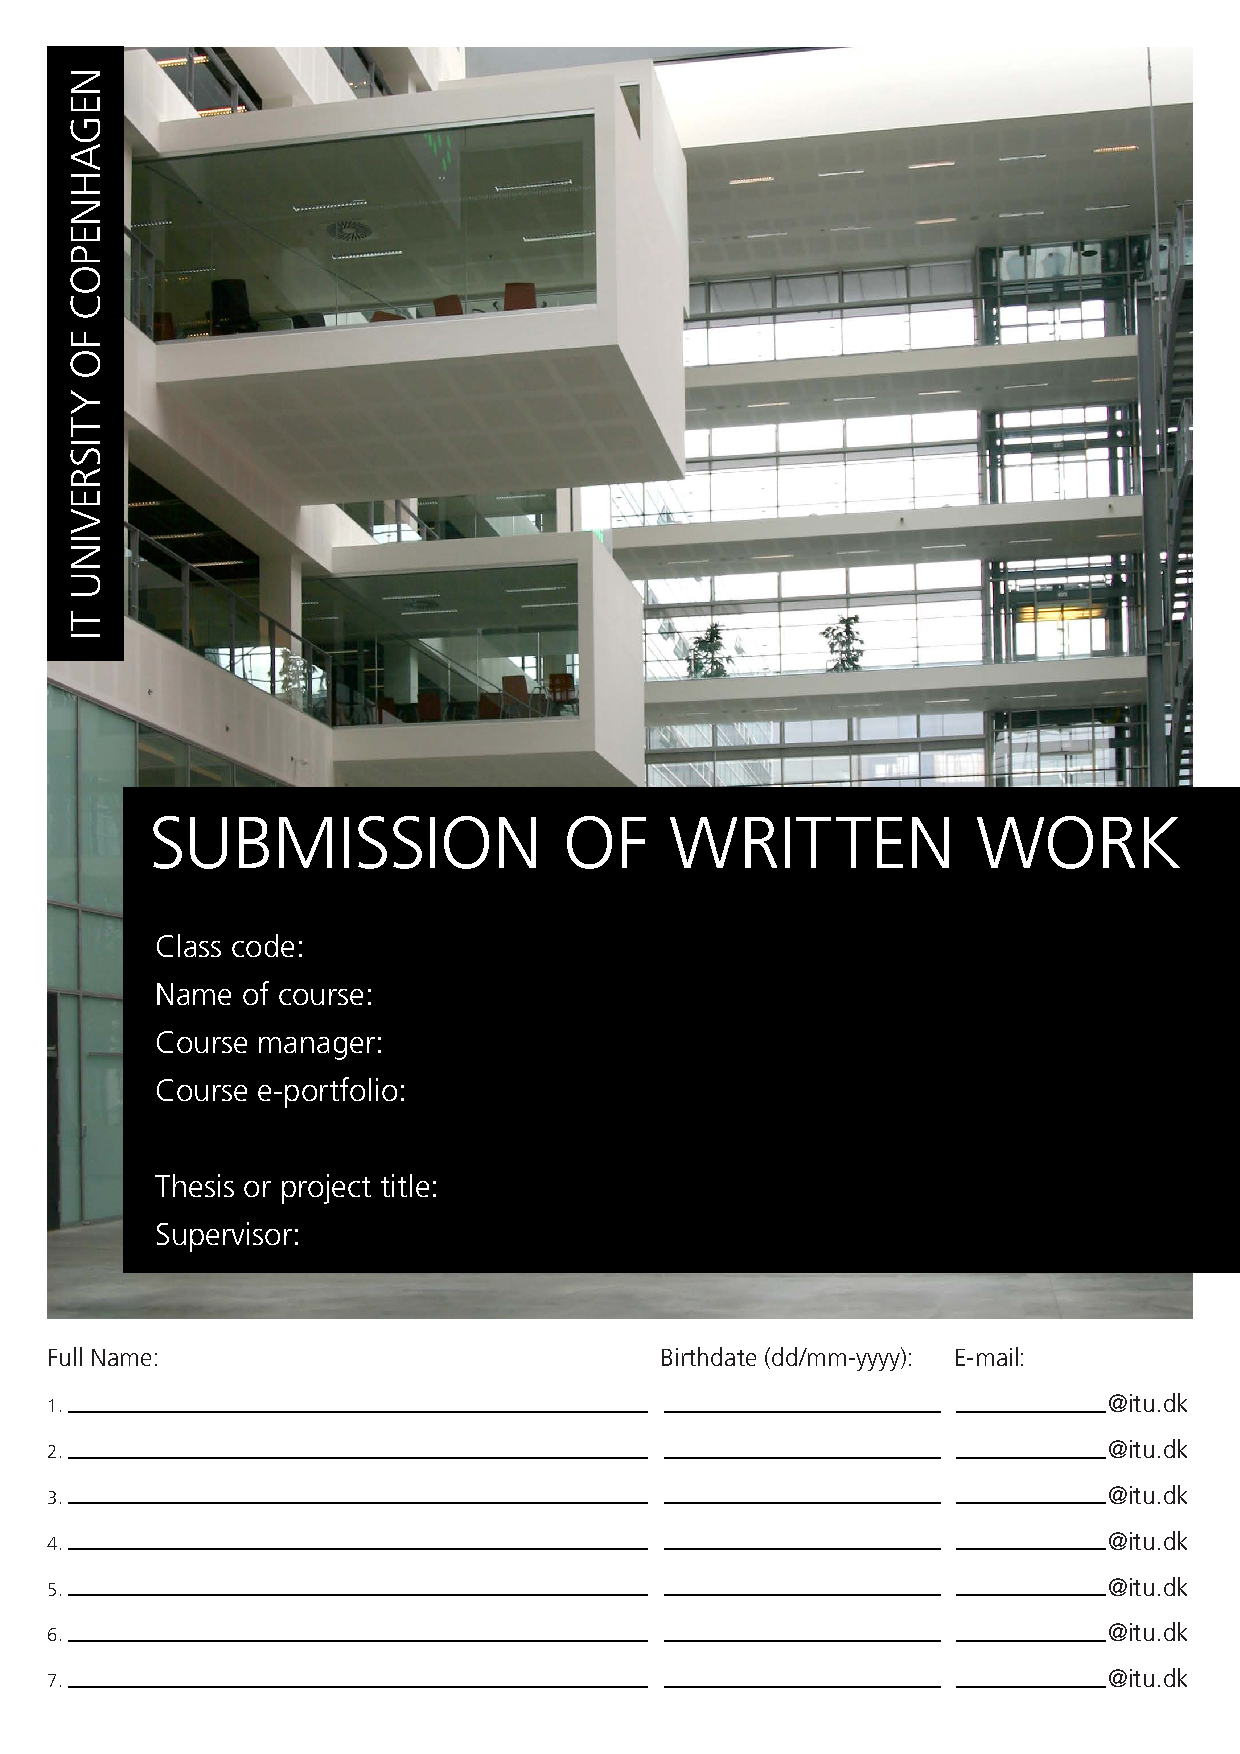
\includepdf[pages=-]{annexes/front-page.pdf}


% -----------------------------------------------------------------------------
% Appendices
% -----------------------------------------------------------------------------
\appendix

% Appendix A: Source Code.
%
% MIT License
%
% Copyright (c) 2024 Fabricio Batista Narcizo.
%
% Permission is hereby granted, free of charge, to any person obtaining a copy
% of this software and associated documentation files (the "Software"), to deal
% in the Software without restriction, including without limitation the rights
% to use, copy, modify, merge, publish, distribute, sublicense, and/or sell
% copies of the Software, and to permit persons to whom the Software is
% furnished to do so, subject to the following conditions:
%
% The above copyright notice and this permission notice shall be included in
% all copies or substantial portions of the Software.
%
% THE SOFTWARE IS PROVIDED "AS IS", WITHOUT WARRANTY OF ANY KIND, EXPRESS OR
% IMPLIED, INCLUDING BUT NOT LIMITED TO THE WARRANTIES OF MERCHANTABILITY,
% FITNESS FOR A PARTICULAR PURPOSE AND NONINFRINGEMENT. IN NO EVENT SHALL THE
% AUTHORS OR COPYRIGHT HOLDERS BE LIABLE FOR ANY CLAIM, DAMAGES OR OTHER
% LIABILITY, WHETHER IN AN ACTION OF CONTRACT, TORT OR OTHERWISE, ARISING FROM,
% OUT OF OR IN CONNECTION WITH THE SOFTWARE OR THE USE OR OTHER DEALINGS IN THE
% SOFTWARE.
%

% Source Code Appendix.
\chapter{Source Code}\label{app:source-code}
\lettrine[lines=3]{P}{lease,} avoid to add source-codes directly in your thesis chapters. Instead, add them as an appendix or in a separate document. This approach ensures that the document remains clean and easy to read. Below is an example of how to include a Python script in the document. See Listing~\ref{lst:cnn_2} for the source code.
\lstinputlisting[
    language=Python,
    belowcaptionskip=15pt,
    label={lst:cnn_2},
    caption={Convolutional neural network implemented in Python using TensorFlow and Keras.}]{codes/cnn_model.py}



% -----------------------------------------------------------------------------
% End of the Document
% -----------------------------------------------------------------------------
\end{document}
